\documentclass[twoside]{book}

% Packages required by doxygen
\usepackage{calc}
\usepackage{doxygen}
\usepackage{graphicx}
\usepackage[utf8]{inputenc}
\usepackage{makeidx}
\usepackage{multicol}
\usepackage{multirow}
\usepackage{textcomp}
\usepackage[table]{xcolor}

% Font selection
\usepackage[T1]{fontenc}
\usepackage{mathptmx}
\usepackage[scaled=.90]{helvet}
\usepackage{courier}
\usepackage{amssymb}
\usepackage{sectsty}
\renewcommand{\familydefault}{\sfdefault}
\allsectionsfont{%
  \fontseries{bc}\selectfont%
  \color{darkgray}%
}
\renewcommand{\DoxyLabelFont}{%
  \fontseries{bc}\selectfont%
  \color{darkgray}%
}

% Page & text layout
\usepackage{geometry}
\geometry{%
  a4paper,%
  top=2.5cm,%
  bottom=2.5cm,%
  left=2.5cm,%
  right=2.5cm%
}
\tolerance=750
\hfuzz=15pt
\hbadness=750
\setlength{\emergencystretch}{15pt}
\setlength{\parindent}{0cm}
\setlength{\parskip}{0.2cm}
\makeatletter
\renewcommand{\paragraph}{%
  \@startsection{paragraph}{4}{0ex}{-1.0ex}{1.0ex}{%
    \normalfont\normalsize\bfseries\SS@parafont%
  }%
}
\renewcommand{\subparagraph}{%
  \@startsection{subparagraph}{5}{0ex}{-1.0ex}{1.0ex}{%
    \normalfont\normalsize\bfseries\SS@subparafont%
  }%
}
\makeatother

% Headers & footers
\usepackage{fancyhdr}
\pagestyle{fancyplain}
\fancyhead[LE]{\fancyplain{}{\bfseries\thepage}}
\fancyhead[CE]{\fancyplain{}{}}
\fancyhead[RE]{\fancyplain{}{\bfseries\leftmark}}
\fancyhead[LO]{\fancyplain{}{\bfseries\rightmark}}
\fancyhead[CO]{\fancyplain{}{}}
\fancyhead[RO]{\fancyplain{}{\bfseries\thepage}}
\fancyfoot[LE]{\fancyplain{}{}}
\fancyfoot[CE]{\fancyplain{}{}}
\fancyfoot[RE]{\fancyplain{}{\bfseries\scriptsize Generated on Thu Apr 9 2015 14\-:18\-:27 for D\-S\-Epp by Doxygen }}
\fancyfoot[LO]{\fancyplain{}{\bfseries\scriptsize Generated on Thu Apr 9 2015 14\-:18\-:27 for D\-S\-Epp by Doxygen }}
\fancyfoot[CO]{\fancyplain{}{}}
\fancyfoot[RO]{\fancyplain{}{}}
\renewcommand{\footrulewidth}{0.4pt}
\renewcommand{\chaptermark}[1]{%
  \markboth{#1}{}%
}
\renewcommand{\sectionmark}[1]{%
  \markright{\thesection\ #1}%
}

% Indices & bibliography
\usepackage{natbib}
\usepackage[titles]{tocloft}
\setcounter{tocdepth}{3}
\setcounter{secnumdepth}{5}
\makeindex

% Hyperlinks (required, but should be loaded last)
\usepackage{ifpdf}
\ifpdf
  \usepackage[pdftex,pagebackref=true]{hyperref}
\else
  \usepackage[ps2pdf,pagebackref=true]{hyperref}
\fi
\hypersetup{%
  colorlinks=true,%
  linkcolor=blue,%
  citecolor=blue,%
  unicode%
}

% Custom commands
\newcommand{\clearemptydoublepage}{%
  \newpage{\pagestyle{empty}\cleardoublepage}%
}


%===== C O N T E N T S =====

\begin{document}

% Titlepage & ToC
\hypersetup{pageanchor=false}
\pagenumbering{roman}
\begin{titlepage}
\vspace*{7cm}
\begin{center}%
{\Large D\-S\-Epp }\\
\vspace*{1cm}
{\large Generated by Doxygen 1.8.6}\\
\vspace*{0.5cm}
{\small Thu Apr 9 2015 14:18:27}\\
\end{center}
\end{titlepage}
\clearemptydoublepage
\tableofcontents
\clearemptydoublepage
\pagenumbering{arabic}
\hypersetup{pageanchor=true}

%--- Begin generated contents ---
\chapter{Hierarchical Index}
\section{Class Hierarchy}
This inheritance list is sorted roughly, but not completely, alphabetically\-:\begin{DoxyCompactList}
\item \contentsline{section}{C\-\_\-\-Abs\-Diagram}{\pageref{class_c___abs_diagram}}{}
\begin{DoxyCompactList}
\item \contentsline{section}{B\-S\-E\-:\-:C\-\_\-\-B\-S\-E}{\pageref{class_b_s_e_1_1_c___b_s_e}}{}
\begin{DoxyCompactList}
\item \contentsline{section}{B\-S\-E\-:\-:C\-\_\-\-B\-S\-E\-\_\-\-Two\-Body}{\pageref{class_b_s_e_1_1_c___b_s_e___two_body}}{}
\begin{DoxyCompactList}
\item \contentsline{section}{B\-S\-E\-:\-:C\-\_\-\-B\-S\-E\-\_\-\-Matrix}{\pageref{class_b_s_e_1_1_c___b_s_e___matrix}}{}
\begin{DoxyCompactList}
\item \contentsline{section}{B\-S\-E\-:\-:C\-\_\-\-B\-S\-E\-\_\-\-Pseudo\-Scalar}{\pageref{class_b_s_e_1_1_c___b_s_e___pseudo_scalar}}{}
\item \contentsline{section}{B\-S\-E\-:\-:C\-\_\-\-B\-S\-E\-\_\-\-Scalar}{\pageref{class_b_s_e_1_1_c___b_s_e___scalar}}{}
\item \contentsline{section}{B\-S\-E\-:\-:C\-\_\-\-B\-S\-E\-\_\-\-Vector}{\pageref{class_b_s_e_1_1_c___b_s_e___vector}}{}
\end{DoxyCompactList}
\end{DoxyCompactList}
\end{DoxyCompactList}
\item \contentsline{section}{Kernels\-:\-:C\-\_\-\-Abstract\-Kernel}{\pageref{class_kernels_1_1_c___abstract_kernel}}{}
\begin{DoxyCompactList}
\item \contentsline{section}{Kernels\-:\-:C\-\_\-\-Two\-Quark\-Kernel}{\pageref{class_kernels_1_1_c___two_quark_kernel}}{}
\begin{DoxyCompactList}
\item \contentsline{section}{Kernels\-:\-:C\-\_\-\-Kernel\-\_\-\-R\-L}{\pageref{class_kernels_1_1_c___kernel___r_l}}{}
\item \contentsline{section}{Kernels\-:\-:C\-\_\-\-Kernel\-\_\-\-R\-L\-\_\-\-P\-S}{\pageref{class_kernels_1_1_c___kernel___r_l___p_s}}{}
\end{DoxyCompactList}
\end{DoxyCompactList}
\item \contentsline{section}{Propagators\-:\-:C\-\_\-\-Propagator}{\pageref{class_propagators_1_1_c___propagator}}{}
\begin{DoxyCompactList}
\item \contentsline{section}{Propagators\-:\-:C\-\_\-\-Gluon}{\pageref{class_propagators_1_1_c___gluon}}{}
\item \contentsline{section}{Propagators\-:\-:C\-\_\-\-Quark}{\pageref{class_propagators_1_1_c___quark}}{}
\begin{DoxyCompactList}
\item \contentsline{section}{Propagators\-:\-:C\-\_\-\-Bottom\-\_\-\-Quark}{\pageref{class_propagators_1_1_c___bottom___quark}}{}
\item \contentsline{section}{Propagators\-:\-:C\-\_\-\-Charm\-\_\-\-Quark}{\pageref{class_propagators_1_1_c___charm___quark}}{}
\item \contentsline{section}{Propagators\-:\-:C\-\_\-\-Down\-\_\-\-Quark}{\pageref{class_propagators_1_1_c___down___quark}}{}
\item \contentsline{section}{Propagators\-:\-:C\-\_\-\-Strange\-\_\-\-Quark}{\pageref{class_propagators_1_1_c___strange___quark}}{}
\item \contentsline{section}{Propagators\-:\-:C\-\_\-\-Test\-\_\-\-Quark}{\pageref{class_propagators_1_1_c___test___quark}}{}
\item \contentsline{section}{Propagators\-:\-:C\-\_\-\-Up\-\_\-\-Quark}{\pageref{class_propagators_1_1_c___up___quark}}{}
\end{DoxyCompactList}
\end{DoxyCompactList}
\end{DoxyCompactList}
\item \contentsline{section}{C\-\_\-\-Abstract\-Builder}{\pageref{class_c___abstract_builder}}{}
\begin{DoxyCompactList}
\item \contentsline{section}{C\-\_\-\-Meson\-Builder}{\pageref{class_c___meson_builder}}{}
\end{DoxyCompactList}
\item \contentsline{section}{Interpolation\-:\-:C\-\_\-\-Base\-\_\-interp}{\pageref{class_interpolation_1_1_c___base__interp}}{}
\begin{DoxyCompactList}
\item \contentsline{section}{Interpolation\-:\-:C\-\_\-\-Bary\-Rat\-\_\-interp}{\pageref{class_interpolation_1_1_c___bary_rat__interp}}{}
\end{DoxyCompactList}
\item \contentsline{section}{C\-\_\-\-Binder}{\pageref{class_c___binder}}{}
\item \contentsline{section}{B\-S\-E\-:\-:C\-\_\-\-Bound\-State\-\_\-parameters}{\pageref{class_b_s_e_1_1_c___bound_state__parameters}}{}
\item \contentsline{section}{B\-S\-E\-:\-:C\-\_\-\-B\-S\-E\-\_\-\-Factory}{\pageref{class_b_s_e_1_1_c___b_s_e___factory}}{}
\item \contentsline{section}{C\-\_\-\-Dedic\-Mem\-\_\-\-Abs}{\pageref{class_c___dedic_mem___abs}}{}
\begin{DoxyCompactList}
\item \contentsline{section}{C\-\_\-\-Dedic\-Mem\-\_\-\-B\-S\-E}{\pageref{class_c___dedic_mem___b_s_e}}{}
\item \contentsline{section}{C\-\_\-\-Dedic\-Mem\-\_\-\-Kernel}{\pageref{class_c___dedic_mem___kernel}}{}
\item \contentsline{section}{C\-\_\-\-Dedic\-Mem\-\_\-\-Quark}{\pageref{class_c___dedic_mem___quark}}{}
\end{DoxyCompactList}
\item \contentsline{section}{Propagators\-:\-:C\-\_\-\-Gluon\-\_\-\-Factory}{\pageref{class_propagators_1_1_c___gluon___factory}}{}
\item \contentsline{section}{C\-\_\-\-Gradiend\-\_\-\-Descent}{\pageref{class_c___gradiend___descent}}{}
\item \contentsline{section}{Integration\-:\-:C\-\_\-\-Integration\-Nodes}{\pageref{class_integration_1_1_c___integration_nodes}}{}
\begin{DoxyCompactList}
\item \contentsline{section}{Integration\-:\-:C\-\_\-\-Integrator\-\_\-\-Line$<$ t\-\_\-cmplx\-Matrix, double $>$}{\pageref{class_integration_1_1_c___integrator___line}}{}
\item \contentsline{section}{Integration\-:\-:C\-\_\-\-Integrator\-\_\-\-Line$<$ T\-\_\-out, T\-\_\-in $>$}{\pageref{class_integration_1_1_c___integrator___line}}{}
\end{DoxyCompactList}
\item \contentsline{section}{Integration\-:\-:C\-\_\-\-Integrator\-\_\-\-Path$<$ T\-\_\-out, T\-\_\-contour, T\-\_\-in $>$}{\pageref{class_integration_1_1_c___integrator___path}}{}
\item \contentsline{section}{Integration\-:\-:C\-\_\-\-Integrator\-\_\-\-Path$<$ t\-\_\-cmplx, t\-\_\-cmplx\-Array2\-D, t\-\_\-cmplx $>$}{\pageref{class_integration_1_1_c___integrator___path}}{}
\item \contentsline{section}{Kernels\-:\-:C\-\_\-\-Kernel\-\_\-\-Factory}{\pageref{class_kernels_1_1_c___kernel___factory}}{}
\item \contentsline{section}{C\-\_\-\-Kinematics\-\_\-1loop}{\pageref{class_c___kinematics__1loop}}{}
\item \contentsline{section}{Interpolation\-:\-:C\-\_\-\-Linear$<$ x\-\_\-type, y\-\_\-type $>$}{\pageref{class_interpolation_1_1_c___linear}}{}
\item \contentsline{section}{Interpolation\-:\-:C\-\_\-\-Linear$<$ t\-\_\-cmplx, t\-\_\-cmplx $>$}{\pageref{class_interpolation_1_1_c___linear}}{}
\item \contentsline{section}{C\-\_\-\-Memory\-Factory\-\_\-\-B\-S\-E}{\pageref{class_c___memory_factory___b_s_e}}{}
\item \contentsline{section}{C\-\_\-\-Memory\-Factory\-\_\-\-Kernel}{\pageref{class_c___memory_factory___kernel}}{}
\item \contentsline{section}{C\-\_\-\-Memory\-Factory\-\_\-\-Quark}{\pageref{class_c___memory_factory___quark}}{}
\item \contentsline{section}{Integration\-:\-:C\-\_\-\-One\-Loop\-Integrator$<$ T\-\_\-out, T\-\_\-in, T\-\_\-arg $>$}{\pageref{class_integration_1_1_c___one_loop_integrator}}{}
\item \contentsline{section}{Integration\-:\-:C\-\_\-\-One\-Loop\-Integrator$<$ t\-\_\-cmplx\-Matrix, double, t\-\_\-cmplx\-Array1\-D $>$}{\pageref{class_integration_1_1_c___one_loop_integrator}}{}
\begin{DoxyCompactList}
\item \contentsline{section}{B\-S\-E\-:\-:C\-\_\-\-B\-S\-E\-\_\-\-Two\-Body}{\pageref{class_b_s_e_1_1_c___b_s_e___two_body}}{}
\item \contentsline{section}{Propagators\-:\-:C\-\_\-\-Quark}{\pageref{class_propagators_1_1_c___quark}}{}
\end{DoxyCompactList}
\item \contentsline{section}{Geometry\-:\-:C\-\_\-\-Parabola\-Contour}{\pageref{class_geometry_1_1_c___parabola_contour}}{}
\item \contentsline{section}{Geometry\-:\-:C\-\_\-\-Path}{\pageref{class_geometry_1_1_c___path}}{}
\begin{DoxyCompactList}
\item \contentsline{section}{Geometry\-:\-:C\-\_\-\-Line}{\pageref{class_geometry_1_1_c___line}}{}
\item \contentsline{section}{Geometry\-:\-:C\-\_\-\-Parabola}{\pageref{class_geometry_1_1_c___parabola}}{}
\end{DoxyCompactList}
\item \contentsline{section}{Propagators\-:\-:C\-\_\-\-Quark\-\_\-\-Factory}{\pageref{class_propagators_1_1_c___quark___factory}}{}
\item \contentsline{section}{Propagators\-:\-:C\-\_\-\-Quark\-\_\-parameters}{\pageref{class_propagators_1_1_c___quark__parameters}}{}
\item \contentsline{section}{C\-\_\-\-Spectra}{\pageref{class_c___spectra}}{}
\end{DoxyCompactList}

\chapter{Class Index}
\section{Class List}
Here are the classes, structs, unions and interfaces with brief descriptions\-:\begin{DoxyCompactList}
\item\contentsline{section}{\hyperlink{class_c___abs_diagram}{C\-\_\-\-Abs\-Diagram} }{\pageref{class_c___abs_diagram}}{}
\item\contentsline{section}{\hyperlink{class_c___abstract_kernel}{C\-\_\-\-Abstract\-Kernel} }{\pageref{class_c___abstract_kernel}}{}
\item\contentsline{section}{\hyperlink{class_c___abs_vertex}{C\-\_\-\-Abs\-Vertex} }{\pageref{class_c___abs_vertex}}{}
\item\contentsline{section}{\hyperlink{class_c___bottom___quark}{C\-\_\-\-Bottom\-\_\-\-Quark} }{\pageref{class_c___bottom___quark}}{}
\item\contentsline{section}{\hyperlink{class_c___b_s_e___abstract___builder}{C\-\_\-\-B\-S\-E\-\_\-\-Abstract\-\_\-\-Builder} }{\pageref{class_c___b_s_e___abstract___builder}}{}
\item\contentsline{section}{\hyperlink{class_c___b_s_e___base}{C\-\_\-\-B\-S\-E\-\_\-\-Base} }{\pageref{class_c___b_s_e___base}}{}
\item\contentsline{section}{\hyperlink{class_c___b_s_e___binder}{C\-\_\-\-B\-S\-E\-\_\-\-Binder} }{\pageref{class_c___b_s_e___binder}}{}
\item\contentsline{section}{\hyperlink{class_c___b_s_e___hadron___base}{C\-\_\-\-B\-S\-E\-\_\-\-Hadron\-\_\-\-Base} }{\pageref{class_c___b_s_e___hadron___base}}{}
\item\contentsline{section}{\hyperlink{class_c___b_s_e___hadron___meson}{C\-\_\-\-B\-S\-E\-\_\-\-Hadron\-\_\-\-Meson} }{\pageref{class_c___b_s_e___hadron___meson}}{}
\item\contentsline{section}{\hyperlink{class_c___b_s_e___hadron__parameters}{C\-\_\-\-B\-S\-E\-\_\-\-Hadron\-\_\-parameters} }{\pageref{class_c___b_s_e___hadron__parameters}}{}
\item\contentsline{section}{\hyperlink{class_c___charm___quark}{C\-\_\-\-Charm\-\_\-\-Quark} }{\pageref{class_c___charm___quark}}{}
\item\contentsline{section}{\hyperlink{class_c___dedic_mem___abs}{C\-\_\-\-Dedic\-Mem\-\_\-\-Abs} }{\pageref{class_c___dedic_mem___abs}}{}
\item\contentsline{section}{\hyperlink{class_c___dedic_mem___b_s_e}{C\-\_\-\-Dedic\-Mem\-\_\-\-B\-S\-E} }{\pageref{class_c___dedic_mem___b_s_e}}{}
\item\contentsline{section}{\hyperlink{class_c___dedic_mem___kernel}{C\-\_\-\-Dedic\-Mem\-\_\-\-Kernel} }{\pageref{class_c___dedic_mem___kernel}}{}
\item\contentsline{section}{\hyperlink{class_c___dedic_mem___quark}{C\-\_\-\-Dedic\-Mem\-\_\-\-Quark} }{\pageref{class_c___dedic_mem___quark}}{}
\item\contentsline{section}{\hyperlink{class_c___down___quark}{C\-\_\-\-Down\-\_\-\-Quark} }{\pageref{class_c___down___quark}}{}
\item\contentsline{section}{\hyperlink{class_c___gluon}{C\-\_\-\-Gluon} }{\pageref{class_c___gluon}}{}
\item\contentsline{section}{\hyperlink{class_c___gluon___factory}{C\-\_\-\-Gluon\-\_\-\-Factory} }{\pageref{class_c___gluon___factory}}{}
\item\contentsline{section}{\hyperlink{class_c___integration___mockup}{C\-\_\-\-Integration\-\_\-\-Mockup} }{\pageref{class_c___integration___mockup}}{}
\item\contentsline{section}{\hyperlink{class_c___integration_nodes}{C\-\_\-\-Integration\-Nodes} }{\pageref{class_c___integration_nodes}}{}
\item\contentsline{section}{\hyperlink{class_c___integrator___line}{C\-\_\-\-Integrator\-\_\-\-Line$<$ T\-\_\-out, T\-\_\-in $>$} }{\pageref{class_c___integrator___line}}{}
\item\contentsline{section}{\hyperlink{class_c___integrator___path}{C\-\_\-\-Integrator\-\_\-\-Path$<$ T\-\_\-out, T\-\_\-contour, T\-\_\-in $>$} }{\pageref{class_c___integrator___path}}{}
\item\contentsline{section}{\hyperlink{class_c___kernel___factory}{C\-\_\-\-Kernel\-\_\-\-Factory} }{\pageref{class_c___kernel___factory}}{}
\item\contentsline{section}{\hyperlink{class_c___kernel___r_l}{C\-\_\-\-Kernel\-\_\-\-R\-L} }{\pageref{class_c___kernel___r_l}}{}
\item\contentsline{section}{\hyperlink{class_c___kernel___r_l___p_s}{C\-\_\-\-Kernel\-\_\-\-R\-L\-\_\-\-P\-S} }{\pageref{class_c___kernel___r_l___p_s}}{}
\item\contentsline{section}{\hyperlink{class_c___kinematics__1loop}{C\-\_\-\-Kinematics\-\_\-1loop} }{\pageref{class_c___kinematics__1loop}}{}
\item\contentsline{section}{\hyperlink{class_geometry_1_1_c___line}{Geometry\-::\-C\-\_\-\-Line} }{\pageref{class_geometry_1_1_c___line}}{}
\item\contentsline{section}{\hyperlink{class_c___memory_factory}{C\-\_\-\-Memory\-Factory} }{\pageref{class_c___memory_factory}}{}
\item\contentsline{section}{\hyperlink{class_c___memory_factory___b_s_e}{C\-\_\-\-Memory\-Factory\-\_\-\-B\-S\-E} }{\pageref{class_c___memory_factory___b_s_e}}{}
\item\contentsline{section}{\hyperlink{class_c___memory_factory___kernel}{C\-\_\-\-Memory\-Factory\-\_\-\-Kernel} }{\pageref{class_c___memory_factory___kernel}}{}
\item\contentsline{section}{\hyperlink{class_c___memory_factory___quark}{C\-\_\-\-Memory\-Factory\-\_\-\-Quark} }{\pageref{class_c___memory_factory___quark}}{}
\item\contentsline{section}{\hyperlink{class_c___meson}{C\-\_\-\-Meson} }{\pageref{class_c___meson}}{}
\item\contentsline{section}{\hyperlink{class_c___mesons___axial_vector}{C\-\_\-\-Mesons\-\_\-\-Axial\-Vector} }{\pageref{class_c___mesons___axial_vector}}{}
\item\contentsline{section}{\hyperlink{class_c___mesons___pseudo_scalar}{C\-\_\-\-Mesons\-\_\-\-Pseudo\-Scalar} }{\pageref{class_c___mesons___pseudo_scalar}}{}
\item\contentsline{section}{\hyperlink{class_c___mesons___scalar}{C\-\_\-\-Mesons\-\_\-\-Scalar} }{\pageref{class_c___mesons___scalar}}{}
\item\contentsline{section}{\hyperlink{class_c___mesons___tensor}{C\-\_\-\-Mesons\-\_\-\-Tensor} }{\pageref{class_c___mesons___tensor}}{}
\item\contentsline{section}{\hyperlink{class_c___mesons___vector}{C\-\_\-\-Mesons\-\_\-\-Vector} }{\pageref{class_c___mesons___vector}}{}
\item\contentsline{section}{\hyperlink{class_c___one_loop_integrator}{C\-\_\-\-One\-Loop\-Integrator$<$ T\-\_\-out, T\-\_\-in, T\-\_\-arg $>$} }{\pageref{class_c___one_loop_integrator}}{}
\item\contentsline{section}{\hyperlink{class_geometry_1_1_c___parabola}{Geometry\-::\-C\-\_\-\-Parabola} }{\pageref{class_geometry_1_1_c___parabola}}{}
\item\contentsline{section}{\hyperlink{class_geometry_1_1_c___parabola_contour}{Geometry\-::\-C\-\_\-\-Parabola\-Contour} }{\pageref{class_geometry_1_1_c___parabola_contour}}{}
\item\contentsline{section}{\hyperlink{class_geometry_1_1_c___path}{Geometry\-::\-C\-\_\-\-Path} }{\pageref{class_geometry_1_1_c___path}}{}
\item\contentsline{section}{\hyperlink{class_c___physical___state}{C\-\_\-\-Physical\-\_\-\-State} }{\pageref{class_c___physical___state}}{}
\item\contentsline{section}{\hyperlink{class_c___propagator}{C\-\_\-\-Propagator} }{\pageref{class_c___propagator}}{}
\item\contentsline{section}{\hyperlink{class_c___propagator___factory}{C\-\_\-\-Propagator\-\_\-\-Factory} }{\pageref{class_c___propagator___factory}}{}
\item\contentsline{section}{\hyperlink{class_c___quark}{C\-\_\-\-Quark} }{\pageref{class_c___quark}}{}
\item\contentsline{section}{\hyperlink{class_c___quark___factory}{C\-\_\-\-Quark\-\_\-\-Factory} }{\pageref{class_c___quark___factory}}{}
\item\contentsline{section}{\hyperlink{class_c___quark__parameters}{C\-\_\-\-Quark\-\_\-parameters} }{\pageref{class_c___quark__parameters}}{}
\item\contentsline{section}{\hyperlink{class_c___strange___quark}{C\-\_\-\-Strange\-\_\-\-Quark} }{\pageref{class_c___strange___quark}}{}
\item\contentsline{section}{\hyperlink{class_c___test___quark}{C\-\_\-\-Test\-\_\-\-Quark} \\*Specific type for unit testing -\/ all quark parameters are default }{\pageref{class_c___test___quark}}{}
\item\contentsline{section}{\hyperlink{class_c___up___quark}{C\-\_\-\-Up\-\_\-\-Quark} }{\pageref{class_c___up___quark}}{}
\item\contentsline{section}{\hyperlink{class_interpolation_1_1_linear}{Interpolation\-::\-Linear$<$ x\-\_\-type, y\-\_\-type $>$} \\*Linearly interpolates a given set of points }{\pageref{class_interpolation_1_1_linear}}{}
\end{DoxyCompactList}

\chapter{Class Documentation}
\hypertarget{class_c___abs_diagram}{\section{C\-\_\-\-Abs\-Diagram Class Reference}
\label{class_c___abs_diagram}\index{C\-\_\-\-Abs\-Diagram@{C\-\_\-\-Abs\-Diagram}}
}
Inheritance diagram for C\-\_\-\-Abs\-Diagram\-:\begin{figure}[H]
\begin{center}
\leavevmode
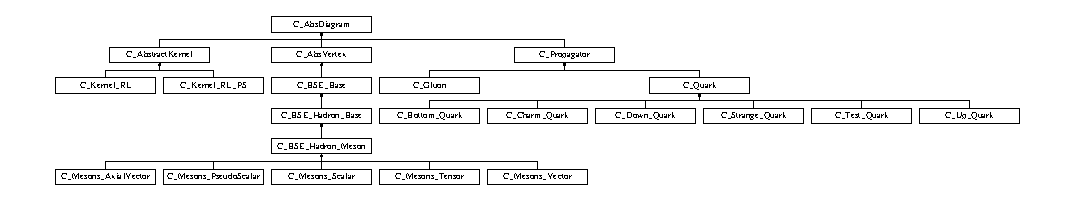
\includegraphics[height=2.248996cm]{class_c___abs_diagram}
\end{center}
\end{figure}
\subsection*{Public Member Functions}
\begin{DoxyCompactItemize}
\item 
\hypertarget{class_c___abs_diagram_a88baf4e9d29753417b7e65ef18f0b28f}{void {\bfseries Set\-Name\-I\-D} (string \-\_\-name, int \-\_\-\-I\-D)}\label{class_c___abs_diagram_a88baf4e9d29753417b7e65ef18f0b28f}

\item 
\hypertarget{class_c___abs_diagram_a5a52da1cfd635da06a6bfdd002e7f674}{void {\bfseries Get\-Name\-I\-D} ()}\label{class_c___abs_diagram_a5a52da1cfd635da06a6bfdd002e7f674}

\end{DoxyCompactItemize}
\subsection*{Protected Attributes}
\begin{DoxyCompactItemize}
\item 
\hypertarget{class_c___abs_diagram_a919d23735a009dc5a78e02e01e1eb40b}{string {\bfseries name}}\label{class_c___abs_diagram_a919d23735a009dc5a78e02e01e1eb40b}

\item 
\hypertarget{class_c___abs_diagram_a08de955405ee0344287b2eb5f6cb62b5}{int {\bfseries I\-D}}\label{class_c___abs_diagram_a08de955405ee0344287b2eb5f6cb62b5}

\item 
\hypertarget{class_c___abs_diagram_a958ffee1be22aa70a0e2eb9fa44f5784}{Dirac\-Gamma \hyperlink{class_c___abs_diagram_a958ffee1be22aa70a0e2eb9fa44f5784}{Z}}\label{class_c___abs_diagram_a958ffee1be22aa70a0e2eb9fa44f5784}

\begin{DoxyCompactList}\small\item\em Dirac gamma matrices $ \gamma_\mu $. \end{DoxyCompactList}\item 
\hypertarget{class_c___abs_diagram_a4eded4aff0f19920d9ec52e2f5c63abf}{Dirac\-Gamma {\bfseries Y}}\label{class_c___abs_diagram_a4eded4aff0f19920d9ec52e2f5c63abf}

\item 
\hypertarget{class_c___abs_diagram_a31794dd2c315f6bf18e2908d669ccc61}{Dirac\-Gamma5 \hyperlink{class_c___abs_diagram_a31794dd2c315f6bf18e2908d669ccc61}{\-\_\-\-Y5}}\label{class_c___abs_diagram_a31794dd2c315f6bf18e2908d669ccc61}

\begin{DoxyCompactList}\small\item\em Dirac gamma matrix $ \gamma_5 $. \end{DoxyCompactList}\item 
\hypertarget{class_c___abs_diagram_ac4646ab596ff13dd531f28f755d3dd4e}{Dirac\-Sigma \hyperlink{class_c___abs_diagram_ac4646ab596ff13dd531f28f755d3dd4e}{S\-I\-G}}\label{class_c___abs_diagram_ac4646ab596ff13dd531f28f755d3dd4e}

\begin{DoxyCompactList}\small\item\em Dirac sigma matrix $ \sigma_{\mu\nu} $. \end{DoxyCompactList}\item 
\hypertarget{class_c___abs_diagram_a4daaf1d6cbcb0aa0bc93417eb11b49a4}{Metric\-Tensor \hyperlink{class_c___abs_diagram_a4daaf1d6cbcb0aa0bc93417eb11b49a4}{g}}\label{class_c___abs_diagram_a4daaf1d6cbcb0aa0bc93417eb11b49a4}

\begin{DoxyCompactList}\small\item\em Euclidean metric tensor $ g_{\mu\nu} $. \end{DoxyCompactList}\item 
\hypertarget{class_c___abs_diagram_aff57681049aaff10af1fd2a0151209b8}{t\-\_\-cmplx\-Dirac \hyperlink{class_c___abs_diagram_aff57681049aaff10af1fd2a0151209b8}{I}}\label{class_c___abs_diagram_aff57681049aaff10af1fd2a0151209b8}

\begin{DoxyCompactList}\small\item\em Unit matrix (4,4) in Dirac space. \end{DoxyCompactList}\item 
\hypertarget{class_c___abs_diagram_a49ab5b499fd64c4a196349730d4beda3}{t\-\_\-cmplx\-Dirac {\bfseries Y5}}\label{class_c___abs_diagram_a49ab5b499fd64c4a196349730d4beda3}

\item 
\hypertarget{class_c___abs_diagram_a3e24081668fb3198fd043dd291fba4c5}{double {\bfseries pi}}\label{class_c___abs_diagram_a3e24081668fb3198fd043dd291fba4c5}

\item 
\hypertarget{class_c___abs_diagram_aa3cfb09af9c9e81fa1af3a78b5d667a7}{t\-\_\-cmplx \hyperlink{class_c___abs_diagram_aa3cfb09af9c9e81fa1af3a78b5d667a7}{ii}}\label{class_c___abs_diagram_aa3cfb09af9c9e81fa1af3a78b5d667a7}

\begin{DoxyCompactList}\small\item\em Imaginary unit. \end{DoxyCompactList}\end{DoxyCompactItemize}


The documentation for this class was generated from the following file\-:\begin{DoxyCompactItemize}
\item 
source/\-Abs/Abs\-Diagram.\-hpp\end{DoxyCompactItemize}

\hypertarget{class_c___abstract_kernel}{\section{C\-\_\-\-Abstract\-Kernel Class Reference}
\label{class_c___abstract_kernel}\index{C\-\_\-\-Abstract\-Kernel@{C\-\_\-\-Abstract\-Kernel}}
}
Inheritance diagram for C\-\_\-\-Abstract\-Kernel\-:\begin{figure}[H]
\begin{center}
\leavevmode
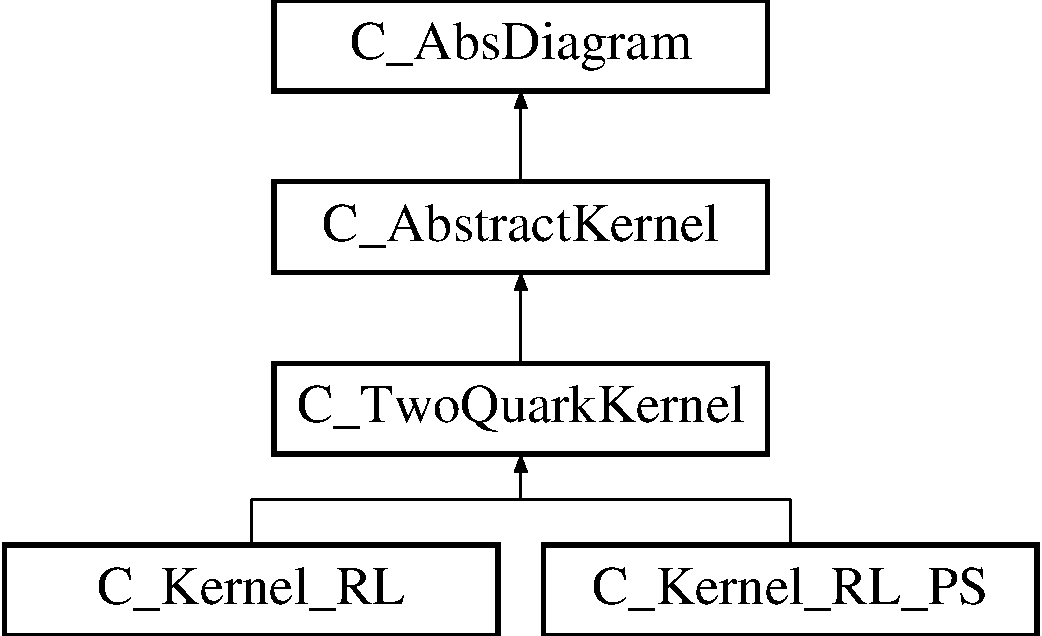
\includegraphics[height=3.000000cm]{class_c___abstract_kernel}
\end{center}
\end{figure}
\subsection*{Public Member Functions}
\begin{DoxyCompactItemize}
\item 
\hypertarget{class_c___abstract_kernel_a6a6510a5e44b78d22c6b1287121074c7}{virtual void {\bfseries info} ()=0}\label{class_c___abstract_kernel_a6a6510a5e44b78d22c6b1287121074c7}

\item 
\hypertarget{class_c___abstract_kernel_af2656096f4bb6b293b7c6fd6b98e1852}{void {\bfseries set\-Exchange\-I\-D} (P\-S\-\_\-type\-\_\-\-I\-D exchange\-\_\-id)}\label{class_c___abstract_kernel_af2656096f4bb6b293b7c6fd6b98e1852}

\item 
\hypertarget{class_c___abstract_kernel_a732c7cfecc0f30cd585734b4a3b2f5d0}{Kernel\-\_\-\-I\-D {\bfseries Kernel\-I\-D} ()}\label{class_c___abstract_kernel_a732c7cfecc0f30cd585734b4a3b2f5d0}

\item 
\hypertarget{class_c___abstract_kernel_a7f4d733129fb96fc6b3964c6b2ef696d}{void {\bfseries set\-Propagators} (std\-::vector$<$ \hyperlink{class_c___propagator}{C\-\_\-\-Propagator} $\ast$ $>$ \-\_\-\-\_\-\-Propagators)}\label{class_c___abstract_kernel_a7f4d733129fb96fc6b3964c6b2ef696d}

\item 
\hypertarget{class_c___abstract_kernel_a44d9413f79dcb3581f6f626dcaabda94}{virtual void {\bfseries set\-Convolution\-Type} (int type)}\label{class_c___abstract_kernel_a44d9413f79dcb3581f6f626dcaabda94}

\item 
\hypertarget{class_c___abstract_kernel_a0589cd3db4acff68cb08f7150bc3c994}{t\-\_\-cmplx {\bfseries Trace\-Kernel\-Without\-Storing} (t\-\_\-cmplx\-Dirac \&Projector, t\-\_\-cmplx\-Dirac \&Wave\-Func, t\-\_\-cmplx\-Vector \&k, t\-\_\-cmplx\-Vector \&p, t\-\_\-cmplx\-Vector \&P, bool flag\-\_\-reset\-\_\-kernel)}\label{class_c___abstract_kernel_a0589cd3db4acff68cb08f7150bc3c994}

\item 
\hypertarget{class_c___abstract_kernel_af7b68da40937efab335f2f3dc85a0aac}{void {\bfseries set\-K\-Matrix\-Thread\-Storage} (t\-\_\-cmplx\-Vector \&k, t\-\_\-cmplx\-Vector \&p, t\-\_\-cmplx\-Vector \&P)}\label{class_c___abstract_kernel_af7b68da40937efab335f2f3dc85a0aac}

\item 
\hypertarget{class_c___abstract_kernel_a1bc1d99206e76ab535e2b22c65587b66}{t\-\_\-cmplx {\bfseries take\-Inner\-Product} (t\-\_\-cmplx\-Tensor \&A, t\-\_\-cmplx\-Tensor \&B, int rank)}\label{class_c___abstract_kernel_a1bc1d99206e76ab535e2b22c65587b66}

\item 
\hypertarget{class_c___abstract_kernel_a2f2a68781d4bcd8cb7e12f6ae149f22f}{void {\bfseries resize\-Kmatrix} (t\-\_\-cmplx\-Matrix2\-D \&K\-\_\-matrix)}\label{class_c___abstract_kernel_a2f2a68781d4bcd8cb7e12f6ae149f22f}

\item 
\hypertarget{class_c___abstract_kernel_a93c0cd44a8327c5afa956f39713bc94a}{virtual void {\bfseries set\-Mediators} (t\-\_\-cmplx\-Vector \&k, t\-\_\-cmplx\-Vector \&p, t\-\_\-cmplx\-Vector \&P, std\-::vector$<$ t\-\_\-cmplx\-Tensor $>$ \&Mediators)=0}\label{class_c___abstract_kernel_a93c0cd44a8327c5afa956f39713bc94a}

\item 
\hypertarget{class_c___abstract_kernel_ad90e029ee7da0a8aee835a0e12ee569f}{virtual t\-\_\-cmplx {\bfseries Element\-Kmatrix} (int t, int s, int r, int u, std\-::vector$<$ t\-\_\-cmplx\-Tensor $>$ \&Mediators)=0}\label{class_c___abstract_kernel_ad90e029ee7da0a8aee835a0e12ee569f}

\item 
\hypertarget{class_c___abstract_kernel_a8a46c6a478ff8c4cef966a011ddf4cc3}{void {\bfseries set\-Kmatrix} (t\-\_\-cmplx\-Matrix2\-D \&K\-\_\-matrix, std\-::vector$<$ t\-\_\-cmplx\-Tensor $>$ \&Mediators)}\label{class_c___abstract_kernel_a8a46c6a478ff8c4cef966a011ddf4cc3}

\end{DoxyCompactItemize}
\subsection*{Static Public Member Functions}
\begin{DoxyCompactItemize}
\item 
\hypertarget{class_c___abstract_kernel_a8e4523d9df8882a20b01e511d05815f0}{static \hyperlink{class_c___abstract_kernel}{C\-\_\-\-Abstract\-Kernel} $\ast$ {\bfseries create\-Kernel} (Kernel\-\_\-\-I\-D id)}\label{class_c___abstract_kernel_a8e4523d9df8882a20b01e511d05815f0}

\end{DoxyCompactItemize}
\subsection*{Public Attributes}
\begin{DoxyCompactItemize}
\item 
\hypertarget{class_c___abstract_kernel_a490aac141740e9ee3c4d2b0c0dcb77c7}{\hyperlink{class_c___dedic_mem___kernel}{C\-\_\-\-Dedic\-Mem\-\_\-\-Kernel} $\ast$ {\bfseries Memory}}\label{class_c___abstract_kernel_a490aac141740e9ee3c4d2b0c0dcb77c7}

\end{DoxyCompactItemize}
\subsection*{Protected Attributes}
\begin{DoxyCompactItemize}
\item 
\hypertarget{class_c___abstract_kernel_aa60e6339b256ab24d835f35520df5052}{std\-::vector$<$ \hyperlink{class_c___propagator}{C\-\_\-\-Propagator} $\ast$ $>$ \hyperlink{class_c___abstract_kernel_aa60e6339b256ab24d835f35520df5052}{Propagators}}\label{class_c___abstract_kernel_aa60e6339b256ab24d835f35520df5052}

\begin{DoxyCompactList}\small\item\em vector of pointer to prapagator as two-\/body scattering mediators \end{DoxyCompactList}\item 
\hypertarget{class_c___abstract_kernel_aac115b60d8e20bd58262b92e403f0750}{std\-::vector$<$ t\-\_\-cmplx\-Matrix2\-D $>$ \hyperlink{class_c___abstract_kernel_aac115b60d8e20bd58262b92e403f0750}{threadloc\-\_\-\-K\-Matrix}}\label{class_c___abstract_kernel_aac115b60d8e20bd58262b92e403f0750}

\begin{DoxyCompactList}\small\item\em T\-O\-D\-O to include vector of general vertexes. \end{DoxyCompactList}\item 
\hypertarget{class_c___abstract_kernel_a2752ba2a46e476d657e8199cf55c2b3c}{Kernel\-\_\-\-I\-D {\bfseries Kernel\-\_\-type\-\_\-\-I\-D}}\label{class_c___abstract_kernel_a2752ba2a46e476d657e8199cf55c2b3c}

\item 
\hypertarget{class_c___abstract_kernel_a20b072a954f3f1ec0cd78350f1871cf8}{P\-S\-\_\-type\-\_\-\-I\-D {\bfseries Exchange\-\_\-type\-\_\-\-I\-D}}\label{class_c___abstract_kernel_a20b072a954f3f1ec0cd78350f1871cf8}

\end{DoxyCompactItemize}


The documentation for this class was generated from the following files\-:\begin{DoxyCompactItemize}
\item 
source/\-Kernel/Abstract\-Kernel.\-hpp\item 
source/\-Kernel/Kernel\-Factory.\-hpp\end{DoxyCompactItemize}

\hypertarget{class_c___abs_vertex}{\section{C\-\_\-\-Abs\-Vertex Class Reference}
\label{class_c___abs_vertex}\index{C\-\_\-\-Abs\-Vertex@{C\-\_\-\-Abs\-Vertex}}
}
Inheritance diagram for C\-\_\-\-Abs\-Vertex\-:\begin{figure}[H]
\begin{center}
\leavevmode
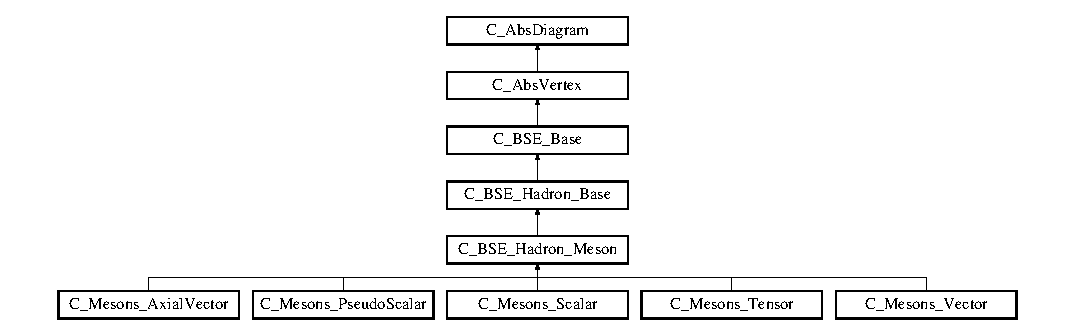
\includegraphics[height=4.048193cm]{class_c___abs_vertex}
\end{center}
\end{figure}
\subsection*{Public Member Functions}
\begin{DoxyCompactItemize}
\item 
\hypertarget{class_c___abs_vertex_a77761b8e56afe2536b821836ca372f63}{void {\bfseries info} ()}\label{class_c___abs_vertex_a77761b8e56afe2536b821836ca372f63}

\item 
\hypertarget{class_c___abs_vertex_af811c4349945a365f9a21caefd331ed3}{virtual void {\bfseries Initialization} ()=0}\label{class_c___abs_vertex_af811c4349945a365f9a21caefd331ed3}

\end{DoxyCompactItemize}
\subsection*{Additional Inherited Members}


The documentation for this class was generated from the following file\-:\begin{DoxyCompactItemize}
\item 
source/\-Vertex/Abs\-Vertex.\-hpp\end{DoxyCompactItemize}

\hypertarget{class_c___bottom___quark}{\section{C\-\_\-\-Bottom\-\_\-\-Quark Class Reference}
\label{class_c___bottom___quark}\index{C\-\_\-\-Bottom\-\_\-\-Quark@{C\-\_\-\-Bottom\-\_\-\-Quark}}
}
Inheritance diagram for C\-\_\-\-Bottom\-\_\-\-Quark\-:\begin{figure}[H]
\begin{center}
\leavevmode
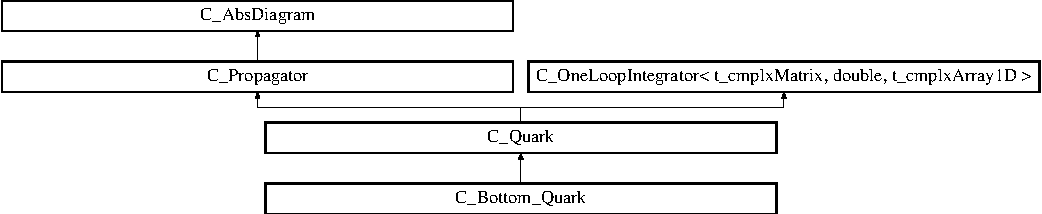
\includegraphics[height=2.871795cm]{class_c___bottom___quark}
\end{center}
\end{figure}
\subsection*{Public Member Functions}
\begin{DoxyCompactItemize}
\item 
\hypertarget{class_c___bottom___quark_a85bf3405a3e4d7e5916a64b996ab621e}{void {\bfseries info} ()}\label{class_c___bottom___quark_a85bf3405a3e4d7e5916a64b996ab621e}

\end{DoxyCompactItemize}
\subsection*{Additional Inherited Members}


The documentation for this class was generated from the following file\-:\begin{DoxyCompactItemize}
\item 
source/\-D\-S\-E/Quark\-Types.\-hpp\end{DoxyCompactItemize}

\hypertarget{class_c___b_s_e___abstract___builder}{\section{C\-\_\-\-B\-S\-E\-\_\-\-Abstract\-\_\-\-Builder Class Reference}
\label{class_c___b_s_e___abstract___builder}\index{C\-\_\-\-B\-S\-E\-\_\-\-Abstract\-\_\-\-Builder@{C\-\_\-\-B\-S\-E\-\_\-\-Abstract\-\_\-\-Builder}}
}
Inheritance diagram for C\-\_\-\-B\-S\-E\-\_\-\-Abstract\-\_\-\-Builder\-:\begin{figure}[H]
\begin{center}
\leavevmode
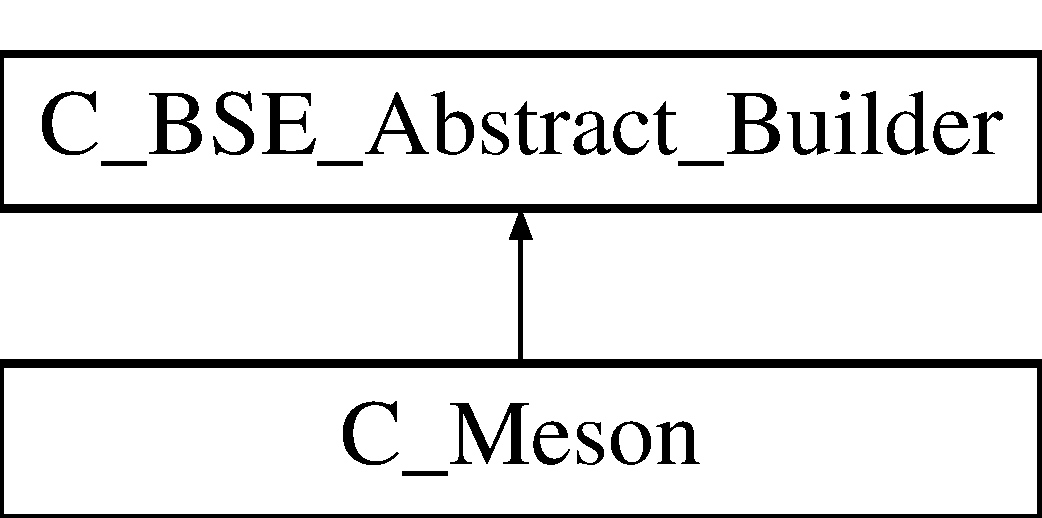
\includegraphics[height=2.000000cm]{class_c___b_s_e___abstract___builder}
\end{center}
\end{figure}
\subsection*{Public Member Functions}
\begin{DoxyCompactItemize}
\item 
\hypertarget{class_c___b_s_e___abstract___builder_a3f7822420d57f9ab4d858462b2b0c025}{\hyperlink{class_c___physical___state}{C\-\_\-\-Physical\-\_\-\-State} $\ast$ {\bfseries Get\-Physical\-State} ()}\label{class_c___b_s_e___abstract___builder_a3f7822420d57f9ab4d858462b2b0c025}

\item 
\hypertarget{class_c___b_s_e___abstract___builder_aaff489dcaf76185835f8cbdc813d587f}{void {\bfseries create\-New\-Physical\-State} ()}\label{class_c___b_s_e___abstract___builder_aaff489dcaf76185835f8cbdc813d587f}

\item 
\hypertarget{class_c___b_s_e___abstract___builder_a313d2a39237b8382af4135c39fe5c333}{virtual void {\bfseries build\-Propagators} ()=0}\label{class_c___b_s_e___abstract___builder_a313d2a39237b8382af4135c39fe5c333}

\item 
\hypertarget{class_c___b_s_e___abstract___builder_a2badc8ce81676b7b4b11f4e1b2abe5b8}{virtual void {\bfseries build\-Kernels} ()=0}\label{class_c___b_s_e___abstract___builder_a2badc8ce81676b7b4b11f4e1b2abe5b8}

\item 
\hypertarget{class_c___b_s_e___abstract___builder_a07dfdd24a8fea467d063a751fc6cae4f}{virtual void {\bfseries build\-B\-S\-Es} ()=0}\label{class_c___b_s_e___abstract___builder_a07dfdd24a8fea467d063a751fc6cae4f}

\item 
\hypertarget{class_c___b_s_e___abstract___builder_a61f6cb37d934ce2b9d68fcb905df63b0}{virtual void {\bfseries Link\-Them\-All} ()=0}\label{class_c___b_s_e___abstract___builder_a61f6cb37d934ce2b9d68fcb905df63b0}

\end{DoxyCompactItemize}
\subsection*{Public Attributes}
\begin{DoxyCompactItemize}
\item 
\hypertarget{class_c___b_s_e___abstract___builder_a95bb89c8179deb6efd51aa5a994f751f}{\hyperlink{class_c___physical___state}{C\-\_\-\-Physical\-\_\-\-State} $\ast$ {\bfseries Physical\-State}}\label{class_c___b_s_e___abstract___builder_a95bb89c8179deb6efd51aa5a994f751f}

\item 
\hypertarget{class_c___b_s_e___abstract___builder_a511633808f27815b4715bb3df2951b2a}{\hyperlink{class_c___quark___factory}{C\-\_\-\-Quark\-\_\-\-Factory} $\ast$ {\bfseries Quark\-Factory}}\label{class_c___b_s_e___abstract___builder_a511633808f27815b4715bb3df2951b2a}

\item 
\hypertarget{class_c___b_s_e___abstract___builder_a5043032a003b92e57ff8dd16e16b4677}{\hyperlink{class_c___gluon___factory}{C\-\_\-\-Gluon\-\_\-\-Factory} $\ast$ {\bfseries Gluon\-Factory}}\label{class_c___b_s_e___abstract___builder_a5043032a003b92e57ff8dd16e16b4677}

\item 
\hypertarget{class_c___b_s_e___abstract___builder_a8c94f78e1427657eac69b287e6599590}{\hyperlink{class_c___kernel___factory}{C\-\_\-\-Kernel\-\_\-\-Factory} $\ast$ {\bfseries Kernel\-Factory}}\label{class_c___b_s_e___abstract___builder_a8c94f78e1427657eac69b287e6599590}

\end{DoxyCompactItemize}


The documentation for this class was generated from the following file\-:\begin{DoxyCompactItemize}
\item 
source/\-Vertex/\-B\-S\-E/B\-S\-E\-\_\-\-Builder.\-hpp\end{DoxyCompactItemize}

\hypertarget{class_c___b_s_e___base}{\section{C\-\_\-\-B\-S\-E\-\_\-\-Base Class Reference}
\label{class_c___b_s_e___base}\index{C\-\_\-\-B\-S\-E\-\_\-\-Base@{C\-\_\-\-B\-S\-E\-\_\-\-Base}}
}
Inheritance diagram for C\-\_\-\-B\-S\-E\-\_\-\-Base\-:\begin{figure}[H]
\begin{center}
\leavevmode
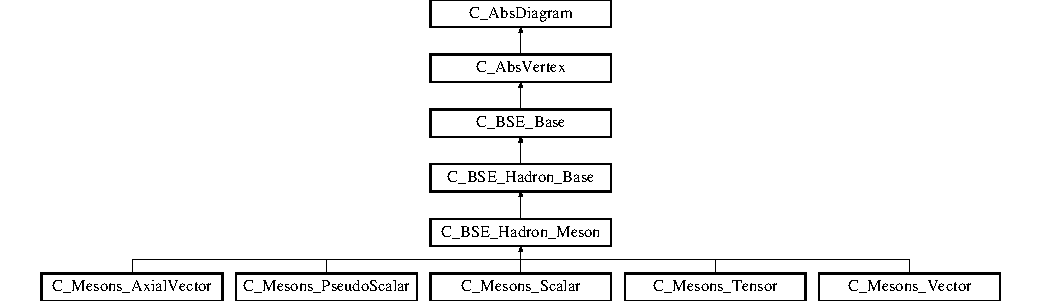
\includegraphics[height=4.048193cm]{class_c___b_s_e___base}
\end{center}
\end{figure}
\subsection*{Public Member Functions}
\begin{DoxyCompactItemize}
\item 
\hypertarget{class_c___b_s_e___base_a4a6278f1af16d8dc05cb59d5c9bea095}{void {\bfseries Link\-To\-Kernel} (\hyperlink{class_c___abstract_kernel}{C\-\_\-\-Abstract\-Kernel} $\ast$\-\_\-\-K)}\label{class_c___b_s_e___base_a4a6278f1af16d8dc05cb59d5c9bea095}

\end{DoxyCompactItemize}
\subsection*{Public Attributes}
\begin{DoxyCompactItemize}
\item 
\hypertarget{class_c___b_s_e___base_ac0079454bdbd7d5064b4cec334abd0ec}{\hyperlink{class_c___dedic_mem___b_s_e}{C\-\_\-\-Dedic\-Mem\-\_\-\-B\-S\-E} $\ast$ {\bfseries Memory}}\label{class_c___b_s_e___base_ac0079454bdbd7d5064b4cec334abd0ec}

\end{DoxyCompactItemize}
\subsection*{Protected Attributes}
\begin{DoxyCompactItemize}
\item 
\hypertarget{class_c___b_s_e___base_a80e4c34e7e5a70051f29392af3f0a4d6}{\hyperlink{class_c___abstract_kernel}{C\-\_\-\-Abstract\-Kernel} $\ast$ {\bfseries Kernel}}\label{class_c___b_s_e___base_a80e4c34e7e5a70051f29392af3f0a4d6}

\item 
\hypertarget{class_c___b_s_e___base_a4d3fd8c389600935b97a4e4131663451}{t\-\_\-cmplx\-Dirac {\bfseries S\-\_\-p}}\label{class_c___b_s_e___base_a4d3fd8c389600935b97a4e4131663451}

\item 
\hypertarget{class_c___b_s_e___base_af6aec03e6379d0da807aba163996dbad}{t\-\_\-cmplx\-Dirac {\bfseries S\-\_\-m}}\label{class_c___b_s_e___base_af6aec03e6379d0da807aba163996dbad}

\item 
\hypertarget{class_c___b_s_e___base_a890241f1da07fd911cae4c81554c654e}{t\-\_\-cmplx\-Dirac {\bfseries Y\-\_\-\-T}}\label{class_c___b_s_e___base_a890241f1da07fd911cae4c81554c654e}

\item 
\hypertarget{class_c___b_s_e___base_a3cf8ecfeabef2d1189002b266da65282}{\hyperlink{class_c___propagator}{C\-\_\-\-Propagator} $\ast$ {\bfseries Parton\-\_\-\-P}}\label{class_c___b_s_e___base_a3cf8ecfeabef2d1189002b266da65282}

\item 
\hypertarget{class_c___b_s_e___base_a0a17d7cfe4c2e33736c2854bd5274a96}{\hyperlink{class_c___propagator}{C\-\_\-\-Propagator} $\ast$ {\bfseries Parton\-\_\-\-M}}\label{class_c___b_s_e___base_a0a17d7cfe4c2e33736c2854bd5274a96}

\end{DoxyCompactItemize}


The documentation for this class was generated from the following file\-:\begin{DoxyCompactItemize}
\item 
source/\-Vertex/\-B\-S\-E/B\-S\-E\-\_\-\-Base.\-hpp\end{DoxyCompactItemize}

\hypertarget{class_c___b_s_e___binder}{\section{C\-\_\-\-B\-S\-E\-\_\-\-Binder Class Reference}
\label{class_c___b_s_e___binder}\index{C\-\_\-\-B\-S\-E\-\_\-\-Binder@{C\-\_\-\-B\-S\-E\-\_\-\-Binder}}
}
\subsection*{Public Member Functions}
\begin{DoxyCompactItemize}
\item 
\hypertarget{class_c___b_s_e___binder_a63c48a6bbd215b094516082a4d58abee}{void {\bfseries Set\-B\-S\-E\-Builder} (\hyperlink{class_c___b_s_e___abstract___builder}{C\-\_\-\-B\-S\-E\-\_\-\-Abstract\-\_\-\-Builder} $\ast$b)}\label{class_c___b_s_e___binder_a63c48a6bbd215b094516082a4d58abee}

\item 
\hypertarget{class_c___b_s_e___binder_adbc4866aa3784e0109321721a9b68d53}{\hyperlink{class_c___physical___state}{C\-\_\-\-Physical\-\_\-\-State} $\ast$ {\bfseries Get\-Physical\-State} ()}\label{class_c___b_s_e___binder_adbc4866aa3784e0109321721a9b68d53}

\item 
\hypertarget{class_c___b_s_e___binder_a098ad5121c3349dfb908653fc82249ef}{void {\bfseries Construct\-Phys\-State} ()}\label{class_c___b_s_e___binder_a098ad5121c3349dfb908653fc82249ef}

\end{DoxyCompactItemize}


The documentation for this class was generated from the following file\-:\begin{DoxyCompactItemize}
\item 
source/\-Vertex/\-B\-S\-E/B\-S\-E\-\_\-\-Builder.\-hpp\end{DoxyCompactItemize}

\hypertarget{class_c___b_s_e___hadron___base}{\section{C\-\_\-\-B\-S\-E\-\_\-\-Hadron\-\_\-\-Base Class Reference}
\label{class_c___b_s_e___hadron___base}\index{C\-\_\-\-B\-S\-E\-\_\-\-Hadron\-\_\-\-Base@{C\-\_\-\-B\-S\-E\-\_\-\-Hadron\-\_\-\-Base}}
}
Inheritance diagram for C\-\_\-\-B\-S\-E\-\_\-\-Hadron\-\_\-\-Base\-:\begin{figure}[H]
\begin{center}
\leavevmode
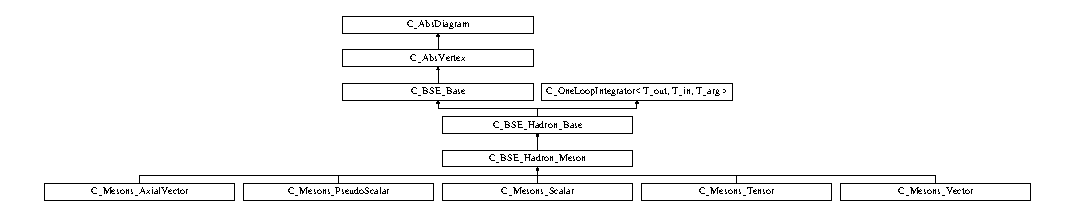
\includegraphics[height=2.470588cm]{class_c___b_s_e___hadron___base}
\end{center}
\end{figure}
\subsection*{Public Member Functions}
\begin{DoxyCompactItemize}
\item 
\hypertarget{class_c___b_s_e___hadron___base_ae90398cf83f468f5c7abda0f73d7b93a}{void {\bfseries set\-Propagators} (t\-\_\-cmplx\-Vector $\ast$K\-\_\-plus, t\-\_\-cmplx\-Vector $\ast$K\-\_\-minus)}\label{class_c___b_s_e___hadron___base_ae90398cf83f468f5c7abda0f73d7b93a}

\item 
\hypertarget{class_c___b_s_e___hadron___base_aa4f6a7802c962d980432254efeb1d432}{virtual void {\bfseries Set\-Dirac\-Structures} (t\-\_\-cmplx\-Vector \-\_\-k, t\-\_\-cmplx\-Vector \-\_\-\-P, std\-::vector$<$ t\-\_\-cmplx\-Dirac $>$ $\ast$Dirac\-Structure)}\label{class_c___b_s_e___hadron___base_aa4f6a7802c962d980432254efeb1d432}

\item 
\hypertarget{class_c___b_s_e___hadron___base_a8d1eac0e1cfc8abd52ef54389eebbf72}{virtual void {\bfseries Set\-Wave\-Functions} ()}\label{class_c___b_s_e___hadron___base_a8d1eac0e1cfc8abd52ef54389eebbf72}

\item 
\hypertarget{class_c___b_s_e___hadron___base_a8cfb0b4fe51a312ad7232bd0fa4c1ccf}{virtual t\-\_\-cmplx\-Matrix {\bfseries Get\-B\-S\-A} ()}\label{class_c___b_s_e___hadron___base_a8cfb0b4fe51a312ad7232bd0fa4c1ccf}

\item 
\hypertarget{class_c___b_s_e___hadron___base_ac42953ea725bd1bd160453e1a11b266f}{virtual t\-\_\-cmplx\-Matrix {\bfseries Get\-B\-S\-A\-\_\-matrix} ()}\label{class_c___b_s_e___hadron___base_ac42953ea725bd1bd160453e1a11b266f}

\item 
\hypertarget{class_c___b_s_e___hadron___base_ae8c77c16c9e4f23b099f107090884c13}{virtual t\-\_\-cmplx\-Matrix {\bfseries Get\-B\-S\-A\-\_\-norm} ()}\label{class_c___b_s_e___hadron___base_ae8c77c16c9e4f23b099f107090884c13}

\item 
\hypertarget{class_c___b_s_e___hadron___base_adaa26ee0f5395d52d38caa9f0d1dcd2e}{void {\bfseries Set\-Weight\-Coeff} ()}\label{class_c___b_s_e___hadron___base_adaa26ee0f5395d52d38caa9f0d1dcd2e}

\item 
\hypertarget{class_c___b_s_e___hadron___base_a8764b865efa5b38ee718e846f5b4141e}{void {\bfseries Orthogonality\-Check} ()}\label{class_c___b_s_e___hadron___base_a8764b865efa5b38ee718e846f5b4141e}

\item 
\hypertarget{class_c___b_s_e___hadron___base_a6e6dd94da7097c2efe0ec089ffc086d9}{void {\bfseries Initialization} ()}\label{class_c___b_s_e___hadron___base_a6e6dd94da7097c2efe0ec089ffc086d9}

\item 
\hypertarget{class_c___b_s_e___hadron___base_aebc51176fb8c6eb0392c39b7836a9710}{void {\bfseries Link\-To\-Partons} (\hyperlink{class_c___propagator}{C\-\_\-\-Propagator} $\ast$\-\_\-\-P, \hyperlink{class_c___propagator}{C\-\_\-\-Propagator} $\ast$\-\_\-\-M)}\label{class_c___b_s_e___hadron___base_aebc51176fb8c6eb0392c39b7836a9710}

\item 
\hypertarget{class_c___b_s_e___hadron___base_ad179ea03027bdfa7a9a16a5b5ad00882}{void {\bfseries Resize\-A\-L\-L} ()}\label{class_c___b_s_e___hadron___base_ad179ea03027bdfa7a9a16a5b5ad00882}

\item 
\hypertarget{class_c___b_s_e___hadron___base_a9f8c524af7af498971e321fcb828b8fc}{void {\bfseries set\-Initial\-A\-M\-P} ()}\label{class_c___b_s_e___hadron___base_a9f8c524af7af498971e321fcb828b8fc}

\item 
\hypertarget{class_c___b_s_e___hadron___base_ab10ef56f90f427cfabcc1597a75c6499}{void {\bfseries write\-B\-S\-A} ()}\label{class_c___b_s_e___hadron___base_ab10ef56f90f427cfabcc1597a75c6499}

\item 
\hypertarget{class_c___b_s_e___hadron___base_a8ce8080fc091a89bf1d81ad79ab6f60a}{void {\bfseries set\-\_\-\-B\-S\-A\-\_\-on\-\_\-grid} ()}\label{class_c___b_s_e___hadron___base_a8ce8080fc091a89bf1d81ad79ab6f60a}

\item 
\hypertarget{class_c___b_s_e___hadron___base_af0c90098726e090d8d3a9a86947e50da}{void {\bfseries set\-Proj} (int k)}\label{class_c___b_s_e___hadron___base_af0c90098726e090d8d3a9a86947e50da}

\item 
\hypertarget{class_c___b_s_e___hadron___base_a905aff050ef47b1b75d067f79ff59686}{t\-\_\-cmplx {\bfseries U\-\_\-ex} (t\-\_\-cmplx z\-\_\-ex)}\label{class_c___b_s_e___hadron___base_a905aff050ef47b1b75d067f79ff59686}

\item 
\hypertarget{class_c___b_s_e___hadron___base_ab6556ff1d9c33c99a40b285148705bdd}{virtual \hyperlink{class_c___b_s_e___hadron___base}{C\-\_\-\-B\-S\-E\-\_\-\-Hadron\-\_\-\-Base} $\ast$ {\bfseries Make\-Copy} ()}\label{class_c___b_s_e___hadron___base_ab6556ff1d9c33c99a40b285148705bdd}

\item 
\hypertarget{class_c___b_s_e___hadron___base_a256a67beff9e2f502e597f3b9a0489cb}{t\-\_\-cmplx\-Matrix {\bfseries Integ\-Angle\-Y} ()}\label{class_c___b_s_e___hadron___base_a256a67beff9e2f502e597f3b9a0489cb}

\item 
\hypertarget{class_c___b_s_e___hadron___base_a01458d27cf619f76be654e30249c3433}{void {\bfseries Pre\-Calculation} ()}\label{class_c___b_s_e___hadron___base_a01458d27cf619f76be654e30249c3433}

\item 
\hypertarget{class_c___b_s_e___hadron___base_a0709c4d8594aca1eb86700f3cb4e5f8b}{void {\bfseries Set\-Int\-Momenta} (t\-\_\-cmplx x, t\-\_\-cmplx y, t\-\_\-cmplx z)}\label{class_c___b_s_e___hadron___base_a0709c4d8594aca1eb86700f3cb4e5f8b}

\item 
\hypertarget{class_c___b_s_e___hadron___base_a7b14c1b5ab48f07d8c8340a8d95c1486}{void {\bfseries Calc\-E\-V\-Matrix} (Eigen\-::\-Complex\-Eigen\-Solver$<$ Eigen\-::\-Matrix\-Xcf $>$ $\ast$ces)}\label{class_c___b_s_e___hadron___base_a7b14c1b5ab48f07d8c8340a8d95c1486}

\item 
\hypertarget{class_c___b_s_e___hadron___base_a84bf41ec480d09b3432c860afba029cb}{t\-\_\-cmplx\-Array2\-D {\bfseries Set\-E\-V\-Matrix} (t\-\_\-cmplx \-\_\-\-P)}\label{class_c___b_s_e___hadron___base_a84bf41ec480d09b3432c860afba029cb}

\item 
\hypertarget{class_c___b_s_e___hadron___base_ae62d2013267ece2bee208b81f5660ba3}{void {\bfseries Draw\-B\-S\-A\-\_\-matrix} (t\-\_\-cmplx \-\_\-\-P, int \-\_\-state, int amp\-\_\-num)}\label{class_c___b_s_e___hadron___base_ae62d2013267ece2bee208b81f5660ba3}

\item 
\hypertarget{class_c___b_s_e___hadron___base_a70e5eeedcf5c2183e61e5697db45a7fb}{virtual t\-\_\-cmplx\-Matrix {\bfseries set\-Result\-B\-S\-A} ()}\label{class_c___b_s_e___hadron___base_a70e5eeedcf5c2183e61e5697db45a7fb}

\item 
\hypertarget{class_c___b_s_e___hadron___base_ad470cdb48e694597781bed50ec63ca37}{void {\bfseries Set\-Dressing\-\_\-normal} (t\-\_\-cmplx z)}\label{class_c___b_s_e___hadron___base_ad470cdb48e694597781bed50ec63ca37}

\item 
\hypertarget{class_c___b_s_e___hadron___base_a38ad9fee736902dd6fc6d2281b30c974}{void {\bfseries Set\-Dressing\-\_\-shifted} (t\-\_\-cmplx z)}\label{class_c___b_s_e___hadron___base_a38ad9fee736902dd6fc6d2281b30c974}

\item 
\hypertarget{class_c___b_s_e___hadron___base_a342356938adc65eb49a6180830d9272b}{t\-\_\-cmplx\-Matrix {\bfseries Integrand} (t\-\_\-cmplx\-Array1\-D args)}\label{class_c___b_s_e___hadron___base_a342356938adc65eb49a6180830d9272b}

\item 
\hypertarget{class_c___b_s_e___hadron___base_a5671a156baf8bb263179c701a73799e7}{t\-\_\-cmplx\-Matrix {\bfseries Calc\-B\-S\-A} (t\-\_\-cmplx \-\_\-p, t\-\_\-cmplx \-\_\-\-P, int proj)}\label{class_c___b_s_e___hadron___base_a5671a156baf8bb263179c701a73799e7}

\item 
\hypertarget{class_c___b_s_e___hadron___base_a0fa46796bc9bf9966431faa9b114310b}{void {\bfseries B\-S\-A\-\_\-step} (t\-\_\-cmplx P)}\label{class_c___b_s_e___hadron___base_a0fa46796bc9bf9966431faa9b114310b}

\item 
\hypertarget{class_c___b_s_e___hadron___base_a1dc4759e215bfdcc54019cb214df9a40}{t\-\_\-cmplx {\bfseries Dress\-B\-S\-A} (t\-\_\-cmplx P, int steps)}\label{class_c___b_s_e___hadron___base_a1dc4759e215bfdcc54019cb214df9a40}

\item 
\hypertarget{class_c___b_s_e___hadron___base_a0aed446cf0d0b4fccb40b7b6739a5447}{void {\bfseries Pre\-Norm\-B\-S\-A} ()}\label{class_c___b_s_e___hadron___base_a0aed446cf0d0b4fccb40b7b6739a5447}

\item 
\hypertarget{class_c___b_s_e___hadron___base_af87c77312f696ee1b65f40af1dea009a}{void {\bfseries Write\-Amplitude\-Descyption} ()}\label{class_c___b_s_e___hadron___base_af87c77312f696ee1b65f40af1dea009a}

\item 
\hypertarget{class_c___b_s_e___hadron___base_ac544e1f919da9b6935b6b36be279e848}{void {\bfseries Draw\-B\-S\-A} (t\-\_\-cmplx \-\_\-\-P)}\label{class_c___b_s_e___hadron___base_ac544e1f919da9b6935b6b36be279e848}

\item 
\hypertarget{class_c___b_s_e___hadron___base_af04cefa24f08a0dfa30f47d8820172f7}{double {\bfseries Normalize\-B\-S\-A} (t\-\_\-cmplx \-\_\-\-K)}\label{class_c___b_s_e___hadron___base_af04cefa24f08a0dfa30f47d8820172f7}

\item 
\hypertarget{class_c___b_s_e___hadron___base_aba02789ff7e2929e73a8eff146d2c313}{void {\bfseries Set\-B\-S\-Aon\-Path} (t\-\_\-cmplx\-Array1\-D($\ast$Amplitude\-Path), t\-\_\-cmplx\-Array1\-D($\ast$Path), t\-\_\-cmplx Q)}\label{class_c___b_s_e___hadron___base_aba02789ff7e2929e73a8eff146d2c313}

\item 
\hypertarget{class_c___b_s_e___hadron___base_ac923ee7b345d687d15dd47d34c802201}{void {\bfseries Set\-B\-S\-Aon\-Path} (std\-::vector$<$ t\-\_\-cmplx\-Matrix $>$($\ast$Amplitude\-Path), t\-\_\-cmplx\-Array1\-D($\ast$Path), t\-\_\-cmplx Q, bool Interpolate\-\_\-flag)}\label{class_c___b_s_e___hadron___base_ac923ee7b345d687d15dd47d34c802201}

\item 
\hypertarget{class_c___b_s_e___hadron___base_a1e8ec6a9f077de3f3b3570b42669fd5d}{void {\bfseries Set\-B\-S\-Aon\-Path\-\_\-\-Cauchy} (std\-::vector$<$ t\-\_\-cmplx\-Matrix $>$($\ast$Amplitude\-Path), t\-\_\-cmplx\-Array1\-D($\ast$Path), t\-\_\-cmplx Q, double M\-\_\-contour)}\label{class_c___b_s_e___hadron___base_a1e8ec6a9f077de3f3b3570b42669fd5d}

\item 
\hypertarget{class_c___b_s_e___hadron___base_a7e690ed44d61209a2dfd15f3258c802a}{void {\bfseries set\-Contour\-And\-Grid} (double M\-\_\-contour)}\label{class_c___b_s_e___hadron___base_a7e690ed44d61209a2dfd15f3258c802a}

\item 
\hypertarget{class_c___b_s_e___hadron___base_a9c65cf1e92debdde3718b574878d9423}{t\-\_\-cmplx\-Array1\-D {\bfseries get\-Cauchy\-At\-\_\-embedded} (t\-\_\-cmplx coordin)}\label{class_c___b_s_e___hadron___base_a9c65cf1e92debdde3718b574878d9423}

\item 
\hypertarget{class_c___b_s_e___hadron___base_a36cea41d9b8bb8218684b2699ac0f9eb}{void {\bfseries Calc\-Vector\-Grid} ()}\label{class_c___b_s_e___hadron___base_a36cea41d9b8bb8218684b2699ac0f9eb}

\item 
\hypertarget{class_c___b_s_e___hadron___base_a3df2644f0ab619833189e9bc7a811169}{void {\bfseries Calc\-Vector\-Cont} (t\-\_\-cmplx \-\_\-\-P)}\label{class_c___b_s_e___hadron___base_a3df2644f0ab619833189e9bc7a811169}

\item 
\hypertarget{class_c___b_s_e___hadron___base_a906234a71db627b3897de6cd62047599}{void {\bfseries Dress\-B\-S\-A\-\_\-complex} (t\-\_\-cmplx \-\_\-\-P, int steps, double M\-\_\-contour)}\label{class_c___b_s_e___hadron___base_a906234a71db627b3897de6cd62047599}

\item 
\hypertarget{class_c___b_s_e___hadron___base_a3b36ae25371d699747047022e8c08608}{double {\bfseries Check\-B\-S\-A\-\_\-complex} (t\-\_\-cmplx \-\_\-\-Old\-Amp)}\label{class_c___b_s_e___hadron___base_a3b36ae25371d699747047022e8c08608}

\item 
\hypertarget{class_c___b_s_e___hadron___base_aeedf304a312b4835a69d71eaa70e4880}{void {\bfseries Pre\-Norm\-B\-S\-A\-\_\-complex} ()}\label{class_c___b_s_e___hadron___base_aeedf304a312b4835a69d71eaa70e4880}

\item 
\hypertarget{class_c___b_s_e___hadron___base_ae74c9791388513694d408f9d888e1359}{void {\bfseries Draw\-B\-S\-A\-\_\-complex} ()}\label{class_c___b_s_e___hadron___base_ae74c9791388513694d408f9d888e1359}

\end{DoxyCompactItemize}
\subsection*{Public Attributes}
\begin{DoxyCompactItemize}
\item 
\hypertarget{class_c___b_s_e___hadron___base_a3a95e91720bc6194e7769d4894c7f231}{double {\bfseries N\-O\-R\-M}}\label{class_c___b_s_e___hadron___base_a3a95e91720bc6194e7769d4894c7f231}

\item 
\hypertarget{class_c___b_s_e___hadron___base_a351df1cab7fdbcb49002a1da2105addb}{int {\bfseries num\-\_\-amplitudes}}\label{class_c___b_s_e___hadron___base_a351df1cab7fdbcb49002a1da2105addb}

\item 
\hypertarget{class_c___b_s_e___hadron___base_afa35bff29717e1d8c491c2ed8f80115f}{bool {\bfseries flag\-\_\-off\-\_\-shell}}\label{class_c___b_s_e___hadron___base_afa35bff29717e1d8c491c2ed8f80115f}

\item 
\hypertarget{class_c___b_s_e___hadron___base_aa0ac55fc91736468899193d86d083553}{bool {\bfseries flag\-\_\-amp\-\_\-desciption}}\label{class_c___b_s_e___hadron___base_aa0ac55fc91736468899193d86d083553}

\item 
\hypertarget{class_c___b_s_e___hadron___base_ad15df5a09ea130e200b8cf62d175dd76}{bool {\bfseries flag\-\_\-precalculation}}\label{class_c___b_s_e___hadron___base_ad15df5a09ea130e200b8cf62d175dd76}

\end{DoxyCompactItemize}
\subsection*{Protected Attributes}
\begin{DoxyCompactItemize}
\item 
\hypertarget{class_c___b_s_e___hadron___base_a980105290894a646559780dad70c27ba}{int {\bfseries Complex\-\_\-\-Int\-\_\-counter}}\label{class_c___b_s_e___hadron___base_a980105290894a646559780dad70c27ba}

\item 
\hypertarget{class_c___b_s_e___hadron___base_a56baa6057fa91cd73f754494a4915581}{int {\bfseries index\-\_\-zp}}\label{class_c___b_s_e___hadron___base_a56baa6057fa91cd73f754494a4915581}

\item 
\hypertarget{class_c___b_s_e___hadron___base_a93d0da005e99e2db87a8e625e380417d}{int {\bfseries index\-\_\-p}}\label{class_c___b_s_e___hadron___base_a93d0da005e99e2db87a8e625e380417d}

\item 
\hypertarget{class_c___b_s_e___hadron___base_abfeef5ecb3c97e9f1da15f6d19ec270b}{std\-::vector$<$ t\-\_\-cmplx\-Dirac $>$ {\bfseries Amplitudes}}\label{class_c___b_s_e___hadron___base_abfeef5ecb3c97e9f1da15f6d19ec270b}

\item 
\hypertarget{class_c___b_s_e___hadron___base_a0e5825d1200c8414e186a7b745258ea1}{std\-::vector$<$ t\-\_\-cmplx\-Dirac $>$ {\bfseries Projectors}}\label{class_c___b_s_e___hadron___base_a0e5825d1200c8414e186a7b745258ea1}

\item 
\hypertarget{class_c___b_s_e___hadron___base_acfa5dfe5fc2b158b98855989162b1ebf}{std\-::vector$<$ t\-\_\-cmplx\-Dirac $>$ {\bfseries Wave\-Functions}}\label{class_c___b_s_e___hadron___base_acfa5dfe5fc2b158b98855989162b1ebf}

\item 
\hypertarget{class_c___b_s_e___hadron___base_a5446aa5cb7a419a1510936e8bdc87383}{t\-\_\-cmplx\-Dirac {\bfseries Full\-Wave\-Function}}\label{class_c___b_s_e___hadron___base_a5446aa5cb7a419a1510936e8bdc87383}

\item 
\hypertarget{class_c___b_s_e___hadron___base_ab7e88bade17133914684d5b8abafee9b}{t\-\_\-cmplx\-Dirac {\bfseries Full\-Amplitude}}\label{class_c___b_s_e___hadron___base_ab7e88bade17133914684d5b8abafee9b}

\item 
\hypertarget{class_c___b_s_e___hadron___base_a38fc0747ad1bcfd359b5059319b2c76c}{ifstream $\ast$ {\bfseries Param\-List}}\label{class_c___b_s_e___hadron___base_a38fc0747ad1bcfd359b5059319b2c76c}

\item 
\hypertarget{class_c___b_s_e___hadron___base_a387f5b799f37508964a3b5ce62e76341}{const char $\ast$ {\bfseries Save\-B\-S\-E\-Path}}\label{class_c___b_s_e___hadron___base_a387f5b799f37508964a3b5ce62e76341}

\item 
\hypertarget{class_c___b_s_e___hadron___base_a995b35aefeee04034064b8be0f991f45}{Quark\-\_\-\-I\-D {\bfseries Parton\-\_\-\-I\-D\-\_\-\-P}}\label{class_c___b_s_e___hadron___base_a995b35aefeee04034064b8be0f991f45}

\item 
\hypertarget{class_c___b_s_e___hadron___base_a5b5528ced1ee318ed06ef2da36a3b7af}{Quark\-\_\-\-I\-D {\bfseries Parton\-\_\-\-I\-D\-\_\-\-M}}\label{class_c___b_s_e___hadron___base_a5b5528ced1ee318ed06ef2da36a3b7af}

\item 
\hypertarget{class_c___b_s_e___hadron___base_afd5fb6bbc88a27f26e6179b7c2a56f1a}{\hyperlink{class_c___b_s_e___hadron__parameters}{C\-\_\-\-B\-S\-E\-\_\-\-Hadron\-\_\-parameters} {\bfseries params}}\label{class_c___b_s_e___hadron___base_afd5fb6bbc88a27f26e6179b7c2a56f1a}

\item 
\hypertarget{class_c___b_s_e___hadron___base_aa95d3cebe02443ded19d35ca71cb5209}{t\-\_\-cmplx\-Array1\-D {\bfseries U\-\_\-amp}}\label{class_c___b_s_e___hadron___base_aa95d3cebe02443ded19d35ca71cb5209}

\item 
\hypertarget{class_c___b_s_e___hadron___base_aed00be065422c290de091c859ea95895}{t\-\_\-cmplx\-Array1\-D {\bfseries Weight\-Coeff}}\label{class_c___b_s_e___hadron___base_aed00be065422c290de091c859ea95895}

\item 
\hypertarget{class_c___b_s_e___hadron___base_a50e86ae1e5c5f1d8cb4291cc8dbfef31}{t\-\_\-d\-Array1\-D {\bfseries zz\-\_\-rad}}\label{class_c___b_s_e___hadron___base_a50e86ae1e5c5f1d8cb4291cc8dbfef31}

\item 
\hypertarget{class_c___b_s_e___hadron___base_aecfb70d3a5fe83fa6529d73cac7adeba}{t\-\_\-d\-Array1\-D {\bfseries zz\-\_\-cheb}}\label{class_c___b_s_e___hadron___base_aecfb70d3a5fe83fa6529d73cac7adeba}

\item 
\hypertarget{class_c___b_s_e___hadron___base_aa627668a9b60cecb73582733307767d6}{t\-\_\-d\-Array1\-D {\bfseries zz\-\_\-angle\-Y}}\label{class_c___b_s_e___hadron___base_aa627668a9b60cecb73582733307767d6}

\item 
\hypertarget{class_c___b_s_e___hadron___base_ac9d4d825bf81442c32a8108399f08682}{t\-\_\-d\-Array1\-D {\bfseries zz\-\_\-cauchy}}\label{class_c___b_s_e___hadron___base_ac9d4d825bf81442c32a8108399f08682}

\item 
\hypertarget{class_c___b_s_e___hadron___base_a0b0dd03823e4e577a8b08966fba4754a}{t\-\_\-d\-Array1\-D {\bfseries w\-\_\-rad}}\label{class_c___b_s_e___hadron___base_a0b0dd03823e4e577a8b08966fba4754a}

\item 
\hypertarget{class_c___b_s_e___hadron___base_a02c79b8461bf55d4dc18c2d4fccc2f25}{t\-\_\-d\-Array1\-D {\bfseries w\-\_\-cheb}}\label{class_c___b_s_e___hadron___base_a02c79b8461bf55d4dc18c2d4fccc2f25}

\item 
\hypertarget{class_c___b_s_e___hadron___base_a44264ac65d24bde80606df67befe7a7d}{t\-\_\-d\-Array1\-D {\bfseries w\-\_\-angle\-Y}}\label{class_c___b_s_e___hadron___base_a44264ac65d24bde80606df67befe7a7d}

\item 
\hypertarget{class_c___b_s_e___hadron___base_ab928ada326422746154f37d023898acd}{t\-\_\-d\-Array1\-D {\bfseries w\-\_\-cauchy}}\label{class_c___b_s_e___hadron___base_ab928ada326422746154f37d023898acd}

\item 
\hypertarget{class_c___b_s_e___hadron___base_a4ed7931645ab7d056d6e3eb6775cd607}{t\-\_\-d\-Array1\-D {\bfseries proj\-\_\-amp}}\label{class_c___b_s_e___hadron___base_a4ed7931645ab7d056d6e3eb6775cd607}

\item 
\hypertarget{class_c___b_s_e___hadron___base_a7a4939890a7b0948a996fbf7eee6b967}{C\-\_\-\-Integrator\-\_\-\-Cauchy\\*
$<$ t\-\_\-cmplx\-Array1\-D, \\*
t\-\_\-cmplx\-Array3\-D, t\-\_\-cmplx $>$ $\ast$ {\bfseries Integ\-\_\-cauchy\-\_\-long}}\label{class_c___b_s_e___hadron___base_a7a4939890a7b0948a996fbf7eee6b967}

\item 
\hypertarget{class_c___b_s_e___hadron___base_a85f66a5ade4aa09ad95d885ff75cf914}{t\-\_\-cmplx\-Matrix {\bfseries Zero}}\label{class_c___b_s_e___hadron___base_a85f66a5ade4aa09ad95d885ff75cf914}

\item 
\hypertarget{class_c___b_s_e___hadron___base_a2e5f7f12447d2e32b429218675f1e137}{t\-\_\-cmplx\-Matrix {\bfseries data\-Amp}}\label{class_c___b_s_e___hadron___base_a2e5f7f12447d2e32b429218675f1e137}

\item 
\hypertarget{class_c___b_s_e___hadron___base_a7dad5c73f05164a1a9c2d4971a3ac940}{t\-\_\-cmplx\-Matrix {\bfseries A\-M\-P}}\label{class_c___b_s_e___hadron___base_a7dad5c73f05164a1a9c2d4971a3ac940}

\item 
\hypertarget{class_c___b_s_e___hadron___base_aaa5cb8a9ba49ef4b4d5df171b95f888e}{t\-\_\-cmplx\-Matrix {\bfseries B\-U\-F\-F\-E\-R\-\_\-\-A\-M\-P}}\label{class_c___b_s_e___hadron___base_aaa5cb8a9ba49ef4b4d5df171b95f888e}

\item 
\hypertarget{class_c___b_s_e___hadron___base_a429b94e49eaf32267e2ab07fb9aec4aa}{t\-\_\-cmplx\-Matrix {\bfseries B\-U\-F\-F\-E\-R\-\_\-\-F\-\_\-ex}}\label{class_c___b_s_e___hadron___base_a429b94e49eaf32267e2ab07fb9aec4aa}

\item 
\hypertarget{class_c___b_s_e___hadron___base_a7cff65d9a531e41213939b0d6ff8dd05}{t\-\_\-cmplx\-Matrix {\bfseries B\-U\-F\-F\-E\-R\-\_\-data\-Amp\-\_\-ex}}\label{class_c___b_s_e___hadron___base_a7cff65d9a531e41213939b0d6ff8dd05}

\item 
\hypertarget{class_c___b_s_e___hadron___base_aa511b5aaf62e659b8b3dd08e785320f4}{t\-\_\-cmplx\-Matrix {\bfseries Next\-Dir}}\label{class_c___b_s_e___hadron___base_aa511b5aaf62e659b8b3dd08e785320f4}

\item 
\hypertarget{class_c___b_s_e___hadron___base_a0921debd25f7c6eae48f0a64f9435e73}{t\-\_\-cmplx\-Matrix(C\-\_\-\-B\-S\-E\-\_\-\-Hadron\-\_\-\-Base\-::$\ast$ {\bfseries integrand} )(t\-\_\-cmplx\-Array1\-D)}\label{class_c___b_s_e___hadron___base_a0921debd25f7c6eae48f0a64f9435e73}

\item 
\hypertarget{class_c___b_s_e___hadron___base_acf2a8a7867dc49f626a62257dc92c447}{void(C\-\_\-\-B\-S\-E\-\_\-\-Hadron\-\_\-\-Base\-::$\ast$ {\bfseries Set\-Dressing\-\_\-ref} )(t\-\_\-cmplx)}\label{class_c___b_s_e___hadron___base_acf2a8a7867dc49f626a62257dc92c447}

\item 
\hypertarget{class_c___b_s_e___hadron___base_ad9aa0689e034e7799a8589679f8eceb7}{t\-\_\-cmplx\-Matrix(C\-\_\-\-B\-S\-E\-\_\-\-Hadron\-\_\-\-Base\-::$\ast$ {\bfseries Get\-B\-S\-A\-\_\-ref} )()}\label{class_c___b_s_e___hadron___base_ad9aa0689e034e7799a8589679f8eceb7}

\end{DoxyCompactItemize}


The documentation for this class was generated from the following files\-:\begin{DoxyCompactItemize}
\item 
source/\-Vertex/\-B\-S\-E/B\-S\-E\-\_\-\-Base.\-hpp\item 
source/\-Vertex/\-B\-S\-E/B\-S\-E\-\_\-\-Base\-\_\-on\-Cauchy.\-hpp\end{DoxyCompactItemize}

\hypertarget{class_c___b_s_e___hadron___meson}{\section{C\-\_\-\-B\-S\-E\-\_\-\-Hadron\-\_\-\-Meson Class Reference}
\label{class_c___b_s_e___hadron___meson}\index{C\-\_\-\-B\-S\-E\-\_\-\-Hadron\-\_\-\-Meson@{C\-\_\-\-B\-S\-E\-\_\-\-Hadron\-\_\-\-Meson}}
}
Inheritance diagram for C\-\_\-\-B\-S\-E\-\_\-\-Hadron\-\_\-\-Meson\-:\begin{figure}[H]
\begin{center}
\leavevmode
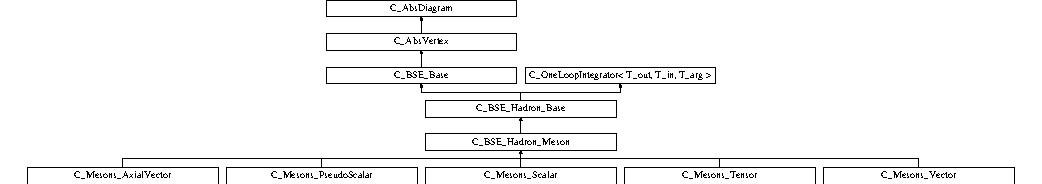
\includegraphics[height=2.470588cm]{class_c___b_s_e___hadron___meson}
\end{center}
\end{figure}
\subsection*{Public Member Functions}
\begin{DoxyCompactItemize}
\item 
\hypertarget{class_c___b_s_e___hadron___meson_ad5aac404e1c4487f905babbd03579e52}{t\-\_\-cmplx\-Matrix {\bfseries set\-Result\-B\-S\-A} ()}\label{class_c___b_s_e___hadron___meson_ad5aac404e1c4487f905babbd03579e52}

\item 
\hypertarget{class_c___b_s_e___hadron___meson_a5c4ce801dd9c216ab92b1713c6498ae7}{virtual \hyperlink{class_c___b_s_e___hadron___meson}{C\-\_\-\-B\-S\-E\-\_\-\-Hadron\-\_\-\-Meson} $\ast$ {\bfseries Make\-Copy} ()}\label{class_c___b_s_e___hadron___meson_a5c4ce801dd9c216ab92b1713c6498ae7}

\item 
\hypertarget{class_c___b_s_e___hadron___meson_a1e0d98fe901c4a1156ac98d4a6675fbd}{void {\bfseries Set\-Wave\-Functions} ()}\label{class_c___b_s_e___hadron___meson_a1e0d98fe901c4a1156ac98d4a6675fbd}

\item 
\hypertarget{class_c___b_s_e___hadron___meson_a6d1f1ba1b42166fd923b339919b93a1a}{void {\bfseries Set\-Full\-Wave\-Function} ()}\label{class_c___b_s_e___hadron___meson_a6d1f1ba1b42166fd923b339919b93a1a}

\item 
\hypertarget{class_c___b_s_e___hadron___meson_a022542fefd05923bf4654efcf48196f0}{void {\bfseries Set\-Full\-Amplitude} ()}\label{class_c___b_s_e___hadron___meson_a022542fefd05923bf4654efcf48196f0}

\item 
\hypertarget{class_c___b_s_e___hadron___meson_ab6b95e521b37c8cfae6ecae14532db88}{t\-\_\-cmplx\-Matrix {\bfseries Get\-B\-S\-A} ()}\label{class_c___b_s_e___hadron___meson_ab6b95e521b37c8cfae6ecae14532db88}

\item 
\hypertarget{class_c___b_s_e___hadron___meson_a946c1385e8cede2351691a6b4997f215}{t\-\_\-cmplx\-Matrix {\bfseries Get\-B\-S\-A\-\_\-matrix} ()}\label{class_c___b_s_e___hadron___meson_a946c1385e8cede2351691a6b4997f215}

\item 
\hypertarget{class_c___b_s_e___hadron___meson_acf3af2d05ed380d5112734d63f215325}{t\-\_\-cmplx\-Matrix {\bfseries Get\-B\-S\-A\-\_\-norm} ()}\label{class_c___b_s_e___hadron___meson_acf3af2d05ed380d5112734d63f215325}

\item 
\hypertarget{class_c___b_s_e___hadron___meson_a13e30bc9f3555e53741acd21f0bd2ce2}{virtual t\-\_\-cmplx\-Matrix {\bfseries Disentangle\-Amps} (t\-\_\-cmplx\-Matrix $\ast$pre\-\_\-result)}\label{class_c___b_s_e___hadron___meson_a13e30bc9f3555e53741acd21f0bd2ce2}

\end{DoxyCompactItemize}
\subsection*{Static Public Member Functions}
\begin{DoxyCompactItemize}
\item 
\hypertarget{class_c___b_s_e___hadron___meson_a17fb6d15d60543e1481c022b57c57251}{static \hyperlink{class_c___b_s_e___hadron___meson}{C\-\_\-\-B\-S\-E\-\_\-\-Hadron\-\_\-\-Meson} $\ast$ {\bfseries create\-Meson\-B\-S\-E} (Dirac\-\_\-\-I\-D id)}\label{class_c___b_s_e___hadron___meson_a17fb6d15d60543e1481c022b57c57251}

\end{DoxyCompactItemize}
\subsection*{Additional Inherited Members}


The documentation for this class was generated from the following file\-:\begin{DoxyCompactItemize}
\item 
source/\-Vertex/\-B\-S\-E/B\-S\-E\-\_\-\-Mesons.\-hpp\end{DoxyCompactItemize}

\hypertarget{class_c___b_s_e___hadron__parameters}{\section{C\-\_\-\-B\-S\-E\-\_\-\-Hadron\-\_\-parameters Class Reference}
\label{class_c___b_s_e___hadron__parameters}\index{C\-\_\-\-B\-S\-E\-\_\-\-Hadron\-\_\-parameters@{C\-\_\-\-B\-S\-E\-\_\-\-Hadron\-\_\-parameters}}
}
\subsection*{Public Member Functions}
\begin{DoxyCompactItemize}
\item 
\hypertarget{class_c___b_s_e___hadron__parameters_a8fbe8f04ce6ebc396e2a424ec14ed8be}{void {\bfseries Print} (std\-::ostream \&\-\_\-\-\_\-os=std\-::cout) const }\label{class_c___b_s_e___hadron__parameters_a8fbe8f04ce6ebc396e2a424ec14ed8be}

\item 
\hypertarget{class_c___b_s_e___hadron__parameters_ac1739ea129ef87c7db78f613ad6b84e2}{void {\bfseries set\-Params} (std\-::ifstream $\ast$\-\_\-\-Param\-List)}\label{class_c___b_s_e___hadron__parameters_ac1739ea129ef87c7db78f613ad6b84e2}

\end{DoxyCompactItemize}
\subsection*{Public Attributes}
\begin{DoxyCompactItemize}
\item 
\hypertarget{class_c___b_s_e___hadron__parameters_ab2451d57b0cd637078c8b69dc2b82a91}{int {\bfseries Num\-Radial}}\label{class_c___b_s_e___hadron__parameters_ab2451d57b0cd637078c8b69dc2b82a91}

\item 
\hypertarget{class_c___b_s_e___hadron__parameters_a91bdeaca141a4eb29d9747282b22772c}{int {\bfseries Num\-Cheb\-\_\-nod1}}\label{class_c___b_s_e___hadron__parameters_a91bdeaca141a4eb29d9747282b22772c}

\item 
\hypertarget{class_c___b_s_e___hadron__parameters_a8f658ab9f5d00f1c9a5b52cf073900de}{int {\bfseries Num\-Cheb\-\_\-nod2}}\label{class_c___b_s_e___hadron__parameters_a8f658ab9f5d00f1c9a5b52cf073900de}

\item 
\hypertarget{class_c___b_s_e___hadron__parameters_a7cf1bdc08ddcf3080ad39aee026892a5}{int {\bfseries Cheb\-\_\-order}}\label{class_c___b_s_e___hadron__parameters_a7cf1bdc08ddcf3080ad39aee026892a5}

\item 
\hypertarget{class_c___b_s_e___hadron__parameters_a3e131bb6cb2a68bcff572d73f4300de1}{int {\bfseries Num\-Angle\-Y}}\label{class_c___b_s_e___hadron__parameters_a3e131bb6cb2a68bcff572d73f4300de1}

\item 
\hypertarget{class_c___b_s_e___hadron__parameters_a2789774ff7116e5a2fed8fe171c9bcf1}{int {\bfseries Num\-Radial\-\_\-\-Contour}}\label{class_c___b_s_e___hadron__parameters_a2789774ff7116e5a2fed8fe171c9bcf1}

\item 
\hypertarget{class_c___b_s_e___hadron__parameters_ac94620babdbd436138c182a89f24777d}{int {\bfseries Num\-Cheb\-\_\-\-Contour}}\label{class_c___b_s_e___hadron__parameters_ac94620babdbd436138c182a89f24777d}

\item 
\hypertarget{class_c___b_s_e___hadron__parameters_aeebc2701b5f5d6c01e699735f4c3f688}{int {\bfseries Num\-Angle\-Y\-\_\-\-Contour}}\label{class_c___b_s_e___hadron__parameters_aeebc2701b5f5d6c01e699735f4c3f688}

\item 
\hypertarget{class_c___b_s_e___hadron__parameters_a588fbbfa3942530682e12a0db01c0c81}{int {\bfseries Num\-Radial\-\_\-\-Matrix}}\label{class_c___b_s_e___hadron__parameters_a588fbbfa3942530682e12a0db01c0c81}

\item 
\hypertarget{class_c___b_s_e___hadron__parameters_afa402937e179655de9ccec21b82a217a}{int {\bfseries Num\-Cheb\-\_\-\-Matrix}}\label{class_c___b_s_e___hadron__parameters_afa402937e179655de9ccec21b82a217a}

\item 
\hypertarget{class_c___b_s_e___hadron__parameters_acdac430bcba98a4ebd36125dca8e2b84}{int {\bfseries Num\-Angle\-Y\-\_\-\-Matrix}}\label{class_c___b_s_e___hadron__parameters_acdac430bcba98a4ebd36125dca8e2b84}

\item 
\hypertarget{class_c___b_s_e___hadron__parameters_a613d1099920c29bca627385d25b530df}{double {\bfseries Lim\-Uk}}\label{class_c___b_s_e___hadron__parameters_a613d1099920c29bca627385d25b530df}

\item 
\hypertarget{class_c___b_s_e___hadron__parameters_aa2e276f9dbf35b46dc7627cf3b354460}{double {\bfseries Lim\-Dk}}\label{class_c___b_s_e___hadron__parameters_aa2e276f9dbf35b46dc7627cf3b354460}

\item 
\hypertarget{class_c___b_s_e___hadron__parameters_afeb651bcc9c2086093f62adb20f15882}{double {\bfseries zetta\-\_\-part}}\label{class_c___b_s_e___hadron__parameters_afeb651bcc9c2086093f62adb20f15882}

\item 
\hypertarget{class_c___b_s_e___hadron__parameters_a56755348cb398bda3fda906396452c0b}{bool {\bfseries Off\-Shell}}\label{class_c___b_s_e___hadron__parameters_a56755348cb398bda3fda906396452c0b}

\end{DoxyCompactItemize}


The documentation for this class was generated from the following file\-:\begin{DoxyCompactItemize}
\item 
source/\-Vertex/\-B\-S\-E/B\-S\-E\-\_\-\-Base.\-hpp\end{DoxyCompactItemize}

\hypertarget{class_c___charm___quark}{\section{C\-\_\-\-Charm\-\_\-\-Quark Class Reference}
\label{class_c___charm___quark}\index{C\-\_\-\-Charm\-\_\-\-Quark@{C\-\_\-\-Charm\-\_\-\-Quark}}
}
Inheritance diagram for C\-\_\-\-Charm\-\_\-\-Quark\-:\begin{figure}[H]
\begin{center}
\leavevmode
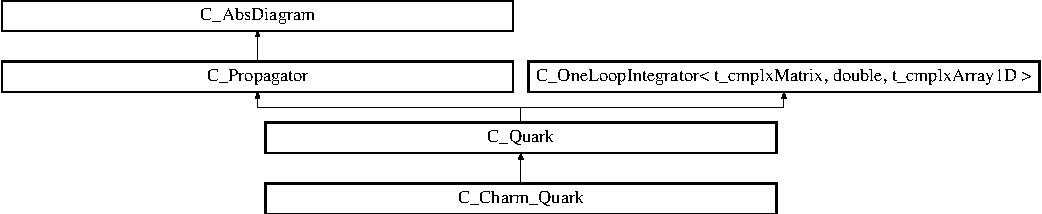
\includegraphics[height=2.871795cm]{class_c___charm___quark}
\end{center}
\end{figure}
\subsection*{Public Member Functions}
\begin{DoxyCompactItemize}
\item 
\hypertarget{class_c___charm___quark_acd91950b78021effccd54c0a60d8c697}{void {\bfseries info} ()}\label{class_c___charm___quark_acd91950b78021effccd54c0a60d8c697}

\end{DoxyCompactItemize}
\subsection*{Additional Inherited Members}


The documentation for this class was generated from the following file\-:\begin{DoxyCompactItemize}
\item 
source/\-D\-S\-E/Quark\-Types.\-hpp\end{DoxyCompactItemize}

\hypertarget{class_c___dedic_mem___abs}{\section{C\-\_\-\-Dedic\-Mem\-\_\-\-Abs Class Reference}
\label{class_c___dedic_mem___abs}\index{C\-\_\-\-Dedic\-Mem\-\_\-\-Abs@{C\-\_\-\-Dedic\-Mem\-\_\-\-Abs}}
}
Inheritance diagram for C\-\_\-\-Dedic\-Mem\-\_\-\-Abs\-:\begin{figure}[H]
\begin{center}
\leavevmode
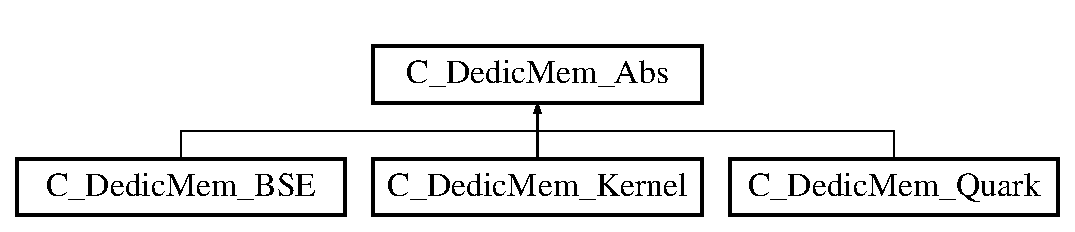
\includegraphics[height=2.000000cm]{class_c___dedic_mem___abs}
\end{center}
\end{figure}
\subsection*{Public Member Functions}
\begin{DoxyCompactItemize}
\item 
\hypertarget{class_c___dedic_mem___abs_a058cad18bf5cbc3e4d20272e41158f86}{virtual void {\bfseries info} ()=0}\label{class_c___dedic_mem___abs_a058cad18bf5cbc3e4d20272e41158f86}

\end{DoxyCompactItemize}


The documentation for this class was generated from the following file\-:\begin{DoxyCompactItemize}
\item 
source/\-Dedic\-Mem/Dedic\-Mem.\-hpp\end{DoxyCompactItemize}

\hypertarget{class_c___dedic_mem___b_s_e}{\section{C\-\_\-\-Dedic\-Mem\-\_\-\-B\-S\-E Class Reference}
\label{class_c___dedic_mem___b_s_e}\index{C\-\_\-\-Dedic\-Mem\-\_\-\-B\-S\-E@{C\-\_\-\-Dedic\-Mem\-\_\-\-B\-S\-E}}
}
Inheritance diagram for C\-\_\-\-Dedic\-Mem\-\_\-\-B\-S\-E\-:\begin{figure}[H]
\begin{center}
\leavevmode
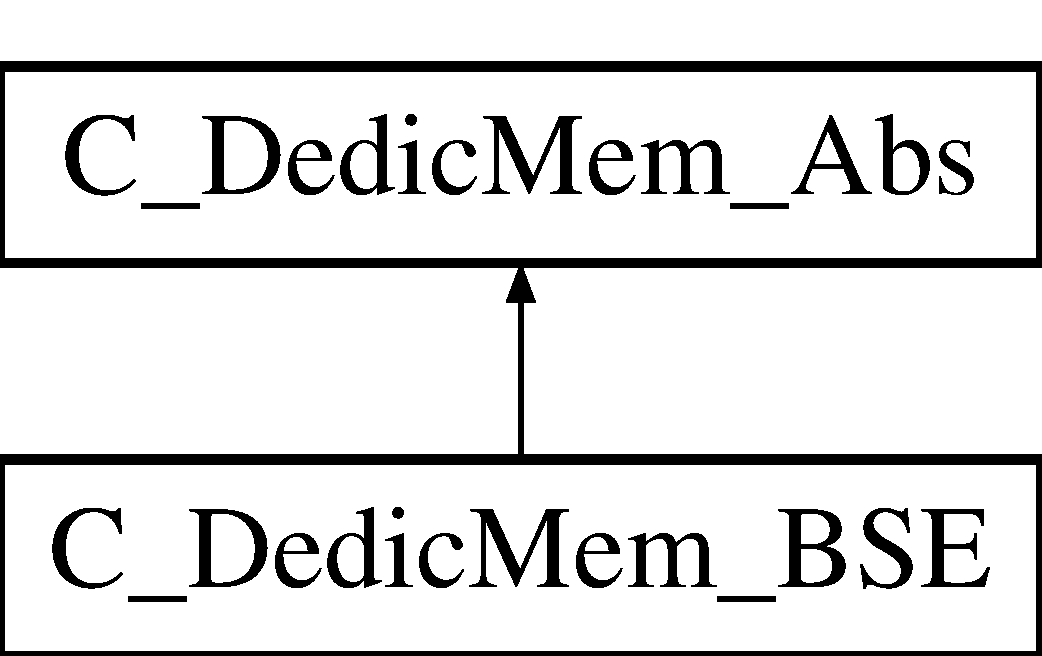
\includegraphics[height=2.000000cm]{class_c___dedic_mem___b_s_e}
\end{center}
\end{figure}
\subsection*{Public Member Functions}
\begin{DoxyCompactItemize}
\item 
\hypertarget{class_c___dedic_mem___b_s_e_ad6928f35d1bb6dc0a9e7896cb435de77}{void {\bfseries resize\-Amp\-Storage} (int amps, int points)}\label{class_c___dedic_mem___b_s_e_ad6928f35d1bb6dc0a9e7896cb435de77}

\item 
\hypertarget{class_c___dedic_mem___b_s_e_ae0fc9faee6bf0212366e272929d05299}{void {\bfseries set\-Amp\-Storage} (int amp, int point, t\-\_\-cmplx\-Dirac $\ast$Amp)}\label{class_c___dedic_mem___b_s_e_ae0fc9faee6bf0212366e272929d05299}

\item 
\hypertarget{class_c___dedic_mem___b_s_e_a1e45518a37fafeb43d866fdf8b60dbd6}{t\-\_\-cmplx\-Dirac {\bfseries get\-Amp\-Storage} (int amp, int point)}\label{class_c___dedic_mem___b_s_e_a1e45518a37fafeb43d866fdf8b60dbd6}

\item 
\hypertarget{class_c___dedic_mem___b_s_e_a832e259d5897e9b274d529979d92d08f}{void {\bfseries clear\-Amp\-Storage} ()}\label{class_c___dedic_mem___b_s_e_a832e259d5897e9b274d529979d92d08f}

\item 
\hypertarget{class_c___dedic_mem___b_s_e_a4e6c97cc94e185ccb93b4b83a6caa986}{void {\bfseries Resize\-E\-V\-Matrix} (int num\-\_\-rad, int num\-\_\-angle, int num\-\_\-amplitudes, int num\-\_\-chebs)}\label{class_c___dedic_mem___b_s_e_a4e6c97cc94e185ccb93b4b83a6caa986}

\item 
\hypertarget{class_c___dedic_mem___b_s_e_a77dd95cd06387357599deb84c8a1b5f3}{void {\bfseries resize\-B\-S\-E\-Contour} (int num\-\_\-amplitudes, int num\-\_\-points)}\label{class_c___dedic_mem___b_s_e_a77dd95cd06387357599deb84c8a1b5f3}

\item 
\hypertarget{class_c___dedic_mem___b_s_e_a1acb22de1a69296a075dc76a066c1cff}{void {\bfseries resize\-B\-S\-E\-Grid} (int num\-\_\-amplitudes, int num\-\_\-ex, int num\-\_\-in)}\label{class_c___dedic_mem___b_s_e_a1acb22de1a69296a075dc76a066c1cff}

\item 
\hypertarget{class_c___dedic_mem___b_s_e_a8eb9828cf1137c08d65e9c531f57dd87}{void {\bfseries clear\-Cauchy\-Grid} ()}\label{class_c___dedic_mem___b_s_e_a8eb9828cf1137c08d65e9c531f57dd87}

\item 
\hypertarget{class_c___dedic_mem___b_s_e_a7db75e75c587b9a25e937bb77ee399d7}{void {\bfseries info} ()}\label{class_c___dedic_mem___b_s_e_a7db75e75c587b9a25e937bb77ee399d7}

\end{DoxyCompactItemize}
\subsection*{Public Attributes}
\begin{DoxyCompactItemize}
\item 
\hypertarget{class_c___dedic_mem___b_s_e_a532449af372b4823ec11c1bac16a39f6}{std\-::vector$<$ std\-::vector\\*
$<$ t\-\_\-cmplx\-Dirac $>$ $>$ {\bfseries Amp\-Storage}}\label{class_c___dedic_mem___b_s_e_a532449af372b4823ec11c1bac16a39f6}

\item 
\hypertarget{class_c___dedic_mem___b_s_e_a5f0de44c8872d59b5db86058088e040e}{Eigen\-::\-Matrix\-Xcf {\bfseries E\-V\-Matrix}}\label{class_c___dedic_mem___b_s_e_a5f0de44c8872d59b5db86058088e040e}

\item 
\hypertarget{class_c___dedic_mem___b_s_e_adcbf7c4206df13acafeab297bc039f29}{t\-\_\-cmplx\-Array2\-D {\bfseries Cauchy\-Contour}}\label{class_c___dedic_mem___b_s_e_adcbf7c4206df13acafeab297bc039f29}

\item 
\hypertarget{class_c___dedic_mem___b_s_e_a0d11282e491e4762101a83d7e80e5733}{t\-\_\-cmplx\-Array3\-D {\bfseries Cauchy\-Grid}}\label{class_c___dedic_mem___b_s_e_a0d11282e491e4762101a83d7e80e5733}

\end{DoxyCompactItemize}


The documentation for this class was generated from the following files\-:\begin{DoxyCompactItemize}
\item 
source/\-Dedic\-Mem/Dedic\-Mem.\-hpp\item 
source/\-Dedic\-Mem/Dedic\-Mem.\-cpp\end{DoxyCompactItemize}

\hypertarget{class_c___dedic_mem___kernel}{\section{C\-\_\-\-Dedic\-Mem\-\_\-\-Kernel Class Reference}
\label{class_c___dedic_mem___kernel}\index{C\-\_\-\-Dedic\-Mem\-\_\-\-Kernel@{C\-\_\-\-Dedic\-Mem\-\_\-\-Kernel}}
}


{\ttfamily \#include $<$Dedic\-Mem.\-hpp$>$}

Inheritance diagram for C\-\_\-\-Dedic\-Mem\-\_\-\-Kernel\-:\begin{figure}[H]
\begin{center}
\leavevmode
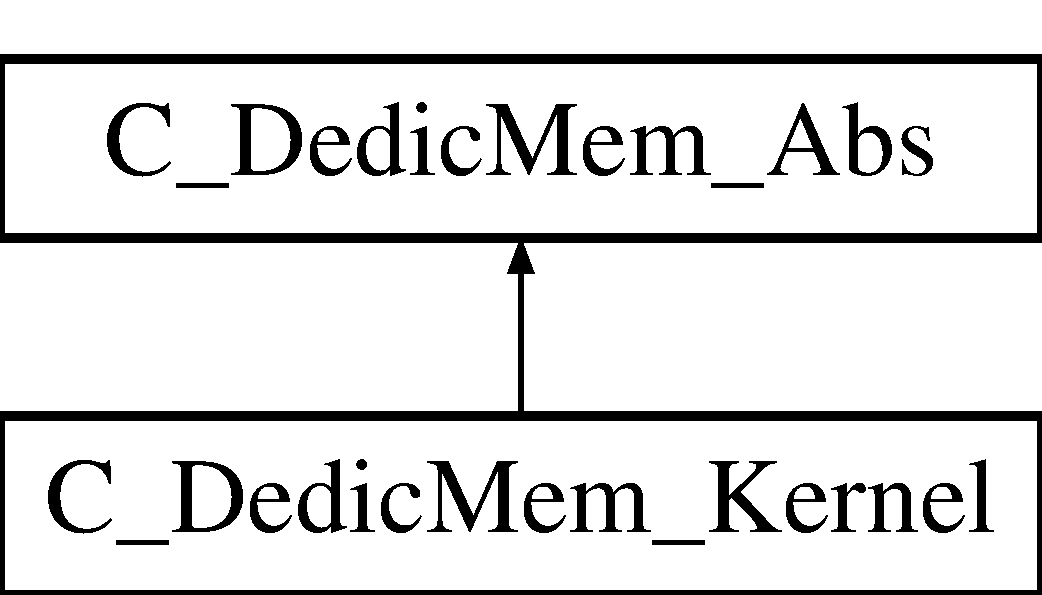
\includegraphics[height=2.000000cm]{class_c___dedic_mem___kernel}
\end{center}
\end{figure}
\subsection*{Public Member Functions}
\begin{DoxyCompactItemize}
\item 
void \hyperlink{class_c___dedic_mem___kernel_aa51b1668792ba7e0f843b2d03deb5819}{info} ()
\item 
void \hyperlink{class_c___dedic_mem___kernel_a53112d51dde01d8b4bd8f48ccce36a91}{Resize\-Kstorage} (int i)
\item 
void \hyperlink{class_c___dedic_mem___kernel_ac2013ecffb5dab674a568ef256f5a3f8}{Set\-Kmatrix\-At} (int i, \hyperlink{types_8h_ab0ebabce2061a9cbb83363a282add98f}{t\-\_\-cmplx\-Matrix2\-D} $\ast$\-\_\-\-K)
\item 
void \hyperlink{class_c___dedic_mem___kernel_ae8436015627826c00ef38c038ef829f8}{Erase\-Kstorage} ()
\item 
\hyperlink{types_8h_ab0ebabce2061a9cbb83363a282add98f}{t\-\_\-cmplx\-Matrix2\-D} $\ast$ \hyperlink{class_c___dedic_mem___kernel_aa95a927579efd2c095634e813c0db40f}{Get\-Kmatrix\-At} (int i)
\end{DoxyCompactItemize}
\subsection*{Public Attributes}
\begin{DoxyCompactItemize}
\item 
\hyperlink{types_8h_a71e866ee00a3173697327849014bce9b}{t\-\_\-cmplx\-Array4\-D} \hyperlink{class_c___dedic_mem___kernel_a1b2fcfb12ebf53baed1105d05c61f5fb}{Vertex\-Dressings}
\end{DoxyCompactItemize}


\subsection{Member Function Documentation}
\hypertarget{class_c___dedic_mem___kernel_ae8436015627826c00ef38c038ef829f8}{\index{C\-\_\-\-Dedic\-Mem\-\_\-\-Kernel@{C\-\_\-\-Dedic\-Mem\-\_\-\-Kernel}!Erase\-Kstorage@{Erase\-Kstorage}}
\index{Erase\-Kstorage@{Erase\-Kstorage}!C_DedicMem_Kernel@{C\-\_\-\-Dedic\-Mem\-\_\-\-Kernel}}
\subsubsection[{Erase\-Kstorage}]{\setlength{\rightskip}{0pt plus 5cm}void C\-\_\-\-Dedic\-Mem\-\_\-\-Kernel\-::\-Erase\-Kstorage (
\begin{DoxyParamCaption}
{}
\end{DoxyParamCaption}
)}}\label{class_c___dedic_mem___kernel_ae8436015627826c00ef38c038ef829f8}
\hypertarget{class_c___dedic_mem___kernel_aa95a927579efd2c095634e813c0db40f}{\index{C\-\_\-\-Dedic\-Mem\-\_\-\-Kernel@{C\-\_\-\-Dedic\-Mem\-\_\-\-Kernel}!Get\-Kmatrix\-At@{Get\-Kmatrix\-At}}
\index{Get\-Kmatrix\-At@{Get\-Kmatrix\-At}!C_DedicMem_Kernel@{C\-\_\-\-Dedic\-Mem\-\_\-\-Kernel}}
\subsubsection[{Get\-Kmatrix\-At}]{\setlength{\rightskip}{0pt plus 5cm}{\bf t\-\_\-cmplx\-Matrix2\-D} $\ast$ C\-\_\-\-Dedic\-Mem\-\_\-\-Kernel\-::\-Get\-Kmatrix\-At (
\begin{DoxyParamCaption}
\item[{int}]{i}
\end{DoxyParamCaption}
)}}\label{class_c___dedic_mem___kernel_aa95a927579efd2c095634e813c0db40f}
\hypertarget{class_c___dedic_mem___kernel_aa51b1668792ba7e0f843b2d03deb5819}{\index{C\-\_\-\-Dedic\-Mem\-\_\-\-Kernel@{C\-\_\-\-Dedic\-Mem\-\_\-\-Kernel}!info@{info}}
\index{info@{info}!C_DedicMem_Kernel@{C\-\_\-\-Dedic\-Mem\-\_\-\-Kernel}}
\subsubsection[{info}]{\setlength{\rightskip}{0pt plus 5cm}void C\-\_\-\-Dedic\-Mem\-\_\-\-Kernel\-::info (
\begin{DoxyParamCaption}
{}
\end{DoxyParamCaption}
)\hspace{0.3cm}{\ttfamily [virtual]}}}\label{class_c___dedic_mem___kernel_aa51b1668792ba7e0f843b2d03deb5819}


Implements \hyperlink{class_c___dedic_mem___abs_a058cad18bf5cbc3e4d20272e41158f86}{C\-\_\-\-Dedic\-Mem\-\_\-\-Abs}.

\hypertarget{class_c___dedic_mem___kernel_a53112d51dde01d8b4bd8f48ccce36a91}{\index{C\-\_\-\-Dedic\-Mem\-\_\-\-Kernel@{C\-\_\-\-Dedic\-Mem\-\_\-\-Kernel}!Resize\-Kstorage@{Resize\-Kstorage}}
\index{Resize\-Kstorage@{Resize\-Kstorage}!C_DedicMem_Kernel@{C\-\_\-\-Dedic\-Mem\-\_\-\-Kernel}}
\subsubsection[{Resize\-Kstorage}]{\setlength{\rightskip}{0pt plus 5cm}void C\-\_\-\-Dedic\-Mem\-\_\-\-Kernel\-::\-Resize\-Kstorage (
\begin{DoxyParamCaption}
\item[{int}]{i}
\end{DoxyParamCaption}
)}}\label{class_c___dedic_mem___kernel_a53112d51dde01d8b4bd8f48ccce36a91}
\hypertarget{class_c___dedic_mem___kernel_ac2013ecffb5dab674a568ef256f5a3f8}{\index{C\-\_\-\-Dedic\-Mem\-\_\-\-Kernel@{C\-\_\-\-Dedic\-Mem\-\_\-\-Kernel}!Set\-Kmatrix\-At@{Set\-Kmatrix\-At}}
\index{Set\-Kmatrix\-At@{Set\-Kmatrix\-At}!C_DedicMem_Kernel@{C\-\_\-\-Dedic\-Mem\-\_\-\-Kernel}}
\subsubsection[{Set\-Kmatrix\-At}]{\setlength{\rightskip}{0pt plus 5cm}void C\-\_\-\-Dedic\-Mem\-\_\-\-Kernel\-::\-Set\-Kmatrix\-At (
\begin{DoxyParamCaption}
\item[{int}]{i, }
\item[{{\bf t\-\_\-cmplx\-Matrix2\-D} $\ast$}]{\-\_\-\-K}
\end{DoxyParamCaption}
)}}\label{class_c___dedic_mem___kernel_ac2013ecffb5dab674a568ef256f5a3f8}


\subsection{Member Data Documentation}
\hypertarget{class_c___dedic_mem___kernel_a1b2fcfb12ebf53baed1105d05c61f5fb}{\index{C\-\_\-\-Dedic\-Mem\-\_\-\-Kernel@{C\-\_\-\-Dedic\-Mem\-\_\-\-Kernel}!Vertex\-Dressings@{Vertex\-Dressings}}
\index{Vertex\-Dressings@{Vertex\-Dressings}!C_DedicMem_Kernel@{C\-\_\-\-Dedic\-Mem\-\_\-\-Kernel}}
\subsubsection[{Vertex\-Dressings}]{\setlength{\rightskip}{0pt plus 5cm}{\bf t\-\_\-cmplx\-Array4\-D} C\-\_\-\-Dedic\-Mem\-\_\-\-Kernel\-::\-Vertex\-Dressings}}\label{class_c___dedic_mem___kernel_a1b2fcfb12ebf53baed1105d05c61f5fb}


The documentation for this class was generated from the following files\-:\begin{DoxyCompactItemize}
\item 
source/\-Dedic\-Mem/\hyperlink{_dedic_mem_8hpp}{Dedic\-Mem.\-hpp}\item 
source/\-Dedic\-Mem/\hyperlink{_dedic_mem_8cpp}{Dedic\-Mem.\-cpp}\end{DoxyCompactItemize}

\hypertarget{class_c___dedic_mem___quark}{\section{C\-\_\-\-Dedic\-Mem\-\_\-\-Quark Class Reference}
\label{class_c___dedic_mem___quark}\index{C\-\_\-\-Dedic\-Mem\-\_\-\-Quark@{C\-\_\-\-Dedic\-Mem\-\_\-\-Quark}}
}


{\ttfamily \#include $<$Dedic\-Mem.\-hpp$>$}

Inheritance diagram for C\-\_\-\-Dedic\-Mem\-\_\-\-Quark\-:\begin{figure}[H]
\begin{center}
\leavevmode
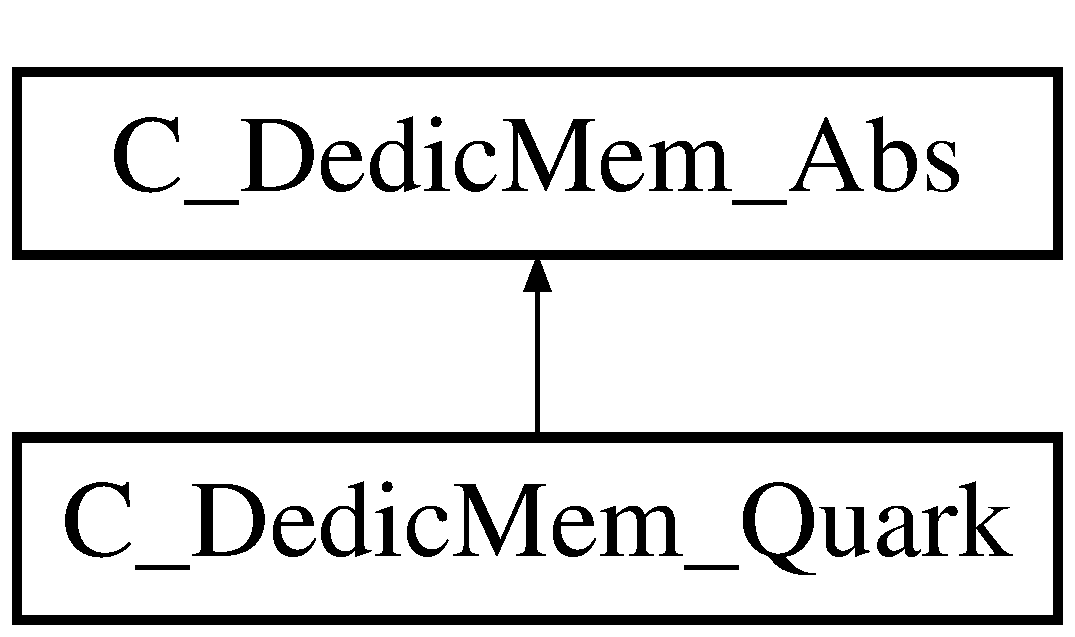
\includegraphics[height=2.000000cm]{class_c___dedic_mem___quark}
\end{center}
\end{figure}
\subsection*{Public Member Functions}
\begin{DoxyCompactItemize}
\item 
void \hyperlink{class_c___dedic_mem___quark_af9870170bb87b11db976c64fa2ff87bb}{resize\-Grid} (int amps\-\_\-num, int exter\-\_\-num, int inter\-\_\-num)
\item 
void \hyperlink{class_c___dedic_mem___quark_af25f857d41fa0b568af4a11218580729}{resize\-Contour} (int amps\-\_\-num, int cont\-\_\-num)
\item 
void \hyperlink{class_c___dedic_mem___quark_a868c98c7d5930a7fd0b4314d79092581}{Remove\-Grid} ()
\item 
void \hyperlink{class_c___dedic_mem___quark_aa2c1bd42ef41a11746d8ab96dcc70e75}{Remove\-Contour} ()
\item 
void \hyperlink{class_c___dedic_mem___quark_a7252d680bbd53e5c9a183fa49117d2e3}{info} ()
\end{DoxyCompactItemize}
\subsection*{Public Attributes}
\begin{DoxyCompactItemize}
\item 
\hyperlink{types_8h_a13088102853997a3c148dfe29c372f85}{t\-\_\-cmplx\-Array3\-D} \hyperlink{class_c___dedic_mem___quark_abb615a8d4eb2c5844634ac810197ad61}{S\-\_\-grid}
\item 
\hyperlink{types_8h_a4db8c78f1689c3a957b2866daaae58f2}{t\-\_\-cmplx\-Array2\-D} \hyperlink{class_c___dedic_mem___quark_a211eb01b6fb3e276987b2a99899d18b6}{S\-\_\-cont}
\end{DoxyCompactItemize}


\subsection{Member Function Documentation}
\hypertarget{class_c___dedic_mem___quark_a7252d680bbd53e5c9a183fa49117d2e3}{\index{C\-\_\-\-Dedic\-Mem\-\_\-\-Quark@{C\-\_\-\-Dedic\-Mem\-\_\-\-Quark}!info@{info}}
\index{info@{info}!C_DedicMem_Quark@{C\-\_\-\-Dedic\-Mem\-\_\-\-Quark}}
\subsubsection[{info}]{\setlength{\rightskip}{0pt plus 5cm}void C\-\_\-\-Dedic\-Mem\-\_\-\-Quark\-::info (
\begin{DoxyParamCaption}
{}
\end{DoxyParamCaption}
)\hspace{0.3cm}{\ttfamily [virtual]}}}\label{class_c___dedic_mem___quark_a7252d680bbd53e5c9a183fa49117d2e3}


Implements \hyperlink{class_c___dedic_mem___abs_a058cad18bf5cbc3e4d20272e41158f86}{C\-\_\-\-Dedic\-Mem\-\_\-\-Abs}.

\hypertarget{class_c___dedic_mem___quark_aa2c1bd42ef41a11746d8ab96dcc70e75}{\index{C\-\_\-\-Dedic\-Mem\-\_\-\-Quark@{C\-\_\-\-Dedic\-Mem\-\_\-\-Quark}!Remove\-Contour@{Remove\-Contour}}
\index{Remove\-Contour@{Remove\-Contour}!C_DedicMem_Quark@{C\-\_\-\-Dedic\-Mem\-\_\-\-Quark}}
\subsubsection[{Remove\-Contour}]{\setlength{\rightskip}{0pt plus 5cm}void C\-\_\-\-Dedic\-Mem\-\_\-\-Quark\-::\-Remove\-Contour (
\begin{DoxyParamCaption}
{}
\end{DoxyParamCaption}
)}}\label{class_c___dedic_mem___quark_aa2c1bd42ef41a11746d8ab96dcc70e75}
\hypertarget{class_c___dedic_mem___quark_a868c98c7d5930a7fd0b4314d79092581}{\index{C\-\_\-\-Dedic\-Mem\-\_\-\-Quark@{C\-\_\-\-Dedic\-Mem\-\_\-\-Quark}!Remove\-Grid@{Remove\-Grid}}
\index{Remove\-Grid@{Remove\-Grid}!C_DedicMem_Quark@{C\-\_\-\-Dedic\-Mem\-\_\-\-Quark}}
\subsubsection[{Remove\-Grid}]{\setlength{\rightskip}{0pt plus 5cm}void C\-\_\-\-Dedic\-Mem\-\_\-\-Quark\-::\-Remove\-Grid (
\begin{DoxyParamCaption}
{}
\end{DoxyParamCaption}
)}}\label{class_c___dedic_mem___quark_a868c98c7d5930a7fd0b4314d79092581}
\hypertarget{class_c___dedic_mem___quark_af25f857d41fa0b568af4a11218580729}{\index{C\-\_\-\-Dedic\-Mem\-\_\-\-Quark@{C\-\_\-\-Dedic\-Mem\-\_\-\-Quark}!resize\-Contour@{resize\-Contour}}
\index{resize\-Contour@{resize\-Contour}!C_DedicMem_Quark@{C\-\_\-\-Dedic\-Mem\-\_\-\-Quark}}
\subsubsection[{resize\-Contour}]{\setlength{\rightskip}{0pt plus 5cm}void C\-\_\-\-Dedic\-Mem\-\_\-\-Quark\-::resize\-Contour (
\begin{DoxyParamCaption}
\item[{int}]{amps\-\_\-num, }
\item[{int}]{cont\-\_\-num}
\end{DoxyParamCaption}
)}}\label{class_c___dedic_mem___quark_af25f857d41fa0b568af4a11218580729}
\hypertarget{class_c___dedic_mem___quark_af9870170bb87b11db976c64fa2ff87bb}{\index{C\-\_\-\-Dedic\-Mem\-\_\-\-Quark@{C\-\_\-\-Dedic\-Mem\-\_\-\-Quark}!resize\-Grid@{resize\-Grid}}
\index{resize\-Grid@{resize\-Grid}!C_DedicMem_Quark@{C\-\_\-\-Dedic\-Mem\-\_\-\-Quark}}
\subsubsection[{resize\-Grid}]{\setlength{\rightskip}{0pt plus 5cm}void C\-\_\-\-Dedic\-Mem\-\_\-\-Quark\-::resize\-Grid (
\begin{DoxyParamCaption}
\item[{int}]{amps\-\_\-num, }
\item[{int}]{exter\-\_\-num, }
\item[{int}]{inter\-\_\-num}
\end{DoxyParamCaption}
)}}\label{class_c___dedic_mem___quark_af9870170bb87b11db976c64fa2ff87bb}


\subsection{Member Data Documentation}
\hypertarget{class_c___dedic_mem___quark_a211eb01b6fb3e276987b2a99899d18b6}{\index{C\-\_\-\-Dedic\-Mem\-\_\-\-Quark@{C\-\_\-\-Dedic\-Mem\-\_\-\-Quark}!S\-\_\-cont@{S\-\_\-cont}}
\index{S\-\_\-cont@{S\-\_\-cont}!C_DedicMem_Quark@{C\-\_\-\-Dedic\-Mem\-\_\-\-Quark}}
\subsubsection[{S\-\_\-cont}]{\setlength{\rightskip}{0pt plus 5cm}{\bf t\-\_\-cmplx\-Array2\-D} C\-\_\-\-Dedic\-Mem\-\_\-\-Quark\-::\-S\-\_\-cont}}\label{class_c___dedic_mem___quark_a211eb01b6fb3e276987b2a99899d18b6}
\hypertarget{class_c___dedic_mem___quark_abb615a8d4eb2c5844634ac810197ad61}{\index{C\-\_\-\-Dedic\-Mem\-\_\-\-Quark@{C\-\_\-\-Dedic\-Mem\-\_\-\-Quark}!S\-\_\-grid@{S\-\_\-grid}}
\index{S\-\_\-grid@{S\-\_\-grid}!C_DedicMem_Quark@{C\-\_\-\-Dedic\-Mem\-\_\-\-Quark}}
\subsubsection[{S\-\_\-grid}]{\setlength{\rightskip}{0pt plus 5cm}{\bf t\-\_\-cmplx\-Array3\-D} C\-\_\-\-Dedic\-Mem\-\_\-\-Quark\-::\-S\-\_\-grid}}\label{class_c___dedic_mem___quark_abb615a8d4eb2c5844634ac810197ad61}


The documentation for this class was generated from the following files\-:\begin{DoxyCompactItemize}
\item 
source/\-Dedic\-Mem/\hyperlink{_dedic_mem_8hpp}{Dedic\-Mem.\-hpp}\item 
source/\-Dedic\-Mem/\hyperlink{_dedic_mem_8cpp}{Dedic\-Mem.\-cpp}\end{DoxyCompactItemize}

\hypertarget{class_c___down___quark}{\section{C\-\_\-\-Down\-\_\-\-Quark Class Reference}
\label{class_c___down___quark}\index{C\-\_\-\-Down\-\_\-\-Quark@{C\-\_\-\-Down\-\_\-\-Quark}}
}
Inheritance diagram for C\-\_\-\-Down\-\_\-\-Quark\-:\begin{figure}[H]
\begin{center}
\leavevmode
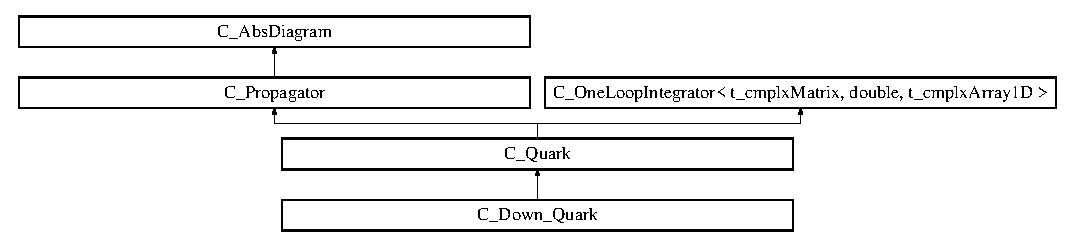
\includegraphics[height=2.871795cm]{class_c___down___quark}
\end{center}
\end{figure}
\subsection*{Public Member Functions}
\begin{DoxyCompactItemize}
\item 
\hypertarget{class_c___down___quark_a24efadd8c5e082d85b02e376f08bf6cc}{void {\bfseries info} ()}\label{class_c___down___quark_a24efadd8c5e082d85b02e376f08bf6cc}

\end{DoxyCompactItemize}
\subsection*{Additional Inherited Members}


The documentation for this class was generated from the following file\-:\begin{DoxyCompactItemize}
\item 
source/\-D\-S\-E/Quark\-Types.\-hpp\end{DoxyCompactItemize}

\hypertarget{class_c___gluon}{\section{C\-\_\-\-Gluon Class Reference}
\label{class_c___gluon}\index{C\-\_\-\-Gluon@{C\-\_\-\-Gluon}}
}


The Gluon model Although the gluon itself can posses its own D\-S\-E here we use an approximation\-: the effective gluon dressing function given by Maris-\/\-Tandy model. However any another model can be leaded from file.  




{\ttfamily \#include $<$Gluon.\-hpp$>$}

Inheritance diagram for C\-\_\-\-Gluon\-:\begin{figure}[H]
\begin{center}
\leavevmode
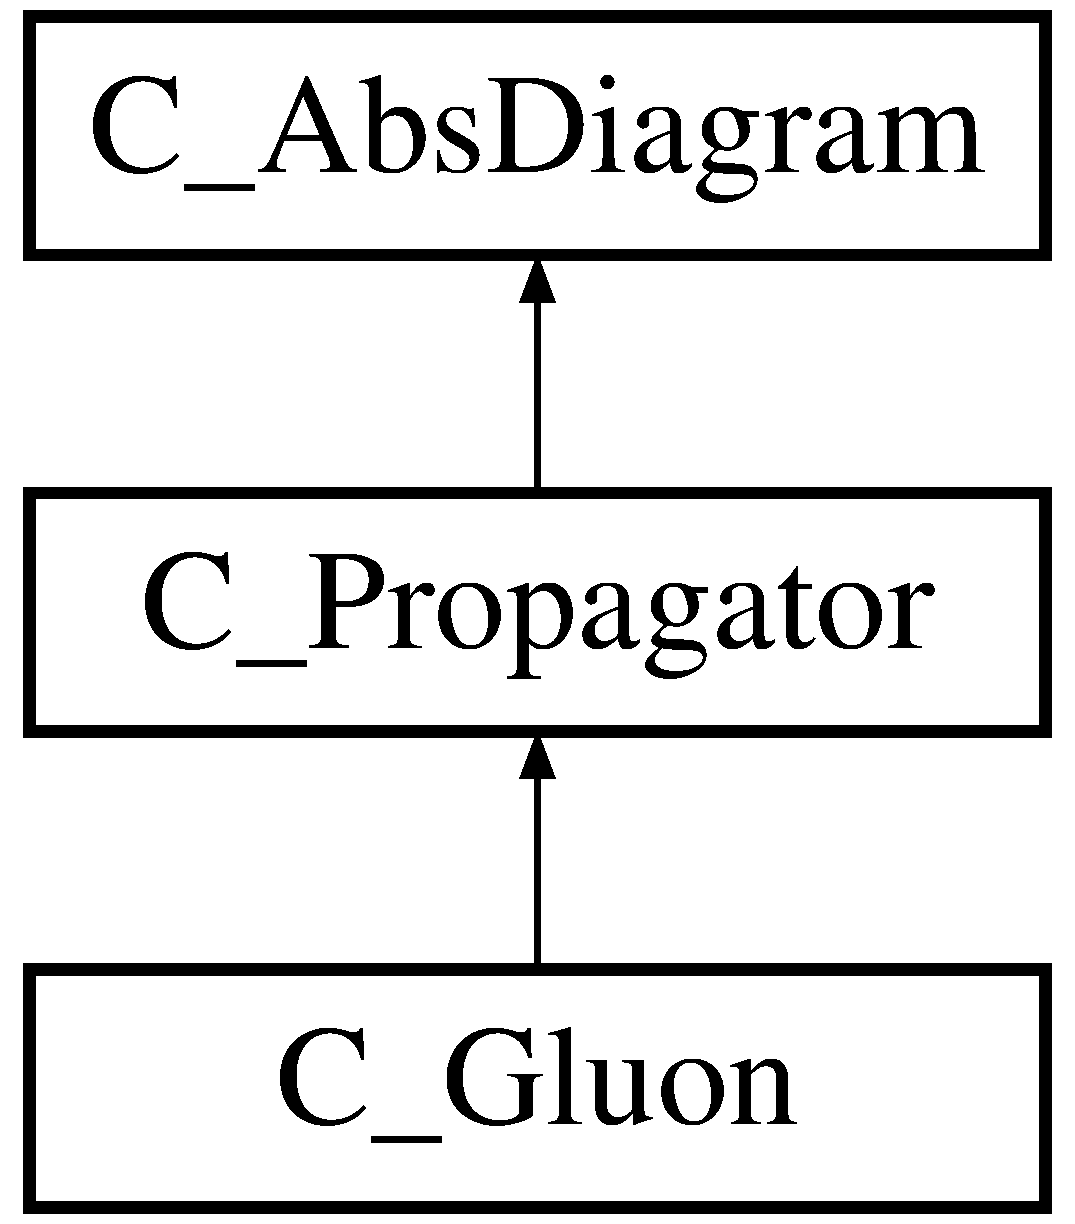
\includegraphics[height=3.000000cm]{class_c___gluon}
\end{center}
\end{figure}
\subsection*{Public Member Functions}
\begin{DoxyCompactItemize}
\item 
void \hyperlink{class_c___gluon_a44b5ce943df3ea75d258a68b1c82d865}{dress\-Propagator} ()
\item 
\hyperlink{types_8h_aab52f79903881ec15d289b3dbfb102fd}{t\-\_\-cmplx\-Array1\-D} \hyperlink{class_c___gluon_abfa90c782397bcb81c98529d46dc081f}{Propagator\-At\-Point} (\hyperlink{types_8h_aa75ae339052372f671bb263e6a272e82}{t\-\_\-cmplx} k)
\begin{DoxyCompactList}\small\item\em Get value of Gluon at /f\$ k$^\wedge$2 /f\$. \end{DoxyCompactList}\item 
void \hyperlink{class_c___gluon_a2a2f857431b7a3cb1142631d31507091}{set\-M\-T\-Params} (double Lambda, double Etta)
\begin{DoxyCompactList}\small\item\em Set manually Maris-\/\-Tandy gluon model parameters (redefined by Lambda and Etta) \end{DoxyCompactList}\end{DoxyCompactItemize}
\subsection*{Static Public Member Functions}
\begin{DoxyCompactItemize}
\item 
static \hyperlink{class_c___gluon}{C\-\_\-\-Gluon} $\ast$ \hyperlink{class_c___gluon_aa6b6cb7bfb183bfae684fa6a840643ff}{create\-Gluon} (\hyperlink{_gluon_8hpp_ac213626e6f11004cbe4bcd55fd546496}{Gluon\-\_\-\-I\-D} id)
\begin{DoxyCompactList}\small\item\em Parametrized Factory Method function. \end{DoxyCompactList}\item 
static \hyperlink{class_c___gluon}{C\-\_\-\-Gluon} $\ast$ \hyperlink{class_c___gluon_a1fa97ddd62ec8725c5c4d1c83aac3d5e}{create\-Gluon} (\hyperlink{_gluon_8hpp_ac213626e6f11004cbe4bcd55fd546496}{Gluon\-\_\-\-I\-D} id, std\-::string \&\-\_\-\-Interpolation\-Points\-Path)
\end{DoxyCompactItemize}
\subsection*{Additional Inherited Members}


\subsection{Detailed Description}
The Gluon model Although the gluon itself can posses its own D\-S\-E here we use an approximation\-: the effective gluon dressing function given by Maris-\/\-Tandy model. However any another model can be leaded from file. 

\subsection{Member Function Documentation}
\hypertarget{class_c___gluon_aa6b6cb7bfb183bfae684fa6a840643ff}{\index{C\-\_\-\-Gluon@{C\-\_\-\-Gluon}!create\-Gluon@{create\-Gluon}}
\index{create\-Gluon@{create\-Gluon}!C_Gluon@{C\-\_\-\-Gluon}}
\subsubsection[{create\-Gluon}]{\setlength{\rightskip}{0pt plus 5cm}{\bf C\-\_\-\-Gluon} $\ast$ C\-\_\-\-Gluon\-::create\-Gluon (
\begin{DoxyParamCaption}
\item[{{\bf Gluon\-\_\-\-I\-D}}]{id}
\end{DoxyParamCaption}
)\hspace{0.3cm}{\ttfamily [static]}}}\label{class_c___gluon_aa6b6cb7bfb183bfae684fa6a840643ff}


Parametrized Factory Method function. 

\hypertarget{class_c___gluon_a1fa97ddd62ec8725c5c4d1c83aac3d5e}{\index{C\-\_\-\-Gluon@{C\-\_\-\-Gluon}!create\-Gluon@{create\-Gluon}}
\index{create\-Gluon@{create\-Gluon}!C_Gluon@{C\-\_\-\-Gluon}}
\subsubsection[{create\-Gluon}]{\setlength{\rightskip}{0pt plus 5cm}{\bf C\-\_\-\-Gluon} $\ast$ C\-\_\-\-Gluon\-::create\-Gluon (
\begin{DoxyParamCaption}
\item[{{\bf Gluon\-\_\-\-I\-D}}]{id, }
\item[{std\-::string \&}]{\-\_\-\-Interpolation\-Points\-Path}
\end{DoxyParamCaption}
)\hspace{0.3cm}{\ttfamily [static]}}}\label{class_c___gluon_a1fa97ddd62ec8725c5c4d1c83aac3d5e}
\hypertarget{class_c___gluon_a44b5ce943df3ea75d258a68b1c82d865}{\index{C\-\_\-\-Gluon@{C\-\_\-\-Gluon}!dress\-Propagator@{dress\-Propagator}}
\index{dress\-Propagator@{dress\-Propagator}!C_Gluon@{C\-\_\-\-Gluon}}
\subsubsection[{dress\-Propagator}]{\setlength{\rightskip}{0pt plus 5cm}void C\-\_\-\-Gluon\-::dress\-Propagator (
\begin{DoxyParamCaption}
{}
\end{DoxyParamCaption}
)\hspace{0.3cm}{\ttfamily [inline]}, {\ttfamily [virtual]}}}\label{class_c___gluon_a44b5ce943df3ea75d258a68b1c82d865}
Dress Propagator according to defined in derived class D\-S\-E scheme this is the function where all !!\-S\-C\-I\-E\-N\-C\-E!! of D\-S\-E happens 

Implements \hyperlink{class_c___propagator_a4b82db59060878e794c3590ee3fbc3f1}{C\-\_\-\-Propagator}.

\hypertarget{class_c___gluon_abfa90c782397bcb81c98529d46dc081f}{\index{C\-\_\-\-Gluon@{C\-\_\-\-Gluon}!Propagator\-At\-Point@{Propagator\-At\-Point}}
\index{Propagator\-At\-Point@{Propagator\-At\-Point}!C_Gluon@{C\-\_\-\-Gluon}}
\subsubsection[{Propagator\-At\-Point}]{\setlength{\rightskip}{0pt plus 5cm}{\bf t\-\_\-cmplx\-Array1\-D} C\-\_\-\-Gluon\-::\-Propagator\-At\-Point (
\begin{DoxyParamCaption}
\item[{{\bf t\-\_\-cmplx}}]{k}
\end{DoxyParamCaption}
)\hspace{0.3cm}{\ttfamily [virtual]}}}\label{class_c___gluon_abfa90c782397bcb81c98529d46dc081f}


Get value of Gluon at /f\$ k$^\wedge$2 /f\$. 



Reimplemented from \hyperlink{class_c___propagator_a7bf057f408c2a30667fffea12d1375ba}{C\-\_\-\-Propagator}.

\hypertarget{class_c___gluon_a2a2f857431b7a3cb1142631d31507091}{\index{C\-\_\-\-Gluon@{C\-\_\-\-Gluon}!set\-M\-T\-Params@{set\-M\-T\-Params}}
\index{set\-M\-T\-Params@{set\-M\-T\-Params}!C_Gluon@{C\-\_\-\-Gluon}}
\subsubsection[{set\-M\-T\-Params}]{\setlength{\rightskip}{0pt plus 5cm}void C\-\_\-\-Gluon\-::set\-M\-T\-Params (
\begin{DoxyParamCaption}
\item[{double}]{Lambda, }
\item[{double}]{Etta}
\end{DoxyParamCaption}
)}}\label{class_c___gluon_a2a2f857431b7a3cb1142631d31507091}


Set manually Maris-\/\-Tandy gluon model parameters (redefined by Lambda and Etta) 



The documentation for this class was generated from the following files\-:\begin{DoxyCompactItemize}
\item 
source/\-D\-S\-E/\hyperlink{_gluon_8hpp}{Gluon.\-hpp}\item 
source/\-D\-S\-E/\hyperlink{_gluon_8cpp}{Gluon.\-cpp}\end{DoxyCompactItemize}

\hypertarget{class_c___gluon___factory}{\section{C\-\_\-\-Gluon\-\_\-\-Factory Class Reference}
\label{class_c___gluon___factory}\index{C\-\_\-\-Gluon\-\_\-\-Factory@{C\-\_\-\-Gluon\-\_\-\-Factory}}
}
Inheritance diagram for C\-\_\-\-Gluon\-\_\-\-Factory\-:\begin{figure}[H]
\begin{center}
\leavevmode
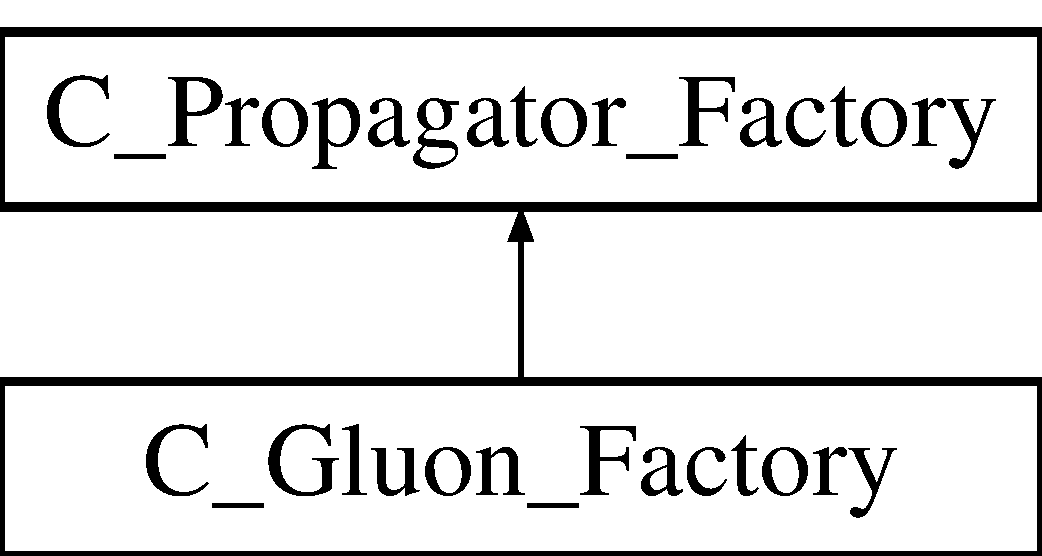
\includegraphics[height=2.000000cm]{class_c___gluon___factory}
\end{center}
\end{figure}
\subsection*{Public Member Functions}
\begin{DoxyCompactItemize}
\item 
\hypertarget{class_c___gluon___factory_a8c8da0ec99675366570f0ff44e390897}{\hyperlink{class_c___propagator}{C\-\_\-\-Propagator} $\ast$ {\bfseries Create} (int \-\_\-id)}\label{class_c___gluon___factory_a8c8da0ec99675366570f0ff44e390897}

\item 
\hypertarget{class_c___gluon___factory_a01429e9cb263d5c94b06cefae6b6cf5f}{\hyperlink{class_c___propagator}{C\-\_\-\-Propagator} $\ast$ {\bfseries Create} (int \-\_\-id, std\-::string \&\-\_\-\-Interpolation\-Points\-Path)}\label{class_c___gluon___factory_a01429e9cb263d5c94b06cefae6b6cf5f}

\end{DoxyCompactItemize}


The documentation for this class was generated from the following file\-:\begin{DoxyCompactItemize}
\item 
source/\-D\-S\-E/Propagator\-Factory.\-hpp\end{DoxyCompactItemize}

\hypertarget{class_c___integration___mockup}{\section{C\-\_\-\-Integration\-\_\-\-Mockup Class Reference}
\label{class_c___integration___mockup}\index{C\-\_\-\-Integration\-\_\-\-Mockup@{C\-\_\-\-Integration\-\_\-\-Mockup}}
}
\subsection*{Public Member Functions}
\begin{DoxyCompactItemize}
\item 
\hypertarget{class_c___integration___mockup_a277f0c63bed990b9c8beae175be845e6}{void {\bfseries set\-Function\-Type} (int \-\_\-\-\_\-int\-Function\-Type)}\label{class_c___integration___mockup_a277f0c63bed990b9c8beae175be845e6}

\item 
\hypertarget{class_c___integration___mockup_a0cf4106561a8032a45ab56d346ca48ed}{t\-\_\-d\-Matrix {\bfseries Integrand\-Mockup} (double x)}\label{class_c___integration___mockup_a0cf4106561a8032a45ab56d346ca48ed}

\item 
\hypertarget{class_c___integration___mockup_ae5fea8d5929f9e08bd8a520bc6fc007e}{double {\bfseries Function\-Line} (double x)}\label{class_c___integration___mockup_ae5fea8d5929f9e08bd8a520bc6fc007e}

\item 
\hypertarget{class_c___integration___mockup_abe3f2f04b984ae16533e71fa75a3ac43}{double {\bfseries Function\-Sine3x} (double x)}\label{class_c___integration___mockup_abe3f2f04b984ae16533e71fa75a3ac43}

\item 
\hypertarget{class_c___integration___mockup_a283bf7e4fa7926c5c309b3d05250857e}{double {\bfseries Function\-Cheb} (double x)}\label{class_c___integration___mockup_a283bf7e4fa7926c5c309b3d05250857e}

\item 
\hypertarget{class_c___integration___mockup_a6072270abf1e552a30b3b8eeaae56b57}{double {\bfseries Function\-Power} (double x)}\label{class_c___integration___mockup_a6072270abf1e552a30b3b8eeaae56b57}

\item 
\hypertarget{class_c___integration___mockup_ad0b2dc2666f3f535bb8de192dea15000}{double {\bfseries Function\-Cheb\-Cheb} (double x)}\label{class_c___integration___mockup_ad0b2dc2666f3f535bb8de192dea15000}

\item 
\hypertarget{class_c___integration___mockup_a98ac3a8fa83fd6696e34061aecd94e9c}{double {\bfseries Function\-Power\-Cheb} (double x)}\label{class_c___integration___mockup_a98ac3a8fa83fd6696e34061aecd94e9c}

\item 
\hypertarget{class_c___integration___mockup_ac29856604fcf4791fd4dd459ab8dd020}{int {\bfseries get\-Num\-Integration\-Points} ()}\label{class_c___integration___mockup_ac29856604fcf4791fd4dd459ab8dd020}

\item 
\hypertarget{class_c___integration___mockup_a2c945ead423a0e422a0e5d81dd6056fe}{double {\bfseries get\-Down\-Limit} ()}\label{class_c___integration___mockup_a2c945ead423a0e422a0e5d81dd6056fe}

\item 
\hypertarget{class_c___integration___mockup_ae46f0b9c1ab11f106b54c54c200583b9}{double {\bfseries get\-Up\-Limit} ()}\label{class_c___integration___mockup_ae46f0b9c1ab11f106b54c54c200583b9}

\end{DoxyCompactItemize}


The documentation for this class was generated from the following file\-:\begin{DoxyCompactItemize}
\item 
source/\-Mockups/Integration\-Mockups.\-hpp\end{DoxyCompactItemize}

\hypertarget{class_c___integration_nodes}{\section{C\-\_\-\-Integration\-Nodes Class Reference}
\label{class_c___integration_nodes}\index{C\-\_\-\-Integration\-Nodes@{C\-\_\-\-Integration\-Nodes}}
}


{\ttfamily \#include $<$Integration\-Nodes.\-hpp$>$}

Inheritance diagram for C\-\_\-\-Integration\-Nodes\-:\begin{figure}[H]
\begin{center}
\leavevmode
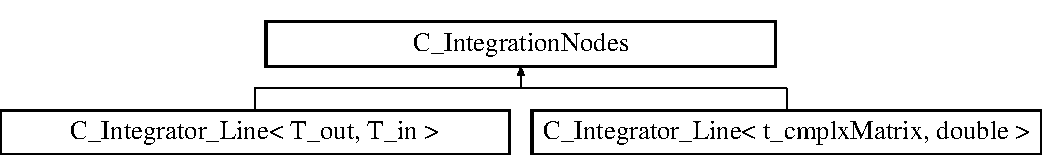
\includegraphics[height=2.000000cm]{class_c___integration_nodes}
\end{center}
\end{figure}
\subsection*{Public Member Functions}
\begin{DoxyCompactItemize}
\item 
void \hyperlink{class_c___integration_nodes_ad63bb8d4226180ecf6332852a52b702b}{get\-Nodes} (\hyperlink{types_8h_a7572e8a35cd6501ce959f177307310a4}{t\-\_\-d\-Array1\-D} \&\-\_\-x, \hyperlink{types_8h_a7572e8a35cd6501ce959f177307310a4}{t\-\_\-d\-Array1\-D} \&\-\_\-w)
\end{DoxyCompactItemize}
\subsection*{Protected Member Functions}
\begin{DoxyCompactItemize}
\item 
\hyperlink{class_c___integration_nodes_aae608186412f531e84601f7681d9a5ba}{C\-\_\-\-Integration\-Nodes} (int \-\_\-\-Num\-Points, double \-\_\-\-Lim\-Down, double \-\_\-\-Lim\-Up, int \-\_\-\-Num\-Aps, \hyperlink{_integration_nodes_8hpp_a8a2a136fba71c4785a5bdfe3e0e23b2b}{Integrator\-\_\-\-I\-D} \-\_\-id)
\item 
virtual \hyperlink{class_c___integration_nodes_aaba1eab67b07ff7ce5c16667aa9acda3}{$\sim$\-C\-\_\-\-Integration\-Nodes} ()
\item 
void \hyperlink{class_c___integration_nodes_a85fe5a11c29a8c59a75d5497901ca322}{gauleg} (double x1, double x2, \hyperlink{types_8h_a7572e8a35cd6501ce959f177307310a4}{t\-\_\-d\-Array1\-D} \&\hyperlink{class_c___integration_nodes_ac7482a184d19e0ec9bf62a99edd9e29b}{x}, \hyperlink{types_8h_a7572e8a35cd6501ce959f177307310a4}{t\-\_\-d\-Array1\-D} \&\hyperlink{class_c___integration_nodes_a023a6f295be0574aca58f8a67ac6263d}{w}, int n)
\item 
void \hyperlink{class_c___integration_nodes_a551c1c98b67b3def0e59e65e3d515401}{gaucheb} (double x1, double x2, \hyperlink{types_8h_a7572e8a35cd6501ce959f177307310a4}{t\-\_\-d\-Array1\-D} \&\hyperlink{class_c___integration_nodes_ac7482a184d19e0ec9bf62a99edd9e29b}{x}, \hyperlink{types_8h_a7572e8a35cd6501ce959f177307310a4}{t\-\_\-d\-Array1\-D} \&\hyperlink{class_c___integration_nodes_a023a6f295be0574aca58f8a67ac6263d}{w}, int n)
\item 
void \hyperlink{class_c___integration_nodes_ac368475cac1e355e8a4ee4e3354888ae}{set\-Nodes} (\hyperlink{_integration_nodes_8hpp_a8a2a136fba71c4785a5bdfe3e0e23b2b}{Integrator\-\_\-\-I\-D} \-\_\-id)
\end{DoxyCompactItemize}
\subsection*{Protected Attributes}
\begin{DoxyCompactItemize}
\item 
const double \hyperlink{class_c___integration_nodes_a2db6e5b500d59df584a1556fd2e928f4}{pi} =3.\-14159265358979
\item 
double \hyperlink{class_c___integration_nodes_a9d7f3f12030b61afb7d11ff833b92ab2}{Lim\-Up}
\item 
double \hyperlink{class_c___integration_nodes_aa2b7209a4f2aa65d90ca2cc1f22655ab}{Lim\-Down}
\item 
int \hyperlink{class_c___integration_nodes_a2aae6c2f677378b02fe1dd72137d5649}{Num\-Points}
\item 
int \hyperlink{class_c___integration_nodes_a1bf574f9151846abaeb89c2a9acca173}{Num\-Aps}
\item 
\hyperlink{types_8h_a7572e8a35cd6501ce959f177307310a4}{t\-\_\-d\-Array1\-D} \hyperlink{class_c___integration_nodes_abced67ac9650b49ca756fe34b0aa593a}{zz}
\item 
\hyperlink{types_8h_a7572e8a35cd6501ce959f177307310a4}{t\-\_\-d\-Array1\-D} \hyperlink{class_c___integration_nodes_a023a6f295be0574aca58f8a67ac6263d}{w}
\item 
\hyperlink{types_8h_a7572e8a35cd6501ce959f177307310a4}{t\-\_\-d\-Array1\-D} \hyperlink{class_c___integration_nodes_ac7482a184d19e0ec9bf62a99edd9e29b}{x}
\item 
\hyperlink{_integration_nodes_8hpp_a8a2a136fba71c4785a5bdfe3e0e23b2b}{Integrator\-\_\-\-I\-D} \hyperlink{class_c___integration_nodes_a1c7d0366d7ce1134f6a4c0944f80803b}{id}
\end{DoxyCompactItemize}


\subsection{Constructor \& Destructor Documentation}
\hypertarget{class_c___integration_nodes_aae608186412f531e84601f7681d9a5ba}{\index{C\-\_\-\-Integration\-Nodes@{C\-\_\-\-Integration\-Nodes}!C\-\_\-\-Integration\-Nodes@{C\-\_\-\-Integration\-Nodes}}
\index{C\-\_\-\-Integration\-Nodes@{C\-\_\-\-Integration\-Nodes}!C_IntegrationNodes@{C\-\_\-\-Integration\-Nodes}}
\subsubsection[{C\-\_\-\-Integration\-Nodes}]{\setlength{\rightskip}{0pt plus 5cm}C\-\_\-\-Integration\-Nodes\-::\-C\-\_\-\-Integration\-Nodes (
\begin{DoxyParamCaption}
\item[{int}]{\-\_\-\-Num\-Points, }
\item[{double}]{\-\_\-\-Lim\-Down, }
\item[{double}]{\-\_\-\-Lim\-Up, }
\item[{int}]{\-\_\-\-Num\-Aps, }
\item[{{\bf Integrator\-\_\-\-I\-D}}]{\-\_\-id}
\end{DoxyParamCaption}
)\hspace{0.3cm}{\ttfamily [inline]}, {\ttfamily [protected]}}}\label{class_c___integration_nodes_aae608186412f531e84601f7681d9a5ba}
\hypertarget{class_c___integration_nodes_aaba1eab67b07ff7ce5c16667aa9acda3}{\index{C\-\_\-\-Integration\-Nodes@{C\-\_\-\-Integration\-Nodes}!$\sim$\-C\-\_\-\-Integration\-Nodes@{$\sim$\-C\-\_\-\-Integration\-Nodes}}
\index{$\sim$\-C\-\_\-\-Integration\-Nodes@{$\sim$\-C\-\_\-\-Integration\-Nodes}!C_IntegrationNodes@{C\-\_\-\-Integration\-Nodes}}
\subsubsection[{$\sim$\-C\-\_\-\-Integration\-Nodes}]{\setlength{\rightskip}{0pt plus 5cm}virtual C\-\_\-\-Integration\-Nodes\-::$\sim$\-C\-\_\-\-Integration\-Nodes (
\begin{DoxyParamCaption}
{}
\end{DoxyParamCaption}
)\hspace{0.3cm}{\ttfamily [inline]}, {\ttfamily [protected]}, {\ttfamily [virtual]}}}\label{class_c___integration_nodes_aaba1eab67b07ff7ce5c16667aa9acda3}


\subsection{Member Function Documentation}
\hypertarget{class_c___integration_nodes_a551c1c98b67b3def0e59e65e3d515401}{\index{C\-\_\-\-Integration\-Nodes@{C\-\_\-\-Integration\-Nodes}!gaucheb@{gaucheb}}
\index{gaucheb@{gaucheb}!C_IntegrationNodes@{C\-\_\-\-Integration\-Nodes}}
\subsubsection[{gaucheb}]{\setlength{\rightskip}{0pt plus 5cm}void C\-\_\-\-Integration\-Nodes\-::gaucheb (
\begin{DoxyParamCaption}
\item[{double}]{x1, }
\item[{double}]{x2, }
\item[{{\bf t\-\_\-d\-Array1\-D} \&}]{x, }
\item[{{\bf t\-\_\-d\-Array1\-D} \&}]{w, }
\item[{int}]{n}
\end{DoxyParamCaption}
)\hspace{0.3cm}{\ttfamily [inline]}, {\ttfamily [protected]}}}\label{class_c___integration_nodes_a551c1c98b67b3def0e59e65e3d515401}
\hypertarget{class_c___integration_nodes_a85fe5a11c29a8c59a75d5497901ca322}{\index{C\-\_\-\-Integration\-Nodes@{C\-\_\-\-Integration\-Nodes}!gauleg@{gauleg}}
\index{gauleg@{gauleg}!C_IntegrationNodes@{C\-\_\-\-Integration\-Nodes}}
\subsubsection[{gauleg}]{\setlength{\rightskip}{0pt plus 5cm}void C\-\_\-\-Integration\-Nodes\-::gauleg (
\begin{DoxyParamCaption}
\item[{double}]{x1, }
\item[{double}]{x2, }
\item[{{\bf t\-\_\-d\-Array1\-D} \&}]{x, }
\item[{{\bf t\-\_\-d\-Array1\-D} \&}]{w, }
\item[{int}]{n}
\end{DoxyParamCaption}
)\hspace{0.3cm}{\ttfamily [inline]}, {\ttfamily [protected]}}}\label{class_c___integration_nodes_a85fe5a11c29a8c59a75d5497901ca322}
\hypertarget{class_c___integration_nodes_ad63bb8d4226180ecf6332852a52b702b}{\index{C\-\_\-\-Integration\-Nodes@{C\-\_\-\-Integration\-Nodes}!get\-Nodes@{get\-Nodes}}
\index{get\-Nodes@{get\-Nodes}!C_IntegrationNodes@{C\-\_\-\-Integration\-Nodes}}
\subsubsection[{get\-Nodes}]{\setlength{\rightskip}{0pt plus 5cm}void C\-\_\-\-Integration\-Nodes\-::get\-Nodes (
\begin{DoxyParamCaption}
\item[{{\bf t\-\_\-d\-Array1\-D} \&}]{\-\_\-x, }
\item[{{\bf t\-\_\-d\-Array1\-D} \&}]{\-\_\-w}
\end{DoxyParamCaption}
)\hspace{0.3cm}{\ttfamily [inline]}}}\label{class_c___integration_nodes_ad63bb8d4226180ecf6332852a52b702b}
\hypertarget{class_c___integration_nodes_ac368475cac1e355e8a4ee4e3354888ae}{\index{C\-\_\-\-Integration\-Nodes@{C\-\_\-\-Integration\-Nodes}!set\-Nodes@{set\-Nodes}}
\index{set\-Nodes@{set\-Nodes}!C_IntegrationNodes@{C\-\_\-\-Integration\-Nodes}}
\subsubsection[{set\-Nodes}]{\setlength{\rightskip}{0pt plus 5cm}void C\-\_\-\-Integration\-Nodes\-::set\-Nodes (
\begin{DoxyParamCaption}
\item[{{\bf Integrator\-\_\-\-I\-D}}]{\-\_\-id}
\end{DoxyParamCaption}
)\hspace{0.3cm}{\ttfamily [inline]}, {\ttfamily [protected]}}}\label{class_c___integration_nodes_ac368475cac1e355e8a4ee4e3354888ae}


\subsection{Member Data Documentation}
\hypertarget{class_c___integration_nodes_a1c7d0366d7ce1134f6a4c0944f80803b}{\index{C\-\_\-\-Integration\-Nodes@{C\-\_\-\-Integration\-Nodes}!id@{id}}
\index{id@{id}!C_IntegrationNodes@{C\-\_\-\-Integration\-Nodes}}
\subsubsection[{id}]{\setlength{\rightskip}{0pt plus 5cm}{\bf Integrator\-\_\-\-I\-D} C\-\_\-\-Integration\-Nodes\-::id\hspace{0.3cm}{\ttfamily [protected]}}}\label{class_c___integration_nodes_a1c7d0366d7ce1134f6a4c0944f80803b}
\hypertarget{class_c___integration_nodes_aa2b7209a4f2aa65d90ca2cc1f22655ab}{\index{C\-\_\-\-Integration\-Nodes@{C\-\_\-\-Integration\-Nodes}!Lim\-Down@{Lim\-Down}}
\index{Lim\-Down@{Lim\-Down}!C_IntegrationNodes@{C\-\_\-\-Integration\-Nodes}}
\subsubsection[{Lim\-Down}]{\setlength{\rightskip}{0pt plus 5cm}double C\-\_\-\-Integration\-Nodes\-::\-Lim\-Down\hspace{0.3cm}{\ttfamily [protected]}}}\label{class_c___integration_nodes_aa2b7209a4f2aa65d90ca2cc1f22655ab}
\hypertarget{class_c___integration_nodes_a9d7f3f12030b61afb7d11ff833b92ab2}{\index{C\-\_\-\-Integration\-Nodes@{C\-\_\-\-Integration\-Nodes}!Lim\-Up@{Lim\-Up}}
\index{Lim\-Up@{Lim\-Up}!C_IntegrationNodes@{C\-\_\-\-Integration\-Nodes}}
\subsubsection[{Lim\-Up}]{\setlength{\rightskip}{0pt plus 5cm}double C\-\_\-\-Integration\-Nodes\-::\-Lim\-Up\hspace{0.3cm}{\ttfamily [protected]}}}\label{class_c___integration_nodes_a9d7f3f12030b61afb7d11ff833b92ab2}
\hypertarget{class_c___integration_nodes_a1bf574f9151846abaeb89c2a9acca173}{\index{C\-\_\-\-Integration\-Nodes@{C\-\_\-\-Integration\-Nodes}!Num\-Aps@{Num\-Aps}}
\index{Num\-Aps@{Num\-Aps}!C_IntegrationNodes@{C\-\_\-\-Integration\-Nodes}}
\subsubsection[{Num\-Aps}]{\setlength{\rightskip}{0pt plus 5cm}int C\-\_\-\-Integration\-Nodes\-::\-Num\-Aps\hspace{0.3cm}{\ttfamily [protected]}}}\label{class_c___integration_nodes_a1bf574f9151846abaeb89c2a9acca173}
\hypertarget{class_c___integration_nodes_a2aae6c2f677378b02fe1dd72137d5649}{\index{C\-\_\-\-Integration\-Nodes@{C\-\_\-\-Integration\-Nodes}!Num\-Points@{Num\-Points}}
\index{Num\-Points@{Num\-Points}!C_IntegrationNodes@{C\-\_\-\-Integration\-Nodes}}
\subsubsection[{Num\-Points}]{\setlength{\rightskip}{0pt plus 5cm}int C\-\_\-\-Integration\-Nodes\-::\-Num\-Points\hspace{0.3cm}{\ttfamily [protected]}}}\label{class_c___integration_nodes_a2aae6c2f677378b02fe1dd72137d5649}
\hypertarget{class_c___integration_nodes_a2db6e5b500d59df584a1556fd2e928f4}{\index{C\-\_\-\-Integration\-Nodes@{C\-\_\-\-Integration\-Nodes}!pi@{pi}}
\index{pi@{pi}!C_IntegrationNodes@{C\-\_\-\-Integration\-Nodes}}
\subsubsection[{pi}]{\setlength{\rightskip}{0pt plus 5cm}const double C\-\_\-\-Integration\-Nodes\-::pi =3.\-14159265358979\hspace{0.3cm}{\ttfamily [protected]}}}\label{class_c___integration_nodes_a2db6e5b500d59df584a1556fd2e928f4}
\hypertarget{class_c___integration_nodes_a023a6f295be0574aca58f8a67ac6263d}{\index{C\-\_\-\-Integration\-Nodes@{C\-\_\-\-Integration\-Nodes}!w@{w}}
\index{w@{w}!C_IntegrationNodes@{C\-\_\-\-Integration\-Nodes}}
\subsubsection[{w}]{\setlength{\rightskip}{0pt plus 5cm}{\bf t\-\_\-d\-Array1\-D} C\-\_\-\-Integration\-Nodes\-::w\hspace{0.3cm}{\ttfamily [protected]}}}\label{class_c___integration_nodes_a023a6f295be0574aca58f8a67ac6263d}
\hypertarget{class_c___integration_nodes_ac7482a184d19e0ec9bf62a99edd9e29b}{\index{C\-\_\-\-Integration\-Nodes@{C\-\_\-\-Integration\-Nodes}!x@{x}}
\index{x@{x}!C_IntegrationNodes@{C\-\_\-\-Integration\-Nodes}}
\subsubsection[{x}]{\setlength{\rightskip}{0pt plus 5cm}{\bf t\-\_\-d\-Array1\-D} C\-\_\-\-Integration\-Nodes\-::x\hspace{0.3cm}{\ttfamily [protected]}}}\label{class_c___integration_nodes_ac7482a184d19e0ec9bf62a99edd9e29b}
\hypertarget{class_c___integration_nodes_abced67ac9650b49ca756fe34b0aa593a}{\index{C\-\_\-\-Integration\-Nodes@{C\-\_\-\-Integration\-Nodes}!zz@{zz}}
\index{zz@{zz}!C_IntegrationNodes@{C\-\_\-\-Integration\-Nodes}}
\subsubsection[{zz}]{\setlength{\rightskip}{0pt plus 5cm}{\bf t\-\_\-d\-Array1\-D} C\-\_\-\-Integration\-Nodes\-::zz\hspace{0.3cm}{\ttfamily [protected]}}}\label{class_c___integration_nodes_abced67ac9650b49ca756fe34b0aa593a}


The documentation for this class was generated from the following file\-:\begin{DoxyCompactItemize}
\item 
source/\-Num\-Libs/\hyperlink{_integration_nodes_8hpp}{Integration\-Nodes.\-hpp}\end{DoxyCompactItemize}

\hypertarget{class_c___integrator___line}{\section{C\-\_\-\-Integrator\-\_\-\-Line$<$ T\-\_\-out, T\-\_\-in $>$ Class Template Reference}
\label{class_c___integrator___line}\index{C\-\_\-\-Integrator\-\_\-\-Line$<$ T\-\_\-out, T\-\_\-in $>$@{C\-\_\-\-Integrator\-\_\-\-Line$<$ T\-\_\-out, T\-\_\-in $>$}}
}
Inheritance diagram for C\-\_\-\-Integrator\-\_\-\-Line$<$ T\-\_\-out, T\-\_\-in $>$\-:\begin{figure}[H]
\begin{center}
\leavevmode
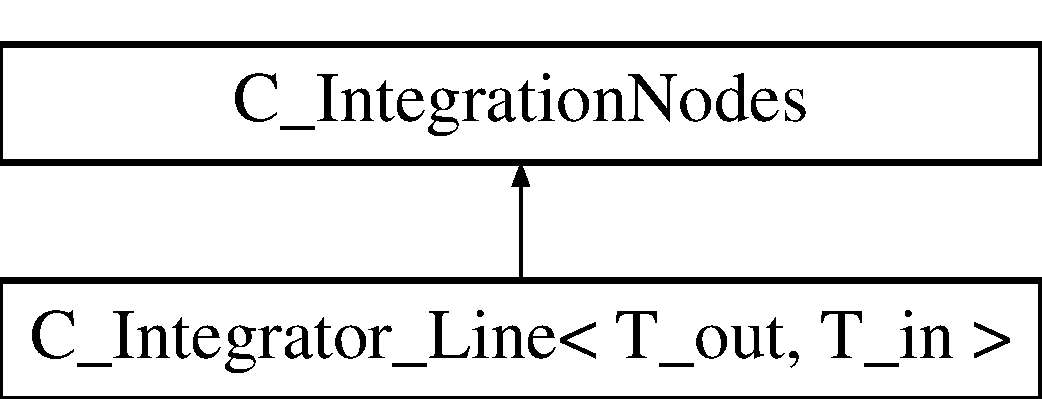
\includegraphics[height=2.000000cm]{class_c___integrator___line}
\end{center}
\end{figure}
\subsection*{Public Member Functions}
\begin{DoxyCompactItemize}
\item 
\hypertarget{class_c___integrator___line_a36990ef563e884b91912f8050ab85fff}{T\-\_\-out {\bfseries get\-Result} (std\-::function$<$ T\-\_\-out(T\-\_\-in)$>$ $\ast$Integrand)}\label{class_c___integrator___line_a36990ef563e884b91912f8050ab85fff}

\end{DoxyCompactItemize}
\subsection*{Static Public Member Functions}
\begin{DoxyCompactItemize}
\item 
\hypertarget{class_c___integrator___line_a39a1ca043cff260ffe3fa4e7bc61c5e7}{static \hyperlink{class_c___integrator___line}{C\-\_\-\-Integrator\-\_\-\-Line} $\ast$ {\bfseries create\-Integrator} (int \-\_\-\-Num\-Points, double \-\_\-\-Lim\-Down, double \-\_\-\-Lim\-Up, int \-\_\-\-Num\-Aps, Integrator\-\_\-\-I\-D \-\_\-id)}\label{class_c___integrator___line_a39a1ca043cff260ffe3fa4e7bc61c5e7}

\end{DoxyCompactItemize}
\subsection*{Protected Member Functions}
\begin{DoxyCompactItemize}
\item 
\hypertarget{class_c___integrator___line_a296717ff620c356cbe2b16b3cca73d16}{{\bfseries C\-\_\-\-Integrator\-\_\-\-Line} (int \-\_\-\-Num\-Points, double \-\_\-\-Lim\-Down, double \-\_\-\-Lim\-Up, int \-\_\-\-Num\-Aps, Integrator\-\_\-\-I\-D \-\_\-id)}\label{class_c___integrator___line_a296717ff620c356cbe2b16b3cca73d16}

\end{DoxyCompactItemize}
\subsection*{Protected Attributes}
\begin{DoxyCompactItemize}
\item 
\hypertarget{class_c___integrator___line_a9cd6c7764ef843fc38521254ebdc3ada}{std\-::function$<$ T\-\_\-out(T\-\_\-in)$>$ $\ast$ {\bfseries Integrand}}\label{class_c___integrator___line_a9cd6c7764ef843fc38521254ebdc3ada}

\end{DoxyCompactItemize}


The documentation for this class was generated from the following file\-:\begin{DoxyCompactItemize}
\item 
source/\-Num\-Libs/Integrator.\-hpp\end{DoxyCompactItemize}

\hypertarget{class_c___integrator___path}{\section{C\-\_\-\-Integrator\-\_\-\-Path$<$ T\-\_\-out, T\-\_\-contour, T\-\_\-in $>$ Class Template Reference}
\label{class_c___integrator___path}\index{C\-\_\-\-Integrator\-\_\-\-Path$<$ T\-\_\-out, T\-\_\-contour, T\-\_\-in $>$@{C\-\_\-\-Integrator\-\_\-\-Path$<$ T\-\_\-out, T\-\_\-contour, T\-\_\-in $>$}}
}
\subsection*{Public Member Functions}
\begin{DoxyCompactItemize}
\item 
\hypertarget{class_c___integrator___path_a95026f1b45d90861f246b828ce9131c0}{vector$<$ T\-\_\-out $>$ {\bfseries get\-Result} (T\-\_\-contour \&Path\-Storage, T\-\_\-in \&Point)}\label{class_c___integrator___path_a95026f1b45d90861f246b828ce9131c0}

\end{DoxyCompactItemize}
\subsection*{Static Public Member Functions}
\begin{DoxyCompactItemize}
\item 
\hypertarget{class_c___integrator___path_ad68512fccb5e8ef0402b214401268a2a}{static \hyperlink{class_c___integrator___path}{C\-\_\-\-Integrator\-\_\-\-Path} $\ast$ {\bfseries create\-Integrator} (int \-\_\-\-Num\-Points, std\-::function$<$ T\-\_\-in(T\-\_\-in, T\-\_\-in)$>$ $\ast$\-\_\-\-Integration\-Weight\-Function)}\label{class_c___integrator___path_ad68512fccb5e8ef0402b214401268a2a}

\end{DoxyCompactItemize}
\subsection*{Protected Member Functions}
\begin{DoxyCompactItemize}
\item 
\hypertarget{class_c___integrator___path_ab4acfaa64baff2436a466a3e2f099827}{{\bfseries C\-\_\-\-Integrator\-\_\-\-Path} (int \-\_\-\-Num\-Aps)}\label{class_c___integrator___path_ab4acfaa64baff2436a466a3e2f099827}

\item 
\hypertarget{class_c___integrator___path_ab02353508a8140cafd2d2cf1ad8368ac}{void {\bfseries set\-Integration\-Weight\-Function} (std\-::function$<$ T\-\_\-in(T\-\_\-in, T\-\_\-in)$>$ $\ast$\-\_\-\-Integration\-Weight\-Function)}\label{class_c___integrator___path_ab02353508a8140cafd2d2cf1ad8368ac}

\end{DoxyCompactItemize}
\subsection*{Protected Attributes}
\begin{DoxyCompactItemize}
\item 
\hypertarget{class_c___integrator___path_ae229090f61dadfaec6eb74eea341de53}{int {\bfseries Num\-Amps}}\label{class_c___integrator___path_ae229090f61dadfaec6eb74eea341de53}

\item 
\hypertarget{class_c___integrator___path_aefd642a90c8bd5064c1c39c96e58756d}{std\-::function$<$ T\-\_\-in(T\-\_\-in, T\-\_\-in)$>$ $\ast$ {\bfseries Integration\-Weight\-Function}}\label{class_c___integrator___path_aefd642a90c8bd5064c1c39c96e58756d}

\end{DoxyCompactItemize}


The documentation for this class was generated from the following file\-:\begin{DoxyCompactItemize}
\item 
source/\-Num\-Libs/Integrator\-\_\-\-Path.\-hpp\end{DoxyCompactItemize}

\hypertarget{class_c___kernel___factory}{\section{C\-\_\-\-Kernel\-\_\-\-Factory Class Reference}
\label{class_c___kernel___factory}\index{C\-\_\-\-Kernel\-\_\-\-Factory@{C\-\_\-\-Kernel\-\_\-\-Factory}}
}


{\ttfamily \#include $<$Kernel\-Factory.\-hpp$>$}

\subsection*{Public Member Functions}
\begin{DoxyCompactItemize}
\item 
\hyperlink{class_c___abstract_kernel}{C\-\_\-\-Abstract\-Kernel} $\ast$ \hyperlink{class_c___kernel___factory_a4e0263fb3805d2abf65c45d12ac2365e}{Create} (\hyperlink{_abstract_kernel_8hpp_acee766998fbe394072b4d2fe1eb50e62}{Kernel\-\_\-\-I\-D} \-\_\-id)
\end{DoxyCompactItemize}
\subsection*{Static Public Member Functions}
\begin{DoxyCompactItemize}
\item 
static \hyperlink{class_c___kernel___factory}{C\-\_\-\-Kernel\-\_\-\-Factory} \& \hyperlink{class_c___kernel___factory_aec66c34d2fb1224aadda12ea4865e281}{instance} ()
\end{DoxyCompactItemize}


\subsection{Member Function Documentation}
\hypertarget{class_c___kernel___factory_a4e0263fb3805d2abf65c45d12ac2365e}{\index{C\-\_\-\-Kernel\-\_\-\-Factory@{C\-\_\-\-Kernel\-\_\-\-Factory}!Create@{Create}}
\index{Create@{Create}!C_Kernel_Factory@{C\-\_\-\-Kernel\-\_\-\-Factory}}
\subsubsection[{Create}]{\setlength{\rightskip}{0pt plus 5cm}{\bf C\-\_\-\-Abstract\-Kernel}$\ast$ C\-\_\-\-Kernel\-\_\-\-Factory\-::\-Create (
\begin{DoxyParamCaption}
\item[{{\bf Kernel\-\_\-\-I\-D}}]{\-\_\-id}
\end{DoxyParamCaption}
)\hspace{0.3cm}{\ttfamily [inline]}}}\label{class_c___kernel___factory_a4e0263fb3805d2abf65c45d12ac2365e}
\hypertarget{class_c___kernel___factory_aec66c34d2fb1224aadda12ea4865e281}{\index{C\-\_\-\-Kernel\-\_\-\-Factory@{C\-\_\-\-Kernel\-\_\-\-Factory}!instance@{instance}}
\index{instance@{instance}!C_Kernel_Factory@{C\-\_\-\-Kernel\-\_\-\-Factory}}
\subsubsection[{instance}]{\setlength{\rightskip}{0pt plus 5cm}static {\bf C\-\_\-\-Kernel\-\_\-\-Factory}\& C\-\_\-\-Kernel\-\_\-\-Factory\-::instance (
\begin{DoxyParamCaption}
{}
\end{DoxyParamCaption}
)\hspace{0.3cm}{\ttfamily [inline]}, {\ttfamily [static]}}}\label{class_c___kernel___factory_aec66c34d2fb1224aadda12ea4865e281}


The documentation for this class was generated from the following file\-:\begin{DoxyCompactItemize}
\item 
source/\-Kernel/\hyperlink{_kernel_factory_8hpp}{Kernel\-Factory.\-hpp}\end{DoxyCompactItemize}

\hypertarget{class_c___kernel___r_l}{\section{C\-\_\-\-Kernel\-\_\-\-R\-L Class Reference}
\label{class_c___kernel___r_l}\index{C\-\_\-\-Kernel\-\_\-\-R\-L@{C\-\_\-\-Kernel\-\_\-\-R\-L}}
}
Inheritance diagram for C\-\_\-\-Kernel\-\_\-\-R\-L\-:\begin{figure}[H]
\begin{center}
\leavevmode
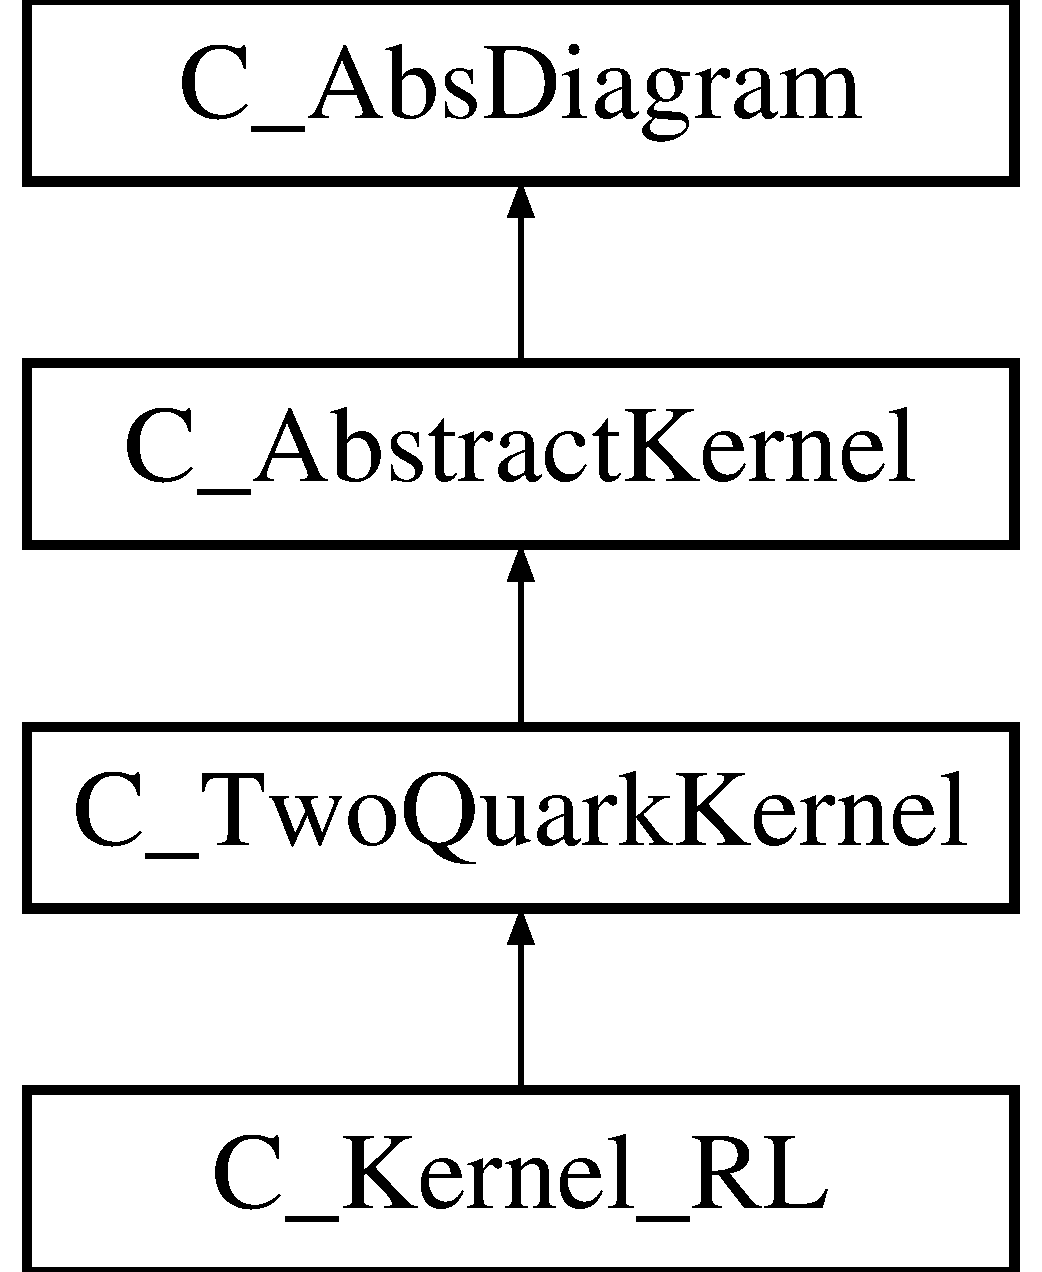
\includegraphics[height=3.000000cm]{class_c___kernel___r_l}
\end{center}
\end{figure}
\subsection*{Public Member Functions}
\begin{DoxyCompactItemize}
\item 
\hypertarget{class_c___kernel___r_l_a456dc18a4f961f9f3d8d1a51917eee8c}{void {\bfseries info} ()}\label{class_c___kernel___r_l_a456dc18a4f961f9f3d8d1a51917eee8c}

\item 
\hypertarget{class_c___kernel___r_l_abb7217ca0b629a6d28f460f27b0b3306}{void {\bfseries set\-Mediators} (t\-\_\-cmplx\-Vector \&k, t\-\_\-cmplx\-Vector \&p, t\-\_\-cmplx\-Vector \&P, std\-::vector$<$ t\-\_\-cmplx\-Tensor $>$ \&Mediators)}\label{class_c___kernel___r_l_abb7217ca0b629a6d28f460f27b0b3306}

\item 
\hypertarget{class_c___kernel___r_l_a74a876dbb773d242c6264182c7949ca2}{t\-\_\-cmplx {\bfseries Element\-Kmatrix} (int t, int s, int r, int u, std\-::vector$<$ t\-\_\-cmplx\-Tensor $>$ \&Mediators)}\label{class_c___kernel___r_l_a74a876dbb773d242c6264182c7949ca2}

\end{DoxyCompactItemize}
\subsection*{Public Attributes}
\begin{DoxyCompactItemize}
\item 
\hypertarget{class_c___kernel___r_l_aac0de569f84bb52bb886fc8e619311f5}{t\-\_\-cmplx {\bfseries Z2}}\label{class_c___kernel___r_l_aac0de569f84bb52bb886fc8e619311f5}

\end{DoxyCompactItemize}
\subsection*{Additional Inherited Members}


The documentation for this class was generated from the following files\-:\begin{DoxyCompactItemize}
\item 
source/\-Kernel/Rainbow\-Ladder\-Kernel.\-hpp\item 
source/\-Kernel/Rainbow\-Ladder\-Kernel.\-cpp\end{DoxyCompactItemize}

\hypertarget{class_c___kernel___r_l___p_s}{\section{C\-\_\-\-Kernel\-\_\-\-R\-L\-\_\-\-P\-S Class Reference}
\label{class_c___kernel___r_l___p_s}\index{C\-\_\-\-Kernel\-\_\-\-R\-L\-\_\-\-P\-S@{C\-\_\-\-Kernel\-\_\-\-R\-L\-\_\-\-P\-S}}
}
Inheritance diagram for C\-\_\-\-Kernel\-\_\-\-R\-L\-\_\-\-P\-S\-:\begin{figure}[H]
\begin{center}
\leavevmode
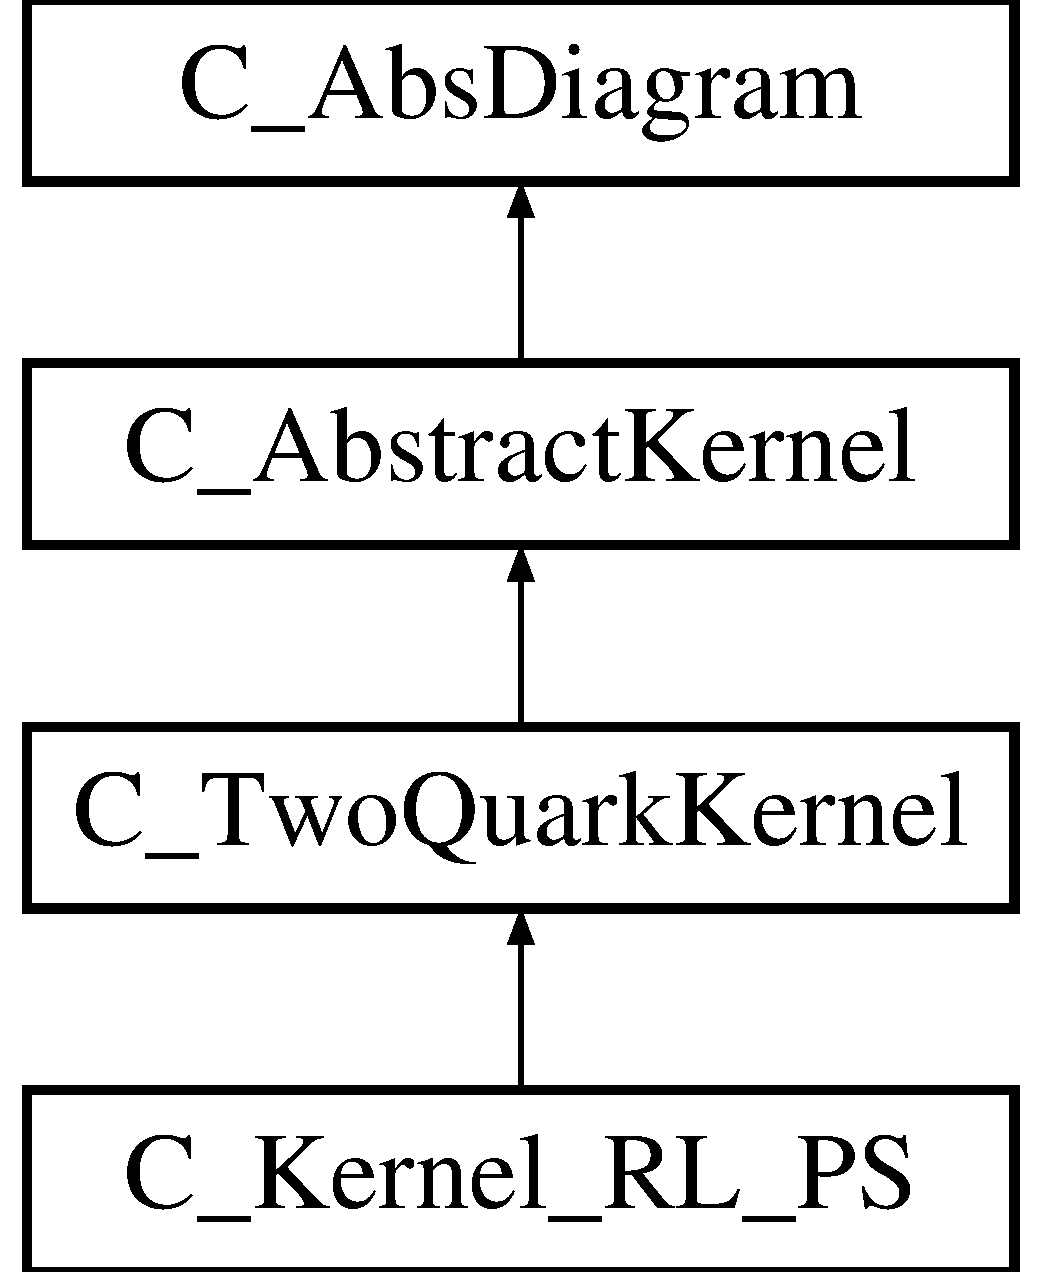
\includegraphics[height=3.000000cm]{class_c___kernel___r_l___p_s}
\end{center}
\end{figure}
\subsection*{Public Member Functions}
\begin{DoxyCompactItemize}
\item 
\hypertarget{class_c___kernel___r_l___p_s_ab0bfc75c8acd42ade61f354e6203c74d}{void {\bfseries info} ()}\label{class_c___kernel___r_l___p_s_ab0bfc75c8acd42ade61f354e6203c74d}

\item 
\hypertarget{class_c___kernel___r_l___p_s_ad25fe96108843a814f55b5c619c5187e}{void {\bfseries set\-Meson\-Exchange\-Mass} (t\-\_\-cmplx \-\_\-\-M)}\label{class_c___kernel___r_l___p_s_ad25fe96108843a814f55b5c619c5187e}

\item 
\hypertarget{class_c___kernel___r_l___p_s_a5d635af404489de546e6240b8d2a9265}{void {\bfseries set\-Mediators} (t\-\_\-cmplx\-Vector \&k, t\-\_\-cmplx\-Vector \&p, t\-\_\-cmplx\-Vector \&P, std\-::vector$<$ t\-\_\-cmplx\-Tensor $>$ \&Mediators)}\label{class_c___kernel___r_l___p_s_a5d635af404489de546e6240b8d2a9265}

\item 
\hypertarget{class_c___kernel___r_l___p_s_a57c4a7e5c0c4db8d61a8b547ae9f23af}{t\-\_\-cmplx {\bfseries Element\-Kmatrix} (int t, int s, int r, int u, std\-::vector$<$ t\-\_\-cmplx\-Tensor $>$ \&Mediators)}\label{class_c___kernel___r_l___p_s_a57c4a7e5c0c4db8d61a8b547ae9f23af}

\item 
\hypertarget{class_c___kernel___r_l___p_s_a6323065c3d5d268f755a7107ffea5506}{t\-\_\-cmplx {\bfseries Vertex\-Dressing\-At} (int kernel\-\_\-type, int num\-\_\-\-P, int num\-\_\-amp, t\-\_\-cmplx coordin)}\label{class_c___kernel___r_l___p_s_a6323065c3d5d268f755a7107ffea5506}

\item 
\hypertarget{class_c___kernel___r_l___p_s_abbad3a288bd15c6d4ce71f2880f096cf}{t\-\_\-cmplx {\bfseries Set\-Interpolation} (t\-\_\-cmplx vertex\-\_\-momenta, t\-\_\-cmplx prop\-\_\-momenta)}\label{class_c___kernel___r_l___p_s_abbad3a288bd15c6d4ce71f2880f096cf}

\item 
\hypertarget{class_c___kernel___r_l___p_s_a59837c29b2f0f580bba3f506998b5095}{t\-\_\-cmplx\-Tensor {\bfseries Set\-P\-S\-Matrix\-\_\-etta\-\_\-quark} (t\-\_\-cmplx \&vertex\-\_\-momenta, t\-\_\-cmplx \&prop\-\_\-momenta)}\label{class_c___kernel___r_l___p_s_a59837c29b2f0f580bba3f506998b5095}

\item 
\hypertarget{class_c___kernel___r_l___p_s_a727f610ca37be4a8c379f0a32ca43301}{t\-\_\-cmplx\-Tensor {\bfseries Set\-P\-S\-Matrix\-\_\-etta\-\_\-\-B\-S\-E} (t\-\_\-cmplx \&vertex\-\_\-momenta, t\-\_\-cmplx \&prop\-\_\-momenta)}\label{class_c___kernel___r_l___p_s_a727f610ca37be4a8c379f0a32ca43301}

\item 
\hypertarget{class_c___kernel___r_l___p_s_aa9e8de0d2615d212c08522fb004d9e9a}{t\-\_\-cmplx\-Tensor {\bfseries Set\-P\-S\-Matrix\-\_\-pion\-\_\-quark} (t\-\_\-cmplx \&vertex\-\_\-momenta, t\-\_\-cmplx \&prop\-\_\-momenta)}\label{class_c___kernel___r_l___p_s_aa9e8de0d2615d212c08522fb004d9e9a}

\item 
\hypertarget{class_c___kernel___r_l___p_s_afe3f06a61a5fa9cd043e4c4319fec8b0}{t\-\_\-cmplx\-Tensor {\bfseries Set\-P\-S\-Matrix\-\_\-pion\-\_\-\-B\-S\-E} (t\-\_\-cmplx \&vertex\-\_\-momenta, t\-\_\-cmplx \&prop\-\_\-momenta)}\label{class_c___kernel___r_l___p_s_afe3f06a61a5fa9cd043e4c4319fec8b0}

\item 
\hypertarget{class_c___kernel___r_l___p_s_a80a925fa85452e40566f03a9ba8e0e06}{void {\bfseries set\-Convolution\-Type} (int type)}\label{class_c___kernel___r_l___p_s_a80a925fa85452e40566f03a9ba8e0e06}

\end{DoxyCompactItemize}
\subsection*{Protected Attributes}
\begin{DoxyCompactItemize}
\item 
\hypertarget{class_c___kernel___r_l___p_s_adf4728ca0caa741eb5242e4c8b67ef44}{t\-\_\-cmplx\-Tensor(C\-\_\-\-Kernel\-\_\-\-R\-L\-\_\-\-P\-S\-::$\ast$ {\bfseries Set\-P\-S\-Matrix} )(t\-\_\-cmplx \&, t\-\_\-cmplx \&)}\label{class_c___kernel___r_l___p_s_adf4728ca0caa741eb5242e4c8b67ef44}

\item 
\hypertarget{class_c___kernel___r_l___p_s_a737ca2c158cc24d99d183314cd4ef248}{t\-\_\-cmplx {\bfseries Z2}}\label{class_c___kernel___r_l___p_s_a737ca2c158cc24d99d183314cd4ef248}

\item 
\hypertarget{class_c___kernel___r_l___p_s_afa5aab2c72c55dd84fd3dd0f4a6e374b}{t\-\_\-cmplx {\bfseries Pseudo\-Meson\-Mass}}\label{class_c___kernel___r_l___p_s_afa5aab2c72c55dd84fd3dd0f4a6e374b}

\end{DoxyCompactItemize}
\subsection*{Additional Inherited Members}


The documentation for this class was generated from the following files\-:\begin{DoxyCompactItemize}
\item 
source/\-Kernel/R\-Land\-Pseudo\-Scalar.\-hpp\item 
source/\-Kernel/R\-Land\-Pseudo\-Scalar.\-cpp\end{DoxyCompactItemize}

\hypertarget{class_c___kinematics__1loop}{\section{C\-\_\-\-Kinematics\-\_\-1loop Class Reference}
\label{class_c___kinematics__1loop}\index{C\-\_\-\-Kinematics\-\_\-1loop@{C\-\_\-\-Kinematics\-\_\-1loop}}
}
\subsection*{Public Member Functions}
\begin{DoxyCompactItemize}
\item 
\hypertarget{class_c___kinematics__1loop_ac8ea5c0bc49a996a39f5d9bb9be77938}{void {\bfseries Set\-Vector\-\_\-\-P} (t\-\_\-cmplx P\-\_\-v)}\label{class_c___kinematics__1loop_ac8ea5c0bc49a996a39f5d9bb9be77938}

\item 
\hypertarget{class_c___kinematics__1loop_a19d01bd7b6d4823e432fe4b6e93bb5cb}{void {\bfseries Set\-Vector\-\_\-\-K} (t\-\_\-cmplx K\-\_\-v)}\label{class_c___kinematics__1loop_a19d01bd7b6d4823e432fe4b6e93bb5cb}

\item 
\hypertarget{class_c___kinematics__1loop_af2e051a57be7c9f8b4f82c9c8075f66f}{void {\bfseries Set\-Vectors\-\_\-p} (t\-\_\-cmplx z\-\_\-ex, t\-\_\-cmplx p\-\_\-ex)}\label{class_c___kinematics__1loop_af2e051a57be7c9f8b4f82c9c8075f66f}

\item 
\hypertarget{class_c___kinematics__1loop_a5f1fac5360637bd87b4cf4cf29577e41}{void {\bfseries Set\-Vectors\-\_\-k} (double \-\_\-zetta, t\-\_\-cmplx x, t\-\_\-cmplx y, t\-\_\-cmplx z)}\label{class_c___kinematics__1loop_a5f1fac5360637bd87b4cf4cf29577e41}

\item 
\hypertarget{class_c___kinematics__1loop_aa93f0b39da69100d1801a9d525b65fff}{void {\bfseries Set\-Vectors\-\_\-q} ()}\label{class_c___kinematics__1loop_aa93f0b39da69100d1801a9d525b65fff}

\item 
\hypertarget{class_c___kinematics__1loop_a9d78b3129c3eefedb197f1fd13c341e7}{void {\bfseries Set\-Vestors\-\_\-k\-\_\-for\-\_\-\-S} (double \-\_\-zetta, t\-\_\-cmplx\-Vector \-\_\-k)}\label{class_c___kinematics__1loop_a9d78b3129c3eefedb197f1fd13c341e7}

\item 
\hypertarget{class_c___kinematics__1loop_a9ea61128f7fc8f0c43ba3a7ca649059f}{t\-\_\-cmplx\-Dirac {\bfseries Trans\-In} (t\-\_\-cmplx\-Dirac \-\_\-\-T, t\-\_\-cmplx\-Vector \-\_\-\-P)}\label{class_c___kinematics__1loop_a9ea61128f7fc8f0c43ba3a7ca649059f}

\item 
\hypertarget{class_c___kinematics__1loop_a45b0eef2d7c9f649c233db2ce066dc4d}{t\-\_\-cmplx\-Tensor {\bfseries Trans\-In} (t\-\_\-cmplx\-Vector \-\_\-\-T, t\-\_\-cmplx\-Vector \-\_\-\-P)}\label{class_c___kinematics__1loop_a45b0eef2d7c9f649c233db2ce066dc4d}

\item 
\hypertarget{class_c___kinematics__1loop_aaa11f269ac21aecf200909d0396ab3cd}{void {\bfseries Shift\-Momenta} (double \-\_\-zetta)}\label{class_c___kinematics__1loop_aaa11f269ac21aecf200909d0396ab3cd}

\end{DoxyCompactItemize}
\subsection*{Public Attributes}
\begin{DoxyCompactItemize}
\item 
\hypertarget{class_c___kinematics__1loop_a441371d7421f15ba8c87a0574fa93a84}{t\-\_\-cmplx\-Vector {\bfseries k}}\label{class_c___kinematics__1loop_a441371d7421f15ba8c87a0574fa93a84}

\item 
\hypertarget{class_c___kinematics__1loop_a1e1e134607b2cba06419dd2369c95844}{t\-\_\-cmplx\-Vector {\bfseries k\-\_\-\-T}}\label{class_c___kinematics__1loop_a1e1e134607b2cba06419dd2369c95844}

\item 
\hypertarget{class_c___kinematics__1loop_adc3d5c1f175ea9acf4581c14082f61b7}{t\-\_\-cmplx\-Vector {\bfseries q}}\label{class_c___kinematics__1loop_adc3d5c1f175ea9acf4581c14082f61b7}

\item 
\hypertarget{class_c___kinematics__1loop_a0161d7d82d26adecb78c780d8f63a4b4}{t\-\_\-cmplx\-Vector {\bfseries q\-\_\-\-T}}\label{class_c___kinematics__1loop_a0161d7d82d26adecb78c780d8f63a4b4}

\item 
\hypertarget{class_c___kinematics__1loop_ac1aa1c0e58c7468f3f7f5e382f9b259f}{t\-\_\-cmplx\-Vector {\bfseries p}}\label{class_c___kinematics__1loop_ac1aa1c0e58c7468f3f7f5e382f9b259f}

\item 
\hypertarget{class_c___kinematics__1loop_ad3543bce80581d08fdd9898bc2780218}{t\-\_\-cmplx\-Vector {\bfseries p\-\_\-\-T}}\label{class_c___kinematics__1loop_ad3543bce80581d08fdd9898bc2780218}

\item 
\hypertarget{class_c___kinematics__1loop_af8a67f32848dd55cb7706903d51e5d83}{t\-\_\-cmplx\-Vector {\bfseries P}}\label{class_c___kinematics__1loop_af8a67f32848dd55cb7706903d51e5d83}

\item 
\hypertarget{class_c___kinematics__1loop_a361f9f849cabd9b7ee0d19f994a62b22}{t\-\_\-cmplx\-Vector {\bfseries k\-\_\-p}}\label{class_c___kinematics__1loop_a361f9f849cabd9b7ee0d19f994a62b22}

\item 
\hypertarget{class_c___kinematics__1loop_ae8d0733aae6200bc13039028e67db380}{t\-\_\-cmplx\-Vector {\bfseries k\-\_\-m}}\label{class_c___kinematics__1loop_ae8d0733aae6200bc13039028e67db380}

\item 
\hypertarget{class_c___kinematics__1loop_a02279e39bd4696f1d69390a7bd2588b5}{t\-\_\-cmplx\-Vector {\bfseries K}}\label{class_c___kinematics__1loop_a02279e39bd4696f1d69390a7bd2588b5}

\item 
\hypertarget{class_c___kinematics__1loop_a16c83ab6f2b880b6642d7bfde3f664ec}{t\-\_\-cmplx {\bfseries p\-\_\-\-P}}\label{class_c___kinematics__1loop_a16c83ab6f2b880b6642d7bfde3f664ec}

\item 
\hypertarget{class_c___kinematics__1loop_a7c8dbeaa212afb08d32d7aa2b5effc00}{t\-\_\-cmplx {\bfseries k\-\_\-\-P}}\label{class_c___kinematics__1loop_a7c8dbeaa212afb08d32d7aa2b5effc00}

\item 
\hypertarget{class_c___kinematics__1loop_a073860fdef9170dfd10d125811d245a3}{t\-\_\-cmplx {\bfseries q\-\_\-\-P}}\label{class_c___kinematics__1loop_a073860fdef9170dfd10d125811d245a3}

\item 
\hypertarget{class_c___kinematics__1loop_aeaa8b30330959af96ffee0dd8c545dc0}{t\-\_\-cmplx {\bfseries p2}}\label{class_c___kinematics__1loop_aeaa8b30330959af96ffee0dd8c545dc0}

\item 
\hypertarget{class_c___kinematics__1loop_aaf7a5dc2be4002c455d5bccbe4914c4a}{t\-\_\-cmplx {\bfseries k2}}\label{class_c___kinematics__1loop_aaf7a5dc2be4002c455d5bccbe4914c4a}

\item 
\hypertarget{class_c___kinematics__1loop_aac076faa327bf22e32ccf0123cb45636}{t\-\_\-cmplx {\bfseries q2}}\label{class_c___kinematics__1loop_aac076faa327bf22e32ccf0123cb45636}

\item 
\hypertarget{class_c___kinematics__1loop_a7dff81ad45ed5e4ea26244490912c52c}{t\-\_\-cmplx {\bfseries P2}}\label{class_c___kinematics__1loop_a7dff81ad45ed5e4ea26244490912c52c}

\item 
\hypertarget{class_c___kinematics__1loop_a384d988f7c660f8cb04a2eb3377084a2}{t\-\_\-cmplx {\bfseries p2\-\_\-\-T}}\label{class_c___kinematics__1loop_a384d988f7c660f8cb04a2eb3377084a2}

\item 
\hypertarget{class_c___kinematics__1loop_ae2ed8d22f5cc5340e4f59c708194169f}{t\-\_\-cmplx {\bfseries k2\-\_\-\-T}}\label{class_c___kinematics__1loop_ae2ed8d22f5cc5340e4f59c708194169f}

\item 
\hypertarget{class_c___kinematics__1loop_a5380c55913e80399964c32a5fe456dd7}{t\-\_\-cmplx {\bfseries q2\-\_\-\-T}}\label{class_c___kinematics__1loop_a5380c55913e80399964c32a5fe456dd7}

\item 
\hypertarget{class_c___kinematics__1loop_a33b6f88ce54ff6dfd7342d75974b91e1}{t\-\_\-cmplx {\bfseries N2\-\_\-\-Factor}}\label{class_c___kinematics__1loop_a33b6f88ce54ff6dfd7342d75974b91e1}

\end{DoxyCompactItemize}


The documentation for this class was generated from the following file\-:\begin{DoxyCompactItemize}
\item 
source/\-Abs/Kinematics.\-hpp\end{DoxyCompactItemize}

\hypertarget{class_geometry_1_1_c___line}{\section{Geometry\-:\-:C\-\_\-\-Line Class Reference}
\label{class_geometry_1_1_c___line}\index{Geometry\-::\-C\-\_\-\-Line@{Geometry\-::\-C\-\_\-\-Line}}
}
Inheritance diagram for Geometry\-:\-:C\-\_\-\-Line\-:\begin{figure}[H]
\begin{center}
\leavevmode
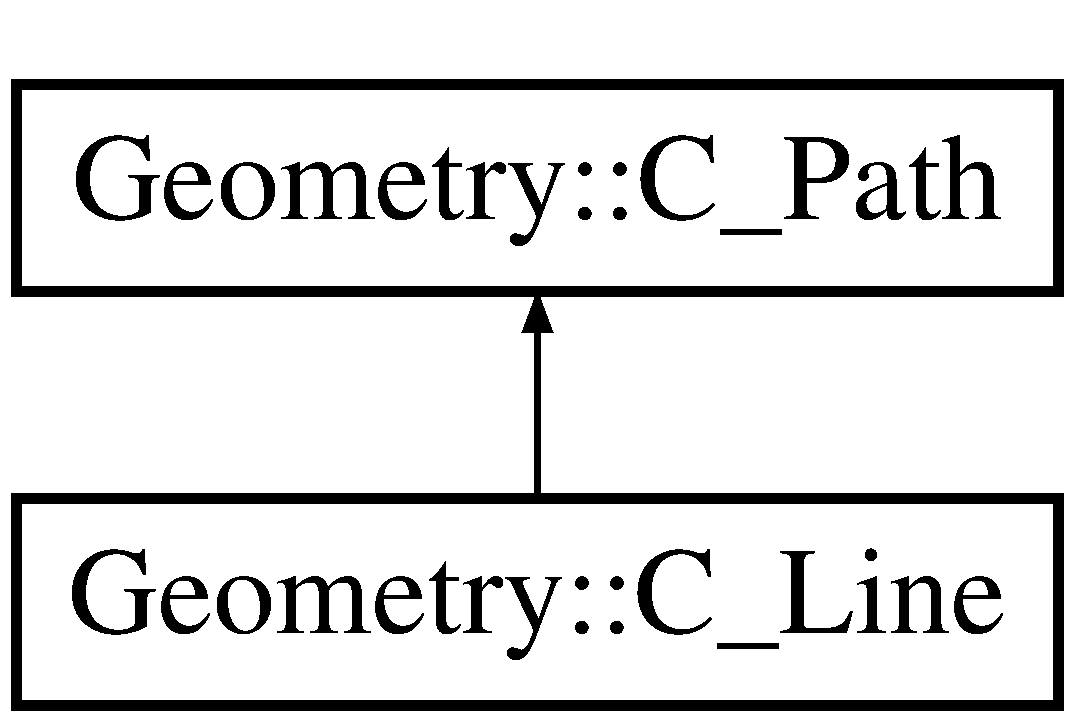
\includegraphics[height=2.000000cm]{class_geometry_1_1_c___line}
\end{center}
\end{figure}
\subsection*{Public Member Functions}
\begin{DoxyCompactItemize}
\item 
\hypertarget{class_geometry_1_1_c___line_a15acedc22ff33f4b92e3aa10d15081ed}{{\bfseries C\-\_\-\-Line} (t\-\_\-cmplx \-\_\-\-\_\-k\-\_\-coeff, t\-\_\-cmplx \-\_\-\-\_\-b\-\_\-coeff)}\label{class_geometry_1_1_c___line_a15acedc22ff33f4b92e3aa10d15081ed}

\item 
\hypertarget{class_geometry_1_1_c___line_a16c50bebf737fc6a12f9605be5c38944}{t\-\_\-cmplx {\bfseries get\-Path\-At} (t\-\_\-cmplx t\-\_\-paramtr)}\label{class_geometry_1_1_c___line_a16c50bebf737fc6a12f9605be5c38944}

\item 
\hypertarget{class_geometry_1_1_c___line_a5d2a8ca944731f6b8d239b9aa52cbfdf}{t\-\_\-cmplx {\bfseries get\-Derivative\-Path\-At} (t\-\_\-cmplx t\-\_\-paramtr)}\label{class_geometry_1_1_c___line_a5d2a8ca944731f6b8d239b9aa52cbfdf}

\end{DoxyCompactItemize}


The documentation for this class was generated from the following files\-:\begin{DoxyCompactItemize}
\item 
source/\-Num\-Libs/\-Geometry/Line.\-hpp\item 
source/\-Num\-Libs/\-Geometry/Line.\-cpp\end{DoxyCompactItemize}

\hypertarget{class_c___memory_factory}{\section{C\-\_\-\-Memory\-Factory Class Reference}
\label{class_c___memory_factory}\index{C\-\_\-\-Memory\-Factory@{C\-\_\-\-Memory\-Factory}}
}
Inheritance diagram for C\-\_\-\-Memory\-Factory\-:\begin{figure}[H]
\begin{center}
\leavevmode
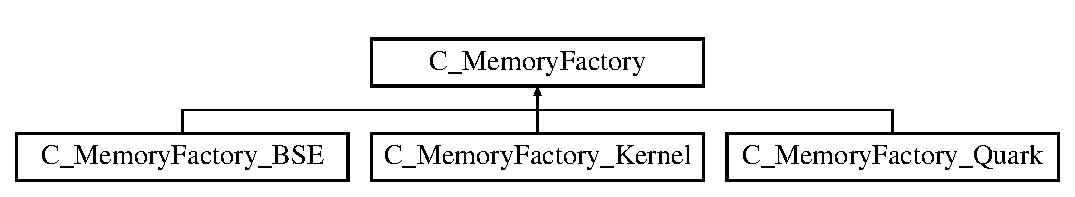
\includegraphics[height=2.000000cm]{class_c___memory_factory}
\end{center}
\end{figure}
\subsection*{Public Member Functions}
\begin{DoxyCompactItemize}
\item 
\hypertarget{class_c___memory_factory_a8d498d5b8573c502ae313b1c1018a098}{virtual \hyperlink{class_c___dedic_mem___abs}{C\-\_\-\-Dedic\-Mem\-\_\-\-Abs} $\ast$ {\bfseries Create\-Memory} ()=0}\label{class_c___memory_factory_a8d498d5b8573c502ae313b1c1018a098}

\end{DoxyCompactItemize}


The documentation for this class was generated from the following file\-:\begin{DoxyCompactItemize}
\item 
source/\-Dedic\-Mem/Memory\-Factories.\-hpp\end{DoxyCompactItemize}

\hypertarget{class_c___memory_factory___b_s_e}{\section{C\-\_\-\-Memory\-Factory\-\_\-\-B\-S\-E Class Reference}
\label{class_c___memory_factory___b_s_e}\index{C\-\_\-\-Memory\-Factory\-\_\-\-B\-S\-E@{C\-\_\-\-Memory\-Factory\-\_\-\-B\-S\-E}}
}


{\ttfamily \#include $<$Memory\-Factories.\-hpp$>$}

\subsection*{Public Member Functions}
\begin{DoxyCompactItemize}
\item 
\hyperlink{class_c___dedic_mem___abs}{C\-\_\-\-Dedic\-Mem\-\_\-\-Abs} $\ast$ \hyperlink{class_c___memory_factory___b_s_e_a75af4c2fa19fd6ccf7f046c323e005c2}{Create\-Memory} ()
\end{DoxyCompactItemize}


\subsection{Member Function Documentation}
\hypertarget{class_c___memory_factory___b_s_e_a75af4c2fa19fd6ccf7f046c323e005c2}{\index{C\-\_\-\-Memory\-Factory\-\_\-\-B\-S\-E@{C\-\_\-\-Memory\-Factory\-\_\-\-B\-S\-E}!Create\-Memory@{Create\-Memory}}
\index{Create\-Memory@{Create\-Memory}!C_MemoryFactory_BSE@{C\-\_\-\-Memory\-Factory\-\_\-\-B\-S\-E}}
\subsubsection[{Create\-Memory}]{\setlength{\rightskip}{0pt plus 5cm}{\bf C\-\_\-\-Dedic\-Mem\-\_\-\-Abs}$\ast$ C\-\_\-\-Memory\-Factory\-\_\-\-B\-S\-E\-::\-Create\-Memory (
\begin{DoxyParamCaption}
{}
\end{DoxyParamCaption}
)\hspace{0.3cm}{\ttfamily [inline]}}}\label{class_c___memory_factory___b_s_e_a75af4c2fa19fd6ccf7f046c323e005c2}


The documentation for this class was generated from the following file\-:\begin{DoxyCompactItemize}
\item 
source/\-Dedic\-Mem/\hyperlink{_memory_factories_8hpp}{Memory\-Factories.\-hpp}\end{DoxyCompactItemize}

\hypertarget{class_c___memory_factory___kernel}{\section{C\-\_\-\-Memory\-Factory\-\_\-\-Kernel Class Reference}
\label{class_c___memory_factory___kernel}\index{C\-\_\-\-Memory\-Factory\-\_\-\-Kernel@{C\-\_\-\-Memory\-Factory\-\_\-\-Kernel}}
}
Inheritance diagram for C\-\_\-\-Memory\-Factory\-\_\-\-Kernel\-:\begin{figure}[H]
\begin{center}
\leavevmode
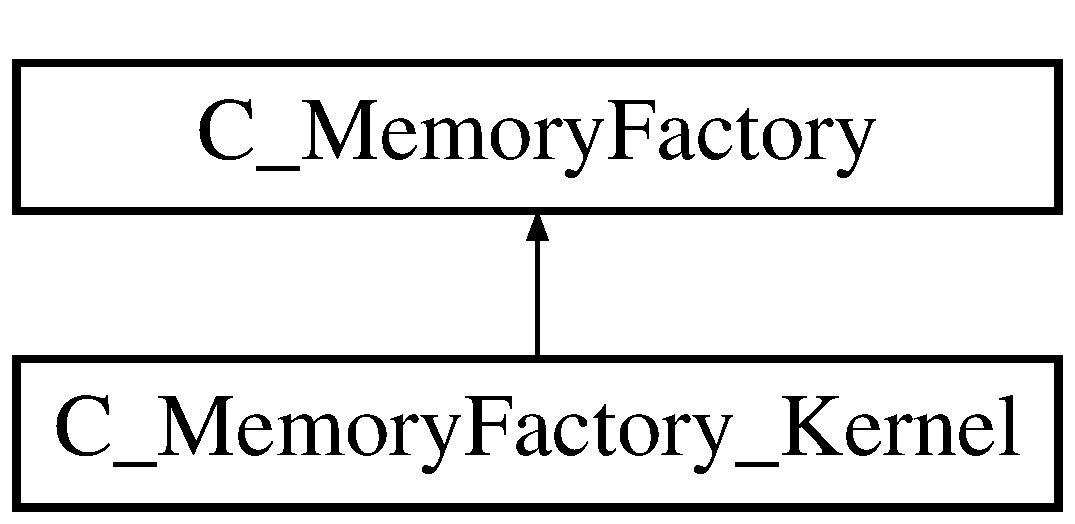
\includegraphics[height=2.000000cm]{class_c___memory_factory___kernel}
\end{center}
\end{figure}
\subsection*{Public Member Functions}
\begin{DoxyCompactItemize}
\item 
\hypertarget{class_c___memory_factory___kernel_ac8741e6e30ed5dad51579507cf7b4007}{\hyperlink{class_c___dedic_mem___abs}{C\-\_\-\-Dedic\-Mem\-\_\-\-Abs} $\ast$ {\bfseries Create\-Memory} ()}\label{class_c___memory_factory___kernel_ac8741e6e30ed5dad51579507cf7b4007}

\end{DoxyCompactItemize}


The documentation for this class was generated from the following file\-:\begin{DoxyCompactItemize}
\item 
source/\-Dedic\-Mem/Memory\-Factories.\-hpp\end{DoxyCompactItemize}

\hypertarget{class_c___memory_factory___quark}{\section{C\-\_\-\-Memory\-Factory\-\_\-\-Quark Class Reference}
\label{class_c___memory_factory___quark}\index{C\-\_\-\-Memory\-Factory\-\_\-\-Quark@{C\-\_\-\-Memory\-Factory\-\_\-\-Quark}}
}
Inheritance diagram for C\-\_\-\-Memory\-Factory\-\_\-\-Quark\-:\begin{figure}[H]
\begin{center}
\leavevmode
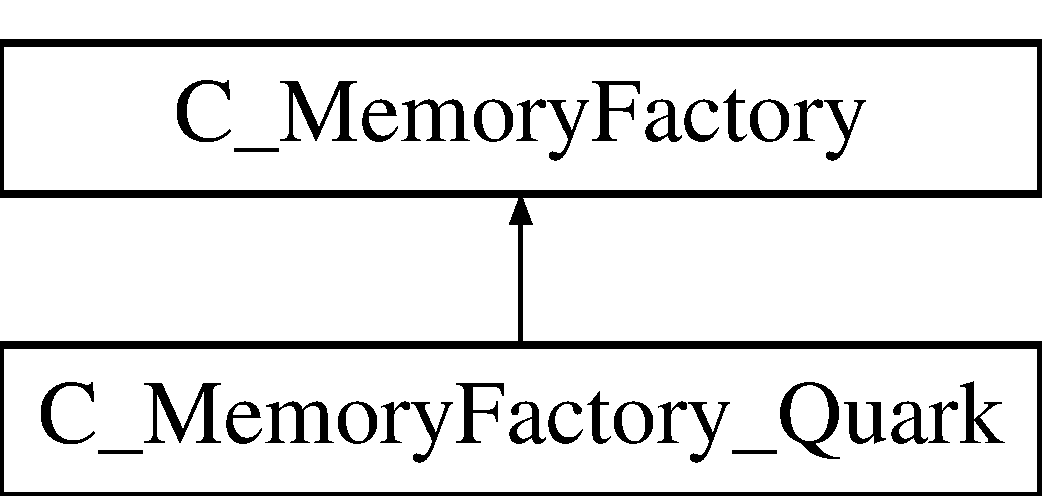
\includegraphics[height=2.000000cm]{class_c___memory_factory___quark}
\end{center}
\end{figure}
\subsection*{Public Member Functions}
\begin{DoxyCompactItemize}
\item 
\hypertarget{class_c___memory_factory___quark_acdd015023349f6658c14cd5f74d1806d}{\hyperlink{class_c___dedic_mem___abs}{C\-\_\-\-Dedic\-Mem\-\_\-\-Abs} $\ast$ {\bfseries Create\-Memory} ()}\label{class_c___memory_factory___quark_acdd015023349f6658c14cd5f74d1806d}

\end{DoxyCompactItemize}


The documentation for this class was generated from the following file\-:\begin{DoxyCompactItemize}
\item 
source/\-Dedic\-Mem/Memory\-Factories.\-hpp\end{DoxyCompactItemize}

\hypertarget{class_c___meson}{\section{C\-\_\-\-Meson Class Reference}
\label{class_c___meson}\index{C\-\_\-\-Meson@{C\-\_\-\-Meson}}
}
Inheritance diagram for C\-\_\-\-Meson\-:\begin{figure}[H]
\begin{center}
\leavevmode
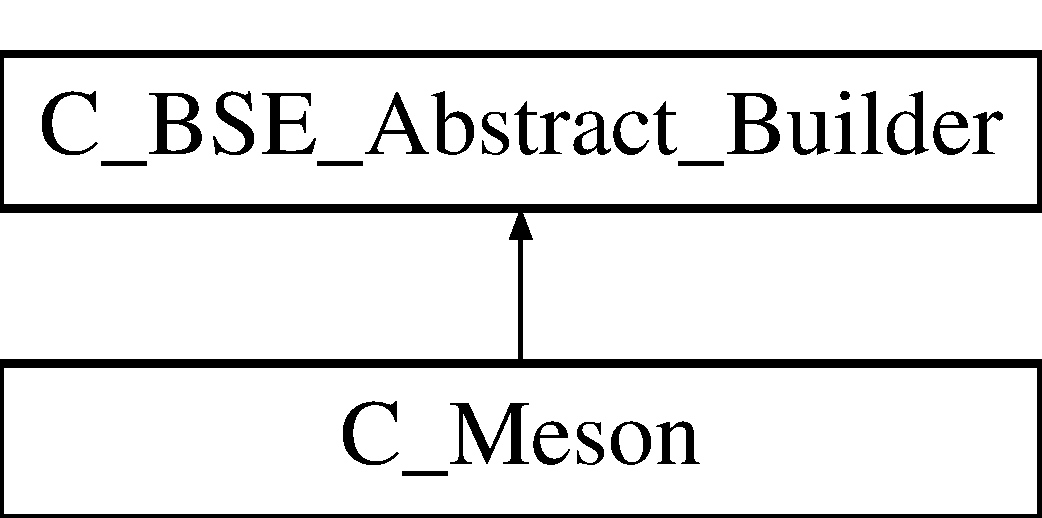
\includegraphics[height=2.000000cm]{class_c___meson}
\end{center}
\end{figure}
\subsection*{Public Member Functions}
\begin{DoxyCompactItemize}
\item 
\hypertarget{class_c___meson_a420efdd72187874a8430d616266833f1}{{\bfseries C\-\_\-\-Meson} (Quark\-\_\-\-I\-D Q1\-\_\-id, Quark\-\_\-\-I\-D Q2\-\_\-id, Kernel\-\_\-\-I\-D K1\-\_\-id, Gluon\-\_\-\-I\-D G1\-\_\-id, P\-S\-\_\-type\-\_\-\-I\-D Ex\-\_\-id)}\label{class_c___meson_a420efdd72187874a8430d616266833f1}

\item 
\hypertarget{class_c___meson_ae21f82fc9162ccc59e38a9eeda1ec51e}{void {\bfseries Symmetric\-Quarks\-Detector} ()}\label{class_c___meson_ae21f82fc9162ccc59e38a9eeda1ec51e}

\item 
\hypertarget{class_c___meson_a7c7a699f66d424cf9903931bba0ee87b}{void {\bfseries build\-Propagators} ()}\label{class_c___meson_a7c7a699f66d424cf9903931bba0ee87b}

\item 
\hypertarget{class_c___meson_ad998f092a112975437273ed65470126e}{void {\bfseries build\-Kernels} ()}\label{class_c___meson_ad998f092a112975437273ed65470126e}

\item 
\hypertarget{class_c___meson_a0fc41cd31216390951ccab66779d47e6}{void {\bfseries build\-B\-S\-Es} ()}\label{class_c___meson_a0fc41cd31216390951ccab66779d47e6}

\item 
\hypertarget{class_c___meson_ad0a7c652dbd7078285002b1153e99bb6}{void {\bfseries Link\-Them\-All} ()}\label{class_c___meson_ad0a7c652dbd7078285002b1153e99bb6}

\end{DoxyCompactItemize}
\subsection*{Public Attributes}
\begin{DoxyCompactItemize}
\item 
\hypertarget{class_c___meson_a300d351aea69188bf790d48643880a27}{Kernel\-\_\-\-I\-D {\bfseries kernel\-\_\-\-I\-D}}\label{class_c___meson_a300d351aea69188bf790d48643880a27}

\item 
\hypertarget{class_c___meson_aec23f4540faa712152b933b6bd4c252e}{Quark\-\_\-\-I\-D {\bfseries quark\-\_\-1\-\_\-\-I\-D}}\label{class_c___meson_aec23f4540faa712152b933b6bd4c252e}

\item 
\hypertarget{class_c___meson_a1e3ab02ec52a316544fc9f5f1be834c7}{Quark\-\_\-\-I\-D {\bfseries quark\-\_\-2\-\_\-\-I\-D}}\label{class_c___meson_a1e3ab02ec52a316544fc9f5f1be834c7}

\item 
\hypertarget{class_c___meson_a43ab30db480af7fadf307b5ce3e8f283}{Gluon\-\_\-\-I\-D {\bfseries gluon\-\_\-\-I\-D}}\label{class_c___meson_a43ab30db480af7fadf307b5ce3e8f283}

\item 
\hypertarget{class_c___meson_a98c581e24aaa3e12ff1f594426c64446}{P\-S\-\_\-type\-\_\-\-I\-D {\bfseries exchange\-\_\-type\-\_\-\-I\-D}}\label{class_c___meson_a98c581e24aaa3e12ff1f594426c64446}

\item 
\hypertarget{class_c___meson_aa2db9e37db36ab471b3b6d863094484e}{std\-::vector$<$ \hyperlink{class_c___propagator}{C\-\_\-\-Propagator} $\ast$ $>$ {\bfseries Propagators}}\label{class_c___meson_aa2db9e37db36ab471b3b6d863094484e}

\item 
\hypertarget{class_c___meson_a5a2cfe858f7a999983e42a42de26cb7d}{std\-::vector$<$ \hyperlink{class_c___abstract_kernel}{C\-\_\-\-Abstract\-Kernel} $\ast$ $>$ {\bfseries Kernels}}\label{class_c___meson_a5a2cfe858f7a999983e42a42de26cb7d}

\item 
\hypertarget{class_c___meson_a98416e65f01449a73e2b12eed01e694a}{std\-::vector$<$ \hyperlink{class_c___b_s_e___hadron___base}{C\-\_\-\-B\-S\-E\-\_\-\-Hadron\-\_\-\-Base} $\ast$ $>$ {\bfseries B\-S\-Es}}\label{class_c___meson_a98416e65f01449a73e2b12eed01e694a}

\end{DoxyCompactItemize}


The documentation for this class was generated from the following file\-:\begin{DoxyCompactItemize}
\item 
source/\-Vertex/\-B\-S\-E/B\-S\-E\-\_\-\-Builder.\-hpp\end{DoxyCompactItemize}

\hypertarget{class_c___mesons___axial_vector}{\section{C\-\_\-\-Mesons\-\_\-\-Axial\-Vector Class Reference}
\label{class_c___mesons___axial_vector}\index{C\-\_\-\-Mesons\-\_\-\-Axial\-Vector@{C\-\_\-\-Mesons\-\_\-\-Axial\-Vector}}
}
Inheritance diagram for C\-\_\-\-Mesons\-\_\-\-Axial\-Vector\-:\begin{figure}[H]
\begin{center}
\leavevmode
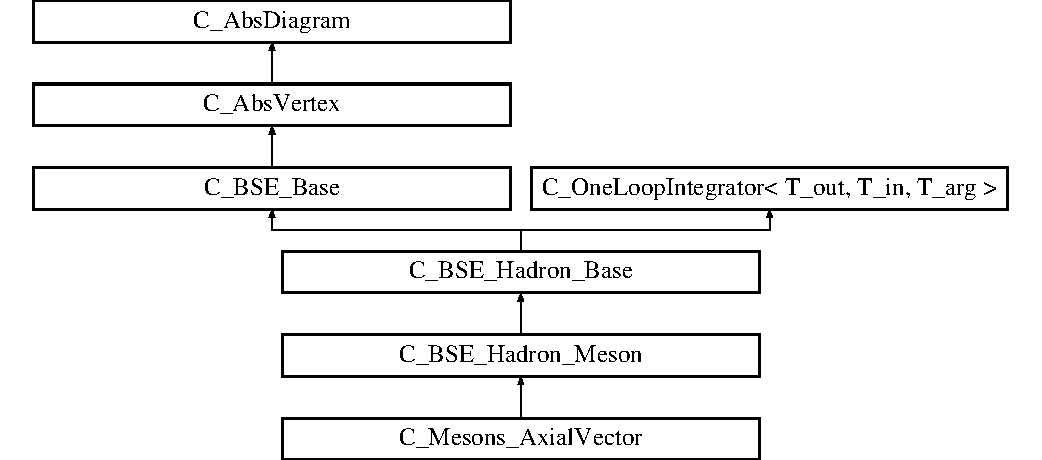
\includegraphics[height=6.000000cm]{class_c___mesons___axial_vector}
\end{center}
\end{figure}
\subsection*{Public Member Functions}
\begin{DoxyCompactItemize}
\item 
\hypertarget{class_c___mesons___axial_vector_add87e06c484c9e115e1510386b2f43fa}{void {\bfseries Set\-Dirac\-Structures} (t\-\_\-cmplx\-Vector \-\_\-k, t\-\_\-cmplx\-Vector \-\_\-\-P, std\-::vector$<$ t\-\_\-cmplx\-Dirac $>$ $\ast$Dirac\-Structure)}\label{class_c___mesons___axial_vector_add87e06c484c9e115e1510386b2f43fa}

\item 
\hypertarget{class_c___mesons___axial_vector_ab997718c834a05ee9bdc015c013d9dcd}{virtual \hyperlink{class_c___mesons___axial_vector}{C\-\_\-\-Mesons\-\_\-\-Axial\-Vector} $\ast$ {\bfseries Make\-Copy} ()}\label{class_c___mesons___axial_vector_ab997718c834a05ee9bdc015c013d9dcd}

\item 
\hypertarget{class_c___mesons___axial_vector_a8c165af2052746923638b1560da9367e}{t\-\_\-cmplx\-Matrix {\bfseries Disentangle\-Amps} (t\-\_\-cmplx\-Matrix $\ast$pre\-\_\-result)}\label{class_c___mesons___axial_vector_a8c165af2052746923638b1560da9367e}

\end{DoxyCompactItemize}
\subsection*{Additional Inherited Members}


The documentation for this class was generated from the following file\-:\begin{DoxyCompactItemize}
\item 
source/\-Vertex/\-B\-S\-E/B\-S\-E\-\_\-\-Mesons.\-hpp\end{DoxyCompactItemize}

\hypertarget{class_c___mesons___pseudo_scalar}{\section{C\-\_\-\-Mesons\-\_\-\-Pseudo\-Scalar Class Reference}
\label{class_c___mesons___pseudo_scalar}\index{C\-\_\-\-Mesons\-\_\-\-Pseudo\-Scalar@{C\-\_\-\-Mesons\-\_\-\-Pseudo\-Scalar}}
}
Inheritance diagram for C\-\_\-\-Mesons\-\_\-\-Pseudo\-Scalar\-:\begin{figure}[H]
\begin{center}
\leavevmode
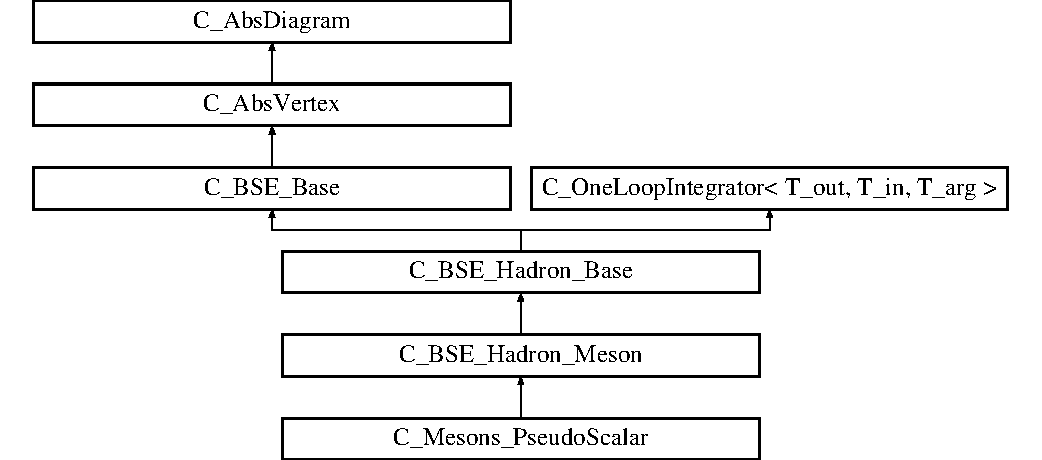
\includegraphics[height=6.000000cm]{class_c___mesons___pseudo_scalar}
\end{center}
\end{figure}
\subsection*{Public Member Functions}
\begin{DoxyCompactItemize}
\item 
\hypertarget{class_c___mesons___pseudo_scalar_a8b0fe6ddc33e67dc0f71877b7b62e66a}{void {\bfseries Set\-Dirac\-Structures} (t\-\_\-cmplx\-Vector \-\_\-k, t\-\_\-cmplx\-Vector \-\_\-\-P, std\-::vector$<$ t\-\_\-cmplx\-Dirac $>$ $\ast$Dirac\-Structure)}\label{class_c___mesons___pseudo_scalar_a8b0fe6ddc33e67dc0f71877b7b62e66a}

\item 
\hypertarget{class_c___mesons___pseudo_scalar_ae1915d7867f2a24a8c8ae4a8a9b1b020}{virtual \hyperlink{class_c___mesons___pseudo_scalar}{C\-\_\-\-Mesons\-\_\-\-Pseudo\-Scalar} $\ast$ {\bfseries Make\-Copy} ()}\label{class_c___mesons___pseudo_scalar_ae1915d7867f2a24a8c8ae4a8a9b1b020}

\item 
\hypertarget{class_c___mesons___pseudo_scalar_ad18d40271977cd2160250f6ef6a30a30}{t\-\_\-cmplx\-Matrix {\bfseries Disentangle\-Amps} (t\-\_\-cmplx\-Matrix $\ast$pre\-\_\-result)}\label{class_c___mesons___pseudo_scalar_ad18d40271977cd2160250f6ef6a30a30}

\end{DoxyCompactItemize}
\subsection*{Additional Inherited Members}


The documentation for this class was generated from the following file\-:\begin{DoxyCompactItemize}
\item 
source/\-Vertex/\-B\-S\-E/B\-S\-E\-\_\-\-Mesons.\-hpp\end{DoxyCompactItemize}

\hypertarget{class_c___mesons___scalar}{\section{C\-\_\-\-Mesons\-\_\-\-Scalar Class Reference}
\label{class_c___mesons___scalar}\index{C\-\_\-\-Mesons\-\_\-\-Scalar@{C\-\_\-\-Mesons\-\_\-\-Scalar}}
}
Inheritance diagram for C\-\_\-\-Mesons\-\_\-\-Scalar\-:\begin{figure}[H]
\begin{center}
\leavevmode
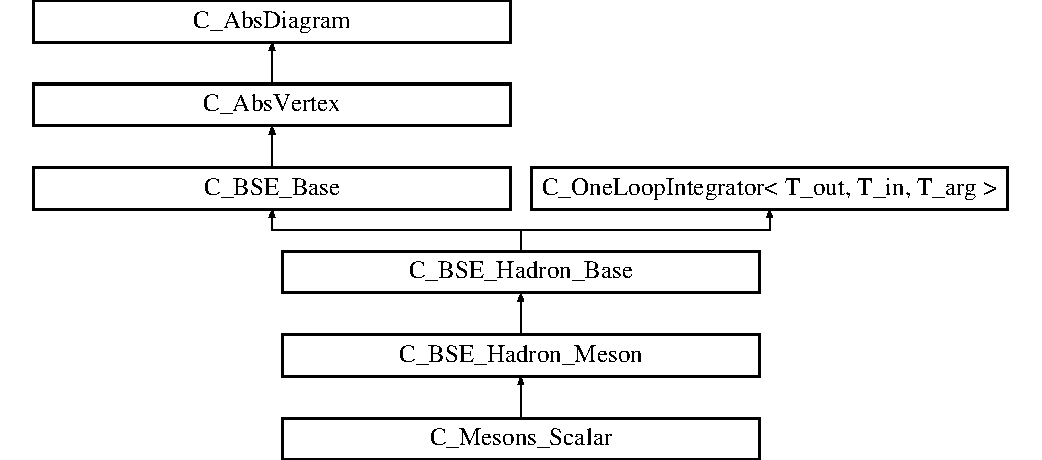
\includegraphics[height=6.000000cm]{class_c___mesons___scalar}
\end{center}
\end{figure}
\subsection*{Public Member Functions}
\begin{DoxyCompactItemize}
\item 
\hypertarget{class_c___mesons___scalar_a2d20b015c874ecef6d0b7f2e128c5486}{void {\bfseries Set\-Dirac\-Structures} (t\-\_\-cmplx\-Vector \-\_\-k, t\-\_\-cmplx\-Vector \-\_\-\-P, std\-::vector$<$ t\-\_\-cmplx\-Dirac $>$ $\ast$Dirac\-Structure)}\label{class_c___mesons___scalar_a2d20b015c874ecef6d0b7f2e128c5486}

\item 
\hypertarget{class_c___mesons___scalar_ab5762566b28886e84e155d85e7586f1a}{virtual \hyperlink{class_c___mesons___scalar}{C\-\_\-\-Mesons\-\_\-\-Scalar} $\ast$ {\bfseries Make\-Copy} ()}\label{class_c___mesons___scalar_ab5762566b28886e84e155d85e7586f1a}

\item 
\hypertarget{class_c___mesons___scalar_a6fc6d0154a13bb88cd52e6367ea851a3}{t\-\_\-cmplx\-Matrix {\bfseries Disentangle\-Amps} (t\-\_\-cmplx\-Matrix $\ast$pre\-\_\-result)}\label{class_c___mesons___scalar_a6fc6d0154a13bb88cd52e6367ea851a3}

\end{DoxyCompactItemize}
\subsection*{Additional Inherited Members}


The documentation for this class was generated from the following file\-:\begin{DoxyCompactItemize}
\item 
source/\-Vertex/\-B\-S\-E/B\-S\-E\-\_\-\-Mesons.\-hpp\end{DoxyCompactItemize}

\hypertarget{class_c___mesons___tensor}{\section{C\-\_\-\-Mesons\-\_\-\-Tensor Class Reference}
\label{class_c___mesons___tensor}\index{C\-\_\-\-Mesons\-\_\-\-Tensor@{C\-\_\-\-Mesons\-\_\-\-Tensor}}
}
Inheritance diagram for C\-\_\-\-Mesons\-\_\-\-Tensor\-:\begin{figure}[H]
\begin{center}
\leavevmode
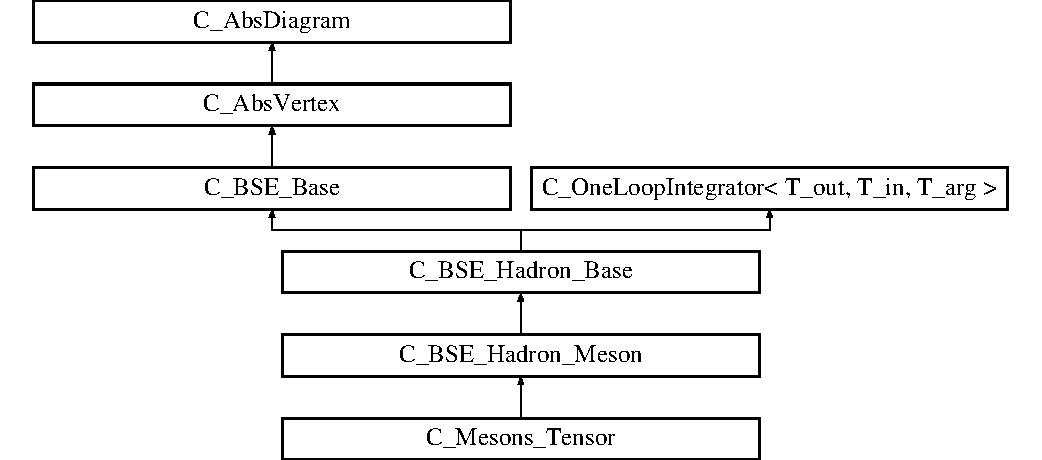
\includegraphics[height=6.000000cm]{class_c___mesons___tensor}
\end{center}
\end{figure}
\subsection*{Public Member Functions}
\begin{DoxyCompactItemize}
\item 
\hypertarget{class_c___mesons___tensor_a04097cb301a1b19622b8dd39f9e3ce0c}{void {\bfseries Set\-Dirac\-Structures} (t\-\_\-cmplx\-Vector \-\_\-k, t\-\_\-cmplx\-Vector \-\_\-\-P, std\-::vector$<$ t\-\_\-cmplx\-Dirac $>$ $\ast$Dirac\-Structure)}\label{class_c___mesons___tensor_a04097cb301a1b19622b8dd39f9e3ce0c}

\item 
\hypertarget{class_c___mesons___tensor_a1710c5be08596588b0a7fcc61d20eb50}{virtual \hyperlink{class_c___mesons___tensor}{C\-\_\-\-Mesons\-\_\-\-Tensor} $\ast$ {\bfseries Make\-Copy} ()}\label{class_c___mesons___tensor_a1710c5be08596588b0a7fcc61d20eb50}

\item 
\hypertarget{class_c___mesons___tensor_a963677c1e4751e6a964a7fd4b7ac1464}{t\-\_\-cmplx\-Matrix {\bfseries Disentangle\-Amps} (t\-\_\-cmplx\-Matrix $\ast$pre\-\_\-result)}\label{class_c___mesons___tensor_a963677c1e4751e6a964a7fd4b7ac1464}

\end{DoxyCompactItemize}
\subsection*{Additional Inherited Members}


The documentation for this class was generated from the following file\-:\begin{DoxyCompactItemize}
\item 
source/\-Vertex/\-B\-S\-E/B\-S\-E\-\_\-\-Mesons.\-hpp\end{DoxyCompactItemize}

\hypertarget{class_c___mesons___vector}{\section{C\-\_\-\-Mesons\-\_\-\-Vector Class Reference}
\label{class_c___mesons___vector}\index{C\-\_\-\-Mesons\-\_\-\-Vector@{C\-\_\-\-Mesons\-\_\-\-Vector}}
}
Inheritance diagram for C\-\_\-\-Mesons\-\_\-\-Vector\-:\begin{figure}[H]
\begin{center}
\leavevmode
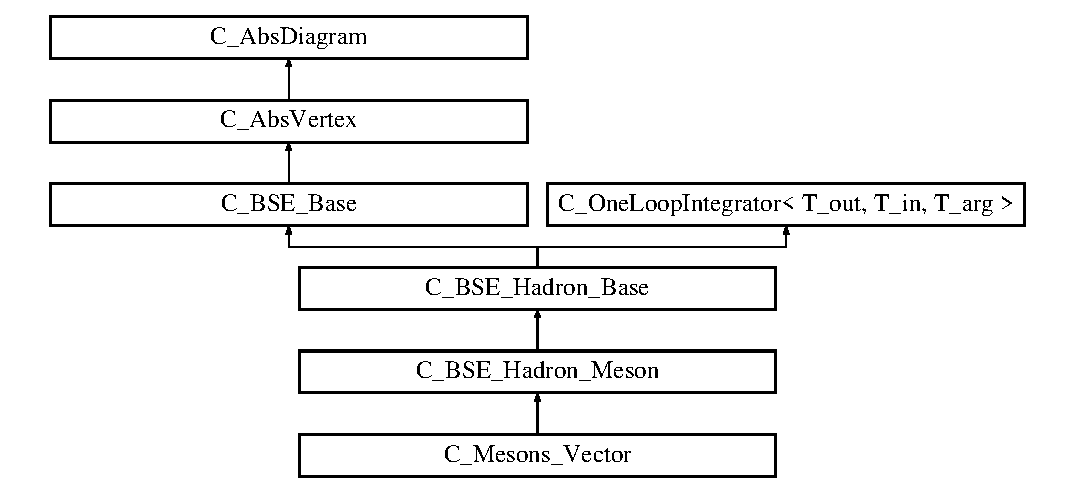
\includegraphics[height=6.000000cm]{class_c___mesons___vector}
\end{center}
\end{figure}
\subsection*{Public Member Functions}
\begin{DoxyCompactItemize}
\item 
\hypertarget{class_c___mesons___vector_a39855d839be872e41a3301c6a137c685}{void {\bfseries Set\-Dirac\-Structures} (t\-\_\-cmplx\-Vector \-\_\-k, t\-\_\-cmplx\-Vector \-\_\-\-P, std\-::vector$<$ t\-\_\-cmplx\-Dirac $>$ $\ast$Dirac\-Structure)}\label{class_c___mesons___vector_a39855d839be872e41a3301c6a137c685}

\item 
\hypertarget{class_c___mesons___vector_a33e74b9c4fbfd2b439137d9e54362dcc}{virtual \hyperlink{class_c___mesons___vector}{C\-\_\-\-Mesons\-\_\-\-Vector} $\ast$ {\bfseries Make\-Copy} ()}\label{class_c___mesons___vector_a33e74b9c4fbfd2b439137d9e54362dcc}

\item 
\hypertarget{class_c___mesons___vector_af0c5781fddc22f3cb91fcbc4bd97a654}{t\-\_\-cmplx\-Matrix {\bfseries Disentangle\-Amps} (t\-\_\-cmplx\-Matrix $\ast$pre\-\_\-result)}\label{class_c___mesons___vector_af0c5781fddc22f3cb91fcbc4bd97a654}

\end{DoxyCompactItemize}
\subsection*{Additional Inherited Members}


The documentation for this class was generated from the following file\-:\begin{DoxyCompactItemize}
\item 
source/\-Vertex/\-B\-S\-E/B\-S\-E\-\_\-\-Mesons.\-hpp\end{DoxyCompactItemize}

\hypertarget{class_c___one_loop_integrator}{\section{C\-\_\-\-One\-Loop\-Integrator$<$ T\-\_\-out, T\-\_\-in, T\-\_\-arg $>$ Class Template Reference}
\label{class_c___one_loop_integrator}\index{C\-\_\-\-One\-Loop\-Integrator$<$ T\-\_\-out, T\-\_\-in, T\-\_\-arg $>$@{C\-\_\-\-One\-Loop\-Integrator$<$ T\-\_\-out, T\-\_\-in, T\-\_\-arg $>$}}
}


{\ttfamily \#include $<$One\-Loop\-Integrator.\-hpp$>$}

\subsection*{Protected Member Functions}
\begin{DoxyCompactItemize}
\item 
\hyperlink{class_c___one_loop_integrator_a2cec9d83b4f5a12b03abf7bd28ef9f72}{C\-\_\-\-One\-Loop\-Integrator} ()
\item 
virtual \hyperlink{class_c___one_loop_integrator_afe89ae625faf097b591fce467e9d1eb5}{$\sim$\-C\-\_\-\-One\-Loop\-Integrator} ()
\item 
T\-\_\-out \hyperlink{class_c___one_loop_integrator_a9dd059711cbac033c88e1ab644ec3084}{calc\-Integral3\-D} (std\-::function$<$ T\-\_\-out(T\-\_\-arg)$>$ $\ast$func\-\_\-to\-\_\-int, int num\-Rows, int num\-Cols)
\item 
T\-\_\-out \hyperlink{class_c___one_loop_integrator_a7b35dcdd6f0f58d305bbaf53ba1afcd4}{calc\-Integral2\-D} (std\-::function$<$ T\-\_\-out(T\-\_\-arg)$>$ $\ast$func\-\_\-to\-\_\-int, int num\-Rows, int num\-Cols)
\end{DoxyCompactItemize}
\subsection*{Protected Attributes}
\begin{DoxyCompactItemize}
\item 
int \hyperlink{class_c___one_loop_integrator_aed8066a37eaa0865bd484ffd18884abb}{num\-Integ\-Dimentions}
\item 
\hyperlink{class_c___integrator___line}{C\-\_\-\-Integrator\-\_\-\-Line}$<$ T\-\_\-out, T\-\_\-in $>$ $\ast$ \hyperlink{class_c___one_loop_integrator_af884706bf7461487cfb254d78b797e94}{Integrator\-\_\-momentum}
\item 
\hyperlink{class_c___integrator___line}{C\-\_\-\-Integrator\-\_\-\-Line}$<$ T\-\_\-out, T\-\_\-in $>$ $\ast$ \hyperlink{class_c___one_loop_integrator_a2826eadcd033a03808d645cd883acceb}{Integrator\-\_\-angle\-\_\-\-Z}
\item 
\hyperlink{class_c___integrator___line}{C\-\_\-\-Integrator\-\_\-\-Line}$<$ T\-\_\-out, T\-\_\-in $>$ $\ast$ \hyperlink{class_c___one_loop_integrator_a5770d28cb44d0ea9c3d331203ee84440}{Integrator\-\_\-angle\-\_\-\-Y}
\item 
std\-::vector$<$ int $>$ \hyperlink{class_c___one_loop_integrator_a78ea7c4afee6c20ed50e6fa171a47dc3}{threadloc\-\_\-\-Integ\-\_\-ctr}
\item 
std\-::vector$<$ int $>$ \hyperlink{class_c___one_loop_integrator_af7ddf02e8c2d913b2a38f6670e26ac3b}{threadloc\-\_\-momentum\-\_\-inx}
\item 
T\-\_\-arg \hyperlink{class_c___one_loop_integrator_a196a8d045623e4af5d4bb9fca7c105bb}{integrand\-\_\-args}
\begin{DoxyCompactList}\small\item\em the variables over the loop integration is done, for example vector $ (k,z,y,\phi) $ \end{DoxyCompactList}\item 
std\-::vector$<$ \hyperlink{class_c___kinematics__1loop}{C\-\_\-\-Kinematics\-\_\-1loop} $>$ \hyperlink{class_c___one_loop_integrator_a767bf7500b35433779ed8b2fdb5b73a7}{threadloc\-\_\-\-Momenta}
\begin{DoxyCompactList}\small\item\em the momenta 4-\/vectors associated with singe loop integration \end{DoxyCompactList}\end{DoxyCompactItemize}


\subsection{Constructor \& Destructor Documentation}
\hypertarget{class_c___one_loop_integrator_a2cec9d83b4f5a12b03abf7bd28ef9f72}{\index{C\-\_\-\-One\-Loop\-Integrator@{C\-\_\-\-One\-Loop\-Integrator}!C\-\_\-\-One\-Loop\-Integrator@{C\-\_\-\-One\-Loop\-Integrator}}
\index{C\-\_\-\-One\-Loop\-Integrator@{C\-\_\-\-One\-Loop\-Integrator}!C_OneLoopIntegrator@{C\-\_\-\-One\-Loop\-Integrator}}
\subsubsection[{C\-\_\-\-One\-Loop\-Integrator}]{\setlength{\rightskip}{0pt plus 5cm}template$<$typename T\-\_\-out, typename T\-\_\-in, typename T\-\_\-arg$>$ {\bf C\-\_\-\-One\-Loop\-Integrator}$<$ T\-\_\-out, T\-\_\-in, T\-\_\-arg $>$\-::{\bf C\-\_\-\-One\-Loop\-Integrator} (
\begin{DoxyParamCaption}
{}
\end{DoxyParamCaption}
)\hspace{0.3cm}{\ttfamily [inline]}, {\ttfamily [protected]}}}\label{class_c___one_loop_integrator_a2cec9d83b4f5a12b03abf7bd28ef9f72}
\hypertarget{class_c___one_loop_integrator_afe89ae625faf097b591fce467e9d1eb5}{\index{C\-\_\-\-One\-Loop\-Integrator@{C\-\_\-\-One\-Loop\-Integrator}!$\sim$\-C\-\_\-\-One\-Loop\-Integrator@{$\sim$\-C\-\_\-\-One\-Loop\-Integrator}}
\index{$\sim$\-C\-\_\-\-One\-Loop\-Integrator@{$\sim$\-C\-\_\-\-One\-Loop\-Integrator}!C_OneLoopIntegrator@{C\-\_\-\-One\-Loop\-Integrator}}
\subsubsection[{$\sim$\-C\-\_\-\-One\-Loop\-Integrator}]{\setlength{\rightskip}{0pt plus 5cm}template$<$typename T\-\_\-out, typename T\-\_\-in, typename T\-\_\-arg$>$ virtual {\bf C\-\_\-\-One\-Loop\-Integrator}$<$ T\-\_\-out, T\-\_\-in, T\-\_\-arg $>$\-::$\sim${\bf C\-\_\-\-One\-Loop\-Integrator} (
\begin{DoxyParamCaption}
{}
\end{DoxyParamCaption}
)\hspace{0.3cm}{\ttfamily [inline]}, {\ttfamily [protected]}, {\ttfamily [virtual]}}}\label{class_c___one_loop_integrator_afe89ae625faf097b591fce467e9d1eb5}


\subsection{Member Function Documentation}
\hypertarget{class_c___one_loop_integrator_a7b35dcdd6f0f58d305bbaf53ba1afcd4}{\index{C\-\_\-\-One\-Loop\-Integrator@{C\-\_\-\-One\-Loop\-Integrator}!calc\-Integral2\-D@{calc\-Integral2\-D}}
\index{calc\-Integral2\-D@{calc\-Integral2\-D}!C_OneLoopIntegrator@{C\-\_\-\-One\-Loop\-Integrator}}
\subsubsection[{calc\-Integral2\-D}]{\setlength{\rightskip}{0pt plus 5cm}template$<$typename T\-\_\-out, typename T\-\_\-in, typename T\-\_\-arg$>$ T\-\_\-out {\bf C\-\_\-\-One\-Loop\-Integrator}$<$ T\-\_\-out, T\-\_\-in, T\-\_\-arg $>$\-::calc\-Integral2\-D (
\begin{DoxyParamCaption}
\item[{std\-::function$<$ T\-\_\-out(T\-\_\-arg)$>$ $\ast$}]{func\-\_\-to\-\_\-int, }
\item[{int}]{num\-Rows, }
\item[{int}]{num\-Cols}
\end{DoxyParamCaption}
)\hspace{0.3cm}{\ttfamily [inline]}, {\ttfamily [protected]}}}\label{class_c___one_loop_integrator_a7b35dcdd6f0f58d305bbaf53ba1afcd4}
\hypertarget{class_c___one_loop_integrator_a9dd059711cbac033c88e1ab644ec3084}{\index{C\-\_\-\-One\-Loop\-Integrator@{C\-\_\-\-One\-Loop\-Integrator}!calc\-Integral3\-D@{calc\-Integral3\-D}}
\index{calc\-Integral3\-D@{calc\-Integral3\-D}!C_OneLoopIntegrator@{C\-\_\-\-One\-Loop\-Integrator}}
\subsubsection[{calc\-Integral3\-D}]{\setlength{\rightskip}{0pt plus 5cm}template$<$typename T\-\_\-out, typename T\-\_\-in, typename T\-\_\-arg$>$ T\-\_\-out {\bf C\-\_\-\-One\-Loop\-Integrator}$<$ T\-\_\-out, T\-\_\-in, T\-\_\-arg $>$\-::calc\-Integral3\-D (
\begin{DoxyParamCaption}
\item[{std\-::function$<$ T\-\_\-out(T\-\_\-arg)$>$ $\ast$}]{func\-\_\-to\-\_\-int, }
\item[{int}]{num\-Rows, }
\item[{int}]{num\-Cols}
\end{DoxyParamCaption}
)\hspace{0.3cm}{\ttfamily [inline]}, {\ttfamily [protected]}}}\label{class_c___one_loop_integrator_a9dd059711cbac033c88e1ab644ec3084}


\subsection{Member Data Documentation}
\hypertarget{class_c___one_loop_integrator_a196a8d045623e4af5d4bb9fca7c105bb}{\index{C\-\_\-\-One\-Loop\-Integrator@{C\-\_\-\-One\-Loop\-Integrator}!integrand\-\_\-args@{integrand\-\_\-args}}
\index{integrand\-\_\-args@{integrand\-\_\-args}!C_OneLoopIntegrator@{C\-\_\-\-One\-Loop\-Integrator}}
\subsubsection[{integrand\-\_\-args}]{\setlength{\rightskip}{0pt plus 5cm}template$<$typename T\-\_\-out, typename T\-\_\-in, typename T\-\_\-arg$>$ T\-\_\-arg {\bf C\-\_\-\-One\-Loop\-Integrator}$<$ T\-\_\-out, T\-\_\-in, T\-\_\-arg $>$\-::integrand\-\_\-args\hspace{0.3cm}{\ttfamily [protected]}}}\label{class_c___one_loop_integrator_a196a8d045623e4af5d4bb9fca7c105bb}


the variables over the loop integration is done, for example vector $ (k,z,y,\phi) $ 

\hypertarget{class_c___one_loop_integrator_a5770d28cb44d0ea9c3d331203ee84440}{\index{C\-\_\-\-One\-Loop\-Integrator@{C\-\_\-\-One\-Loop\-Integrator}!Integrator\-\_\-angle\-\_\-\-Y@{Integrator\-\_\-angle\-\_\-\-Y}}
\index{Integrator\-\_\-angle\-\_\-\-Y@{Integrator\-\_\-angle\-\_\-\-Y}!C_OneLoopIntegrator@{C\-\_\-\-One\-Loop\-Integrator}}
\subsubsection[{Integrator\-\_\-angle\-\_\-\-Y}]{\setlength{\rightskip}{0pt plus 5cm}template$<$typename T\-\_\-out, typename T\-\_\-in, typename T\-\_\-arg$>$ {\bf C\-\_\-\-Integrator\-\_\-\-Line}$<$T\-\_\-out,T\-\_\-in$>$$\ast$ {\bf C\-\_\-\-One\-Loop\-Integrator}$<$ T\-\_\-out, T\-\_\-in, T\-\_\-arg $>$\-::Integrator\-\_\-angle\-\_\-\-Y\hspace{0.3cm}{\ttfamily [protected]}}}\label{class_c___one_loop_integrator_a5770d28cb44d0ea9c3d331203ee84440}
\hypertarget{class_c___one_loop_integrator_a2826eadcd033a03808d645cd883acceb}{\index{C\-\_\-\-One\-Loop\-Integrator@{C\-\_\-\-One\-Loop\-Integrator}!Integrator\-\_\-angle\-\_\-\-Z@{Integrator\-\_\-angle\-\_\-\-Z}}
\index{Integrator\-\_\-angle\-\_\-\-Z@{Integrator\-\_\-angle\-\_\-\-Z}!C_OneLoopIntegrator@{C\-\_\-\-One\-Loop\-Integrator}}
\subsubsection[{Integrator\-\_\-angle\-\_\-\-Z}]{\setlength{\rightskip}{0pt plus 5cm}template$<$typename T\-\_\-out, typename T\-\_\-in, typename T\-\_\-arg$>$ {\bf C\-\_\-\-Integrator\-\_\-\-Line}$<$T\-\_\-out,T\-\_\-in$>$$\ast$ {\bf C\-\_\-\-One\-Loop\-Integrator}$<$ T\-\_\-out, T\-\_\-in, T\-\_\-arg $>$\-::Integrator\-\_\-angle\-\_\-\-Z\hspace{0.3cm}{\ttfamily [protected]}}}\label{class_c___one_loop_integrator_a2826eadcd033a03808d645cd883acceb}
\hypertarget{class_c___one_loop_integrator_af884706bf7461487cfb254d78b797e94}{\index{C\-\_\-\-One\-Loop\-Integrator@{C\-\_\-\-One\-Loop\-Integrator}!Integrator\-\_\-momentum@{Integrator\-\_\-momentum}}
\index{Integrator\-\_\-momentum@{Integrator\-\_\-momentum}!C_OneLoopIntegrator@{C\-\_\-\-One\-Loop\-Integrator}}
\subsubsection[{Integrator\-\_\-momentum}]{\setlength{\rightskip}{0pt plus 5cm}template$<$typename T\-\_\-out, typename T\-\_\-in, typename T\-\_\-arg$>$ {\bf C\-\_\-\-Integrator\-\_\-\-Line}$<$T\-\_\-out,T\-\_\-in$>$$\ast$ {\bf C\-\_\-\-One\-Loop\-Integrator}$<$ T\-\_\-out, T\-\_\-in, T\-\_\-arg $>$\-::Integrator\-\_\-momentum\hspace{0.3cm}{\ttfamily [protected]}}}\label{class_c___one_loop_integrator_af884706bf7461487cfb254d78b797e94}
\hypertarget{class_c___one_loop_integrator_aed8066a37eaa0865bd484ffd18884abb}{\index{C\-\_\-\-One\-Loop\-Integrator@{C\-\_\-\-One\-Loop\-Integrator}!num\-Integ\-Dimentions@{num\-Integ\-Dimentions}}
\index{num\-Integ\-Dimentions@{num\-Integ\-Dimentions}!C_OneLoopIntegrator@{C\-\_\-\-One\-Loop\-Integrator}}
\subsubsection[{num\-Integ\-Dimentions}]{\setlength{\rightskip}{0pt plus 5cm}template$<$typename T\-\_\-out, typename T\-\_\-in, typename T\-\_\-arg$>$ int {\bf C\-\_\-\-One\-Loop\-Integrator}$<$ T\-\_\-out, T\-\_\-in, T\-\_\-arg $>$\-::num\-Integ\-Dimentions\hspace{0.3cm}{\ttfamily [protected]}}}\label{class_c___one_loop_integrator_aed8066a37eaa0865bd484ffd18884abb}
\hypertarget{class_c___one_loop_integrator_a78ea7c4afee6c20ed50e6fa171a47dc3}{\index{C\-\_\-\-One\-Loop\-Integrator@{C\-\_\-\-One\-Loop\-Integrator}!threadloc\-\_\-\-Integ\-\_\-ctr@{threadloc\-\_\-\-Integ\-\_\-ctr}}
\index{threadloc\-\_\-\-Integ\-\_\-ctr@{threadloc\-\_\-\-Integ\-\_\-ctr}!C_OneLoopIntegrator@{C\-\_\-\-One\-Loop\-Integrator}}
\subsubsection[{threadloc\-\_\-\-Integ\-\_\-ctr}]{\setlength{\rightskip}{0pt plus 5cm}template$<$typename T\-\_\-out, typename T\-\_\-in, typename T\-\_\-arg$>$ std\-::vector$<$int$>$ {\bf C\-\_\-\-One\-Loop\-Integrator}$<$ T\-\_\-out, T\-\_\-in, T\-\_\-arg $>$\-::threadloc\-\_\-\-Integ\-\_\-ctr\hspace{0.3cm}{\ttfamily [protected]}}}\label{class_c___one_loop_integrator_a78ea7c4afee6c20ed50e6fa171a47dc3}
\hypertarget{class_c___one_loop_integrator_a767bf7500b35433779ed8b2fdb5b73a7}{\index{C\-\_\-\-One\-Loop\-Integrator@{C\-\_\-\-One\-Loop\-Integrator}!threadloc\-\_\-\-Momenta@{threadloc\-\_\-\-Momenta}}
\index{threadloc\-\_\-\-Momenta@{threadloc\-\_\-\-Momenta}!C_OneLoopIntegrator@{C\-\_\-\-One\-Loop\-Integrator}}
\subsubsection[{threadloc\-\_\-\-Momenta}]{\setlength{\rightskip}{0pt plus 5cm}template$<$typename T\-\_\-out, typename T\-\_\-in, typename T\-\_\-arg$>$ std\-::vector$<${\bf C\-\_\-\-Kinematics\-\_\-1loop}$>$ {\bf C\-\_\-\-One\-Loop\-Integrator}$<$ T\-\_\-out, T\-\_\-in, T\-\_\-arg $>$\-::threadloc\-\_\-\-Momenta\hspace{0.3cm}{\ttfamily [protected]}}}\label{class_c___one_loop_integrator_a767bf7500b35433779ed8b2fdb5b73a7}


the momenta 4-\/vectors associated with singe loop integration 

\hypertarget{class_c___one_loop_integrator_af7ddf02e8c2d913b2a38f6670e26ac3b}{\index{C\-\_\-\-One\-Loop\-Integrator@{C\-\_\-\-One\-Loop\-Integrator}!threadloc\-\_\-momentum\-\_\-inx@{threadloc\-\_\-momentum\-\_\-inx}}
\index{threadloc\-\_\-momentum\-\_\-inx@{threadloc\-\_\-momentum\-\_\-inx}!C_OneLoopIntegrator@{C\-\_\-\-One\-Loop\-Integrator}}
\subsubsection[{threadloc\-\_\-momentum\-\_\-inx}]{\setlength{\rightskip}{0pt plus 5cm}template$<$typename T\-\_\-out, typename T\-\_\-in, typename T\-\_\-arg$>$ std\-::vector$<$int$>$ {\bf C\-\_\-\-One\-Loop\-Integrator}$<$ T\-\_\-out, T\-\_\-in, T\-\_\-arg $>$\-::threadloc\-\_\-momentum\-\_\-inx\hspace{0.3cm}{\ttfamily [protected]}}}\label{class_c___one_loop_integrator_af7ddf02e8c2d913b2a38f6670e26ac3b}


The documentation for this class was generated from the following file\-:\begin{DoxyCompactItemize}
\item 
source/\-Num\-Libs/\hyperlink{_one_loop_integrator_8hpp}{One\-Loop\-Integrator.\-hpp}\end{DoxyCompactItemize}

\hypertarget{class_geometry_1_1_c___parabola}{\section{Geometry\-:\-:C\-\_\-\-Parabola Class Reference}
\label{class_geometry_1_1_c___parabola}\index{Geometry\-::\-C\-\_\-\-Parabola@{Geometry\-::\-C\-\_\-\-Parabola}}
}
Inheritance diagram for Geometry\-:\-:C\-\_\-\-Parabola\-:\begin{figure}[H]
\begin{center}
\leavevmode
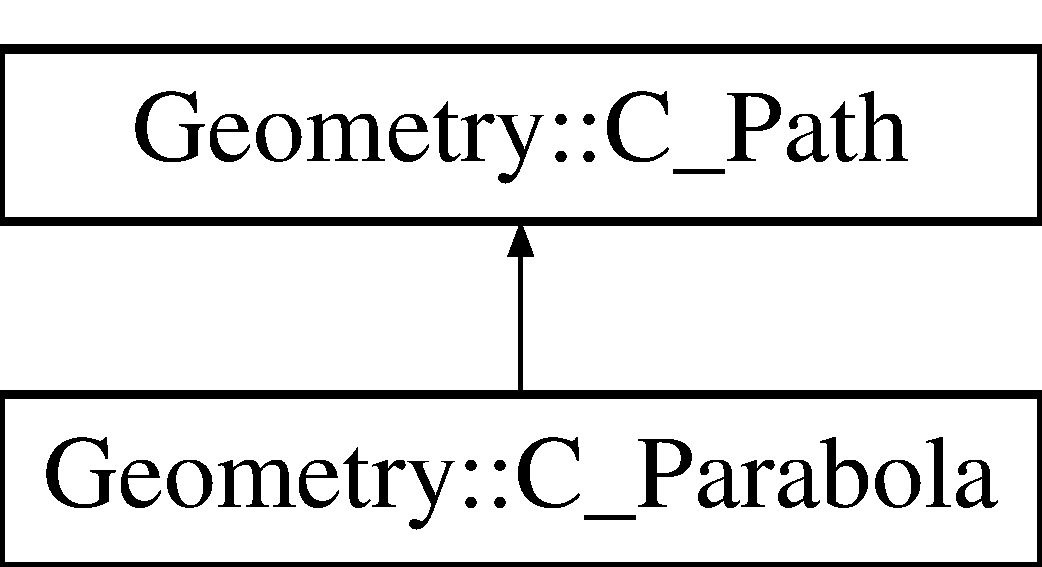
\includegraphics[height=2.000000cm]{class_geometry_1_1_c___parabola}
\end{center}
\end{figure}
\subsection*{Public Member Functions}
\begin{DoxyCompactItemize}
\item 
\hypertarget{class_geometry_1_1_c___parabola_af2dbf3b230334f8c68a116dbe6d21490}{{\bfseries C\-\_\-\-Parabola} (t\-\_\-cmplx \-\_\-\-\_\-\-Parabola\-Apex)}\label{class_geometry_1_1_c___parabola_af2dbf3b230334f8c68a116dbe6d21490}

\item 
\hypertarget{class_geometry_1_1_c___parabola_a387364d860d1fdd83294af454635acb0}{t\-\_\-cmplx {\bfseries get\-Path\-At} (t\-\_\-cmplx t\-\_\-paramtr)}\label{class_geometry_1_1_c___parabola_a387364d860d1fdd83294af454635acb0}

\item 
\hypertarget{class_geometry_1_1_c___parabola_a783b277435ef183353620f94471e3d7d}{t\-\_\-cmplx {\bfseries get\-Derivative\-Path\-At} (t\-\_\-cmplx t\-\_\-paramtr)}\label{class_geometry_1_1_c___parabola_a783b277435ef183353620f94471e3d7d}

\end{DoxyCompactItemize}


The documentation for this class was generated from the following files\-:\begin{DoxyCompactItemize}
\item 
source/\-Num\-Libs/\-Geometry/Parabola.\-hpp\item 
source/\-Num\-Libs/\-Geometry/Parabola.\-cpp\end{DoxyCompactItemize}

\hypertarget{class_geometry_1_1_c___parabola_contour}{\section{Geometry\-:\-:C\-\_\-\-Parabola\-Contour Class Reference}
\label{class_geometry_1_1_c___parabola_contour}\index{Geometry\-::\-C\-\_\-\-Parabola\-Contour@{Geometry\-::\-C\-\_\-\-Parabola\-Contour}}
}
\subsection*{Public Member Functions}
\begin{DoxyCompactItemize}
\item 
\hypertarget{class_geometry_1_1_c___parabola_contour_aa0c00c9315f7d61dd1731074e0846dba}{{\bfseries C\-\_\-\-Parabola\-Contour} (t\-\_\-cmplx \-\_\-\-\_\-\-Parabola\-Apex, t\-\_\-cmplx \-\_\-\-\_\-k\-\_\-coeff, t\-\_\-cmplx \-\_\-\-\_\-b\-\_\-coeff)}\label{class_geometry_1_1_c___parabola_contour_aa0c00c9315f7d61dd1731074e0846dba}

\item 
\hypertarget{class_geometry_1_1_c___parabola_contour_a578b2b2d45be66ef6effe03cbf047a7a}{void {\bfseries set\-Parabola\-Contour} (const t\-\_\-d\-Array1\-D \&p\-\_\-parabola, const t\-\_\-d\-Array1\-D \&w\-\_\-parabola, const t\-\_\-d\-Array1\-D \&p\-\_\-line, const t\-\_\-d\-Array1\-D \&w\-\_\-line)}\label{class_geometry_1_1_c___parabola_contour_a578b2b2d45be66ef6effe03cbf047a7a}

\item 
\hypertarget{class_geometry_1_1_c___parabola_contour_a32867584ce7dfc8234a3446fa803c23f}{t\-\_\-cmplx\-Array2\-D {\bfseries get\-Parabola\-Contour} ()}\label{class_geometry_1_1_c___parabola_contour_a32867584ce7dfc8234a3446fa803c23f}

\end{DoxyCompactItemize}


The documentation for this class was generated from the following files\-:\begin{DoxyCompactItemize}
\item 
source/\-Num\-Libs/\-Geometry/Parabola\-Contour.\-hpp\item 
source/\-Num\-Libs/\-Geometry/Parabola\-Contour.\-cpp\end{DoxyCompactItemize}

\hypertarget{class_geometry_1_1_c___path}{\section{Geometry\-:\-:C\-\_\-\-Path Class Reference}
\label{class_geometry_1_1_c___path}\index{Geometry\-::\-C\-\_\-\-Path@{Geometry\-::\-C\-\_\-\-Path}}
}
Inheritance diagram for Geometry\-:\-:C\-\_\-\-Path\-:\begin{figure}[H]
\begin{center}
\leavevmode
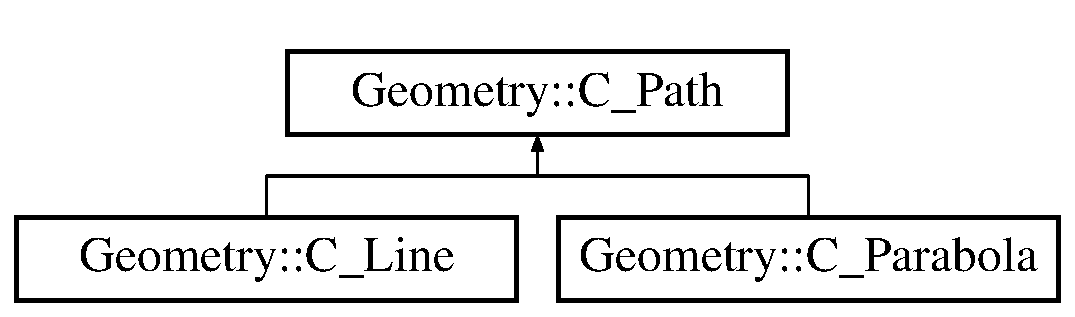
\includegraphics[height=2.000000cm]{class_geometry_1_1_c___path}
\end{center}
\end{figure}
\subsection*{Public Member Functions}
\begin{DoxyCompactItemize}
\item 
\hypertarget{class_geometry_1_1_c___path_a3e09ce3608385b63ebbe9ffad0f0599b}{t\-\_\-cmplx\-Array1\-D {\bfseries get\-Path\-On\-Vector} (t\-\_\-cmplx\-Array1\-D Sample\-Points)}\label{class_geometry_1_1_c___path_a3e09ce3608385b63ebbe9ffad0f0599b}

\item 
\hypertarget{class_geometry_1_1_c___path_a133c937a36b957116043fddfe3fedf46}{virtual t\-\_\-cmplx {\bfseries get\-Path\-At} (t\-\_\-cmplx t\-\_\-paramtr)}\label{class_geometry_1_1_c___path_a133c937a36b957116043fddfe3fedf46}

\item 
\hypertarget{class_geometry_1_1_c___path_a62acb86d6a96d7f0a3185fb498ec449d}{virtual t\-\_\-cmplx {\bfseries get\-Derivative\-Path\-At} (t\-\_\-cmplx t\-\_\-paramtr)}\label{class_geometry_1_1_c___path_a62acb86d6a96d7f0a3185fb498ec449d}

\end{DoxyCompactItemize}


The documentation for this class was generated from the following files\-:\begin{DoxyCompactItemize}
\item 
source/\-Num\-Libs/\-Geometry/Path.\-hpp\item 
source/\-Num\-Libs/\-Geometry/Path.\-cpp\end{DoxyCompactItemize}

\hypertarget{class_c___physical___state}{\section{C\-\_\-\-Physical\-\_\-\-State Class Reference}
\label{class_c___physical___state}\index{C\-\_\-\-Physical\-\_\-\-State@{C\-\_\-\-Physical\-\_\-\-State}}
}
\subsection*{Public Member Functions}
\begin{DoxyCompactItemize}
\item 
\hypertarget{class_c___physical___state_a7c9a16f91504da6fba6c610e6f043ba7}{void {\bfseries Set\-Propagators} (std\-::vector$<$ \hyperlink{class_c___propagator}{C\-\_\-\-Propagator} $\ast$ $>$ \-\_\-\-Propagators)}\label{class_c___physical___state_a7c9a16f91504da6fba6c610e6f043ba7}

\item 
\hypertarget{class_c___physical___state_a9bc4afc2c6aefbac892af2dd8f3b0d5c}{void {\bfseries Set\-Kernels} (std\-::vector$<$ \hyperlink{class_c___abstract_kernel}{C\-\_\-\-Abstract\-Kernel} $\ast$ $>$ \-\_\-\-Kernels)}\label{class_c___physical___state_a9bc4afc2c6aefbac892af2dd8f3b0d5c}

\item 
\hypertarget{class_c___physical___state_abc9444f0b5bcb0f71c951b4cea61c45a}{void {\bfseries Set\-B\-S\-Es} (std\-::vector$<$ \hyperlink{class_c___b_s_e___hadron___base}{C\-\_\-\-B\-S\-E\-\_\-\-Hadron\-\_\-\-Base} $\ast$ $>$ \-\_\-\-B\-S\-Es)}\label{class_c___physical___state_abc9444f0b5bcb0f71c951b4cea61c45a}

\item 
\hypertarget{class_c___physical___state_aa151247bd23165fd5382747cd41d85f4}{void {\bfseries Check\-Pieces} ()}\label{class_c___physical___state_aa151247bd23165fd5382747cd41d85f4}

\end{DoxyCompactItemize}
\subsection*{Public Attributes}
\begin{DoxyCompactItemize}
\item 
\hypertarget{class_c___physical___state_a6640b0fbf6c6f4e49a92c4306bb3b348}{std\-::vector$<$ \hyperlink{class_c___propagator}{C\-\_\-\-Propagator} $\ast$ $>$ {\bfseries Propagators}}\label{class_c___physical___state_a6640b0fbf6c6f4e49a92c4306bb3b348}

\item 
\hypertarget{class_c___physical___state_aad6f9f3512e0daf39b18cec650222bb3}{std\-::vector$<$ \hyperlink{class_c___abstract_kernel}{C\-\_\-\-Abstract\-Kernel} $\ast$ $>$ {\bfseries Kernels}}\label{class_c___physical___state_aad6f9f3512e0daf39b18cec650222bb3}

\item 
\hypertarget{class_c___physical___state_ac6e3d6b9f17b0065316d54928cf6e747}{std\-::vector$<$ \hyperlink{class_c___b_s_e___hadron___base}{C\-\_\-\-B\-S\-E\-\_\-\-Hadron\-\_\-\-Base} $\ast$ $>$ {\bfseries B\-S\-Es}}\label{class_c___physical___state_ac6e3d6b9f17b0065316d54928cf6e747}

\end{DoxyCompactItemize}
\subsection*{Friends}
\begin{DoxyCompactItemize}
\item 
\hypertarget{class_c___physical___state_a2dae0cc9b2c5e453b211d44393071b36}{class {\bfseries C\-\_\-\-Manipulator}}\label{class_c___physical___state_a2dae0cc9b2c5e453b211d44393071b36}

\end{DoxyCompactItemize}


The documentation for this class was generated from the following file\-:\begin{DoxyCompactItemize}
\item 
source/\-Vertex/\-B\-S\-E/B\-S\-E\-\_\-\-Builder.\-hpp\end{DoxyCompactItemize}

\hypertarget{class_c___propagator}{\section{C\-\_\-\-Propagator Class Reference}
\label{class_c___propagator}\index{C\-\_\-\-Propagator@{C\-\_\-\-Propagator}}
}
Inheritance diagram for C\-\_\-\-Propagator\-:\begin{figure}[H]
\begin{center}
\leavevmode
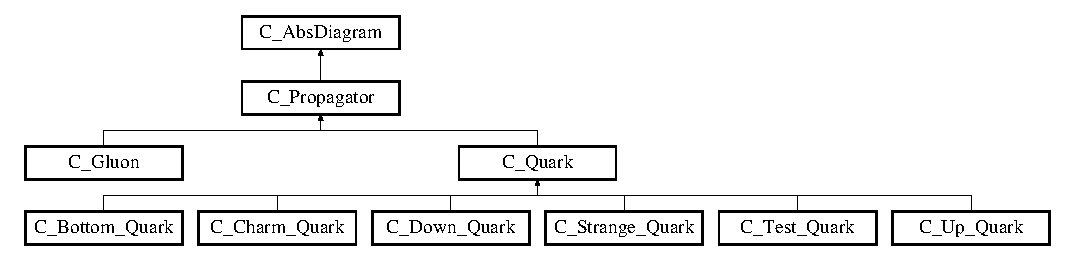
\includegraphics[height=3.060109cm]{class_c___propagator}
\end{center}
\end{figure}
\subsection*{Public Member Functions}
\begin{DoxyCompactItemize}
\item 
virtual void \hyperlink{class_c___propagator_a4b82db59060878e794c3590ee3fbc3f1}{dress\-Propagator} ()=0
\item 
virtual void \hyperlink{class_c___propagator_a2efb521f2afd9ad94c07f62db1d03b8b}{set\-To\-Initial\-State} ()=0
\item 
virtual t\-\_\-cmplx\-Array1\-D \hyperlink{class_c___propagator_a7bf057f408c2a30667fffea12d1375ba}{Propagator\-At\-Point} (t\-\_\-cmplx q)
\item 
virtual void \hyperlink{class_c___propagator_a47d173c63a0256ad71f41fd1cf873d4d}{Set\-Propagator\-On\-Path} (std\-::vector$<$ t\-\_\-cmplx\-Matrix $>$ \&Amplitudes\-On\-Path, t\-\_\-cmplx\-Array1\-D \&Path)
\item 
\hypertarget{class_c___propagator_a5b9292b9ec6396c95238255cb9116727}{virtual t\-\_\-cmplx {\bfseries Dressing\-Factor} ()}\label{class_c___propagator_a5b9292b9ec6396c95238255cb9116727}

\item 
\hypertarget{class_c___propagator_ac607b22d1dbb5c947606182b36acab54}{virtual void {\bfseries set\-Contour\-Apex} (double M2)}\label{class_c___propagator_ac607b22d1dbb5c947606182b36acab54}

\item 
\hypertarget{class_c___propagator_a6b49ff6bc2a98001966e987dc7d9230a}{virtual double {\bfseries check\-Sum} ()}\label{class_c___propagator_a6b49ff6bc2a98001966e987dc7d9230a}

\item 
\hypertarget{class_c___propagator_ad278336169262f85686e400feed87750}{virtual void {\bfseries link\-To\-Kernel} (\hyperlink{class_c___abstract_kernel}{C\-\_\-\-Abstract\-Kernel} $\ast$\-\_\-\-K)}\label{class_c___propagator_ad278336169262f85686e400feed87750}

\end{DoxyCompactItemize}
\subsection*{Additional Inherited Members}


\subsection{Member Function Documentation}
\hypertarget{class_c___propagator_a4b82db59060878e794c3590ee3fbc3f1}{\index{C\-\_\-\-Propagator@{C\-\_\-\-Propagator}!dress\-Propagator@{dress\-Propagator}}
\index{dress\-Propagator@{dress\-Propagator}!C_Propagator@{C\-\_\-\-Propagator}}
\subsubsection[{dress\-Propagator}]{\setlength{\rightskip}{0pt plus 5cm}virtual void C\-\_\-\-Propagator\-::dress\-Propagator (
\begin{DoxyParamCaption}
{}
\end{DoxyParamCaption}
)\hspace{0.3cm}{\ttfamily [pure virtual]}}}\label{class_c___propagator_a4b82db59060878e794c3590ee3fbc3f1}
Dress Propagator according to defined in derived class D\-S\-E scheme this is the function where all !!\-S\-C\-I\-E\-N\-C\-E!! of D\-S\-E happens 

Implemented in \hyperlink{class_c___quark_a9ab0f782b3d722eea50544e1101c00c5}{C\-\_\-\-Quark}.

\hypertarget{class_c___propagator_a7bf057f408c2a30667fffea12d1375ba}{\index{C\-\_\-\-Propagator@{C\-\_\-\-Propagator}!Propagator\-At\-Point@{Propagator\-At\-Point}}
\index{Propagator\-At\-Point@{Propagator\-At\-Point}!C_Propagator@{C\-\_\-\-Propagator}}
\subsubsection[{Propagator\-At\-Point}]{\setlength{\rightskip}{0pt plus 5cm}t\-\_\-cmplx\-Array1\-D C\-\_\-\-Propagator\-::\-Propagator\-At\-Point (
\begin{DoxyParamCaption}
\item[{t\-\_\-cmplx}]{q}
\end{DoxyParamCaption}
)\hspace{0.3cm}{\ttfamily [virtual]}}}\label{class_c___propagator_a7bf057f408c2a30667fffea12d1375ba}
Return the value of all possible for this kind of propagator dressing functions at point 

Reimplemented in \hyperlink{class_c___quark_a3d1f0eafbded04e910a6576e6a9a079a}{C\-\_\-\-Quark}.

\hypertarget{class_c___propagator_a47d173c63a0256ad71f41fd1cf873d4d}{\index{C\-\_\-\-Propagator@{C\-\_\-\-Propagator}!Set\-Propagator\-On\-Path@{Set\-Propagator\-On\-Path}}
\index{Set\-Propagator\-On\-Path@{Set\-Propagator\-On\-Path}!C_Propagator@{C\-\_\-\-Propagator}}
\subsubsection[{Set\-Propagator\-On\-Path}]{\setlength{\rightskip}{0pt plus 5cm}void C\-\_\-\-Propagator\-::\-Set\-Propagator\-On\-Path (
\begin{DoxyParamCaption}
\item[{std\-::vector$<$ t\-\_\-cmplx\-Matrix $>$ \&}]{Amplitudes\-On\-Path, }
\item[{t\-\_\-cmplx\-Array1\-D \&}]{Path}
\end{DoxyParamCaption}
)\hspace{0.3cm}{\ttfamily [virtual]}}}\label{class_c___propagator_a47d173c63a0256ad71f41fd1cf873d4d}
Save propagator dressing functions, evaluated on provided \char`\"{}\-Path\char`\"{}, in provided \char`\"{}\-Amplitude\-Storage\char`\"{} \hypertarget{class_c___propagator_a2efb521f2afd9ad94c07f62db1d03b8b}{\index{C\-\_\-\-Propagator@{C\-\_\-\-Propagator}!set\-To\-Initial\-State@{set\-To\-Initial\-State}}
\index{set\-To\-Initial\-State@{set\-To\-Initial\-State}!C_Propagator@{C\-\_\-\-Propagator}}
\subsubsection[{set\-To\-Initial\-State}]{\setlength{\rightskip}{0pt plus 5cm}virtual void C\-\_\-\-Propagator\-::set\-To\-Initial\-State (
\begin{DoxyParamCaption}
{}
\end{DoxyParamCaption}
)\hspace{0.3cm}{\ttfamily [pure virtual]}}}\label{class_c___propagator_a2efb521f2afd9ad94c07f62db1d03b8b}
Reset parameters to initial values 

Implemented in \hyperlink{class_c___quark_afe212ef0b9b354ce78670323f3110633}{C\-\_\-\-Quark}.



The documentation for this class was generated from the following files\-:\begin{DoxyCompactItemize}
\item 
source/\-D\-S\-E/Propagator.\-hpp\item 
source/\-D\-S\-E/Propagator.\-cpp\end{DoxyCompactItemize}

\hypertarget{class_c___propagator___factory}{\section{C\-\_\-\-Propagator\-\_\-\-Factory Class Reference}
\label{class_c___propagator___factory}\index{C\-\_\-\-Propagator\-\_\-\-Factory@{C\-\_\-\-Propagator\-\_\-\-Factory}}
}
Inheritance diagram for C\-\_\-\-Propagator\-\_\-\-Factory\-:\begin{figure}[H]
\begin{center}
\leavevmode
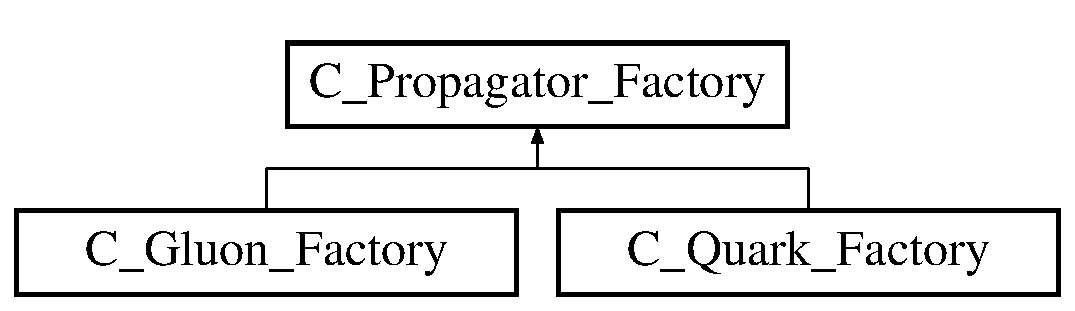
\includegraphics[height=2.000000cm]{class_c___propagator___factory}
\end{center}
\end{figure}
\subsection*{Public Member Functions}
\begin{DoxyCompactItemize}
\item 
\hypertarget{class_c___propagator___factory_aa795aee44b7c0e9b0cf737e9acc1b47b}{virtual \hyperlink{class_c___propagator}{C\-\_\-\-Propagator} $\ast$ {\bfseries Create} (int)=0}\label{class_c___propagator___factory_aa795aee44b7c0e9b0cf737e9acc1b47b}

\end{DoxyCompactItemize}


The documentation for this class was generated from the following file\-:\begin{DoxyCompactItemize}
\item 
source/\-D\-S\-E/Propagator\-Factory.\-hpp\end{DoxyCompactItemize}

\hypertarget{class_c___quark}{\section{C\-\_\-\-Quark Class Reference}
\label{class_c___quark}\index{C\-\_\-\-Quark@{C\-\_\-\-Quark}}
}


{\ttfamily \#include $<$Quark.\-hpp$>$}

Inheritance diagram for C\-\_\-\-Quark\-:\begin{figure}[H]
\begin{center}
\leavevmode
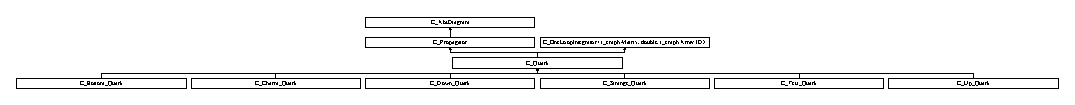
\includegraphics[height=0.957265cm]{class_c___quark}
\end{center}
\end{figure}
\subsection*{Protected Member Functions}
\begin{DoxyCompactItemize}
\item 
\hyperlink{class_c___quark_a7ceb205746e82ecf1c792ec9f11c037a}{C\-\_\-\-Quark} ()
\item 
\hyperlink{class_c___quark_a49f6931861a7144c7215abdbcfba0b7d}{$\sim$\-C\-\_\-\-Quark} ()
\item 
\hypertarget{class_c___quark_aea358bb9c82c6e62d99c69893cc35cf9}{void {\bfseries link\-To\-Kernel} (\hyperlink{class_c___abstract_kernel}{C\-\_\-\-Abstract\-Kernel} $\ast$\-\_\-\-K)}\label{class_c___quark_aea358bb9c82c6e62d99c69893cc35cf9}

\item 
\hypertarget{class_c___quark_a8705085256b1afed49a029e7566be3a6}{void {\bfseries read\-Quark\-Parameters} (string \&\-\_\-\-Param\-Path)}\label{class_c___quark_a8705085256b1afed49a029e7566be3a6}

\item 
\hypertarget{class_c___quark_a08c1d6a09388082de04c981e8106caa1}{t\-\_\-cmplx {\bfseries Dressing\-Factor} ()}\label{class_c___quark_a08c1d6a09388082de04c981e8106caa1}

\item 
\hypertarget{class_c___quark_a1065f0f828e3d7766c8c04f83277d77b}{void {\bfseries set\-Contour\-Apex} (double M2)}\label{class_c___quark_a1065f0f828e3d7766c8c04f83277d77b}

\item 
void \hyperlink{class_c___quark_afe212ef0b9b354ce78670323f3110633}{set\-To\-Initial\-State} ()
\item 
void \hyperlink{class_c___quark_aff74305e3c468db6ec6cbd63e04fff9a}{initializate\-Integrators} ()
\item 
void \hyperlink{class_c___quark_a569aee23f1aafca5fe383ad4341df8e8}{resize\-Memory} ()
\item 
void \hyperlink{class_c___quark_a56f87c010401c5cd211cdd3edd53b2a0}{set\-Contour} ()
\item 
void \hyperlink{class_c___quark_aa5f4509e09ec22aae258b25dbf1cb328}{set\-Grid} ()
\item 
void \hyperlink{class_c___quark_a9bd2e345fa3034850454c5eae8ca585a}{set\-Initial\-Aand\-B} ()
\item 
t\-\_\-cmplx\-Array1\-D \hyperlink{class_c___quark_a80d1fb9d4107a67eae72c87e3653e7ef}{Propagator\-On\-Point} (t\-\_\-cmplx coordin)
\item 
void \hyperlink{class_c___quark_aed45d2fb4598cbb55b3fef5edcc6e826}{calc\-Prop\-On\-Grid} ()
\item 
void \hyperlink{class_c___quark_abade7bfefe26cdb91a1d8a8583879fff}{calc\-Prop\-On\-Contour} ()
\item 
void \hyperlink{class_c___quark_a3aa1d8e442cd1e051ed8e1deb37868e0}{set\-Kinematic} (t\-\_\-cmplx\-Vector \&k, t\-\_\-cmplx\-Vector \&p, t\-\_\-cmplx x, t\-\_\-cmplx y, t\-\_\-cmplx z)
\item 
t\-\_\-cmplx\-Matrix \hyperlink{class_c___quark_a9f6b8538c2c1b9af29a5c063b26ec7d8}{Integrand\-\_\-numerical} (t\-\_\-cmplx\-Array1\-D values)
\item 
t\-\_\-cmplx\-Array1\-D \hyperlink{class_c___quark_a3d1f0eafbded04e910a6576e6a9a079a}{Propagator\-At\-Point} (t\-\_\-cmplx q)
\item 
void \hyperlink{class_c___quark_a6e76c6b1d863858beed18f1c0d9e41d1}{calc\-Propagator} ()
\item 
void \hyperlink{class_c___quark_a5dc9671be863cde85f57705caaf11ee6}{renormalize\-Prop} ()
\item 
double \hyperlink{class_c___quark_ae755b4cd41dd4ce1a6dfd1c432d01bd1}{check\-Convergence} (double previous\-\_\-checksum)
\item 
void \hyperlink{class_c___quark_a9ab0f782b3d722eea50544e1101c00c5}{dress\-Propagator} ()
\item 
void \hyperlink{class_c___quark_af6aebddc61fe85aaf454e459d3de6283}{draw\-On\-Real\-Axis} (int s)
\item 
void \hyperlink{class_c___quark_a53d6cb2219f3a6deb67e6ba85aba8f92}{save\-Propagator} ()
\item 
void \hyperlink{class_c___quark_afff9ac6d9f21b6d3656c1a0e380f9327}{load\-Propagator} ()
\item 
void \hyperlink{class_c___quark_a998f5c9e3ee4920aae7f86e2b1e0c179}{export\-Propagator} ()
\item 
void \hyperlink{class_c___quark_aa1a0d2d4817feb9a53ee3d14754586d7}{set\-Propagator\-On\-Path} (std\-::vector$<$ t\-\_\-cmplx\-Matrix $>$ \&Amplitudes, t\-\_\-cmplx\-Array1\-D \&Path)
\item 
double \hyperlink{class_c___quark_a044cb5ab7b63cca9d4d18792634f5bf1}{check\-Sum} ()
\end{DoxyCompactItemize}
\subsection*{Protected Attributes}
\begin{DoxyCompactItemize}
\item 
\hypertarget{class_c___quark_a825f0f4638fa87322db6af8335d6f05b}{\hyperlink{class_c___abstract_kernel}{C\-\_\-\-Abstract\-Kernel} $\ast$ \hyperlink{class_c___quark_a825f0f4638fa87322db6af8335d6f05b}{Kernel}}\label{class_c___quark_a825f0f4638fa87322db6af8335d6f05b}

\begin{DoxyCompactList}\small\item\em two-\/body scattering Kernel \end{DoxyCompactList}\item 
\hypertarget{class_c___quark_a9eb8b047110e9217c8dc615c9938566c}{\hyperlink{class_c___dedic_mem___quark}{C\-\_\-\-Dedic\-Mem\-\_\-\-Quark} $\ast$ \hyperlink{class_c___quark_a9eb8b047110e9217c8dc615c9938566c}{Memory}}\label{class_c___quark_a9eb8b047110e9217c8dc615c9938566c}

\begin{DoxyCompactList}\small\item\em quark's Memory handler class, contains the contour and the grid at which quark D\-S\-E evaluated \end{DoxyCompactList}\item 
\hypertarget{class_c___quark_a6658a59e332c14057398ba12ad2eb36b}{string \hyperlink{class_c___quark_a6658a59e332c14057398ba12ad2eb36b}{Save\-Prop\-Path}}\label{class_c___quark_a6658a59e332c14057398ba12ad2eb36b}

\begin{DoxyCompactList}\small\item\em path to file to store the calculated propagator \end{DoxyCompactList}\item 
\hypertarget{class_c___quark_a9b47aa812f3e3abf90acfb570ae51617}{int \hyperlink{class_c___quark_a9b47aa812f3e3abf90acfb570ae51617}{num\-\_\-amplitudes}}\label{class_c___quark_a9b47aa812f3e3abf90acfb570ae51617}

\begin{DoxyCompactList}\small\item\em number of projected out amplitudes (quark has two, A and B) \end{DoxyCompactList}\item 
\hypertarget{class_c___quark_aa973622070edbcb2e2e8bf12425a4277}{\hyperlink{class_c___quark__parameters}{C\-\_\-\-Quark\-\_\-parameters} \hyperlink{class_c___quark_aa973622070edbcb2e2e8bf12425a4277}{params}}\label{class_c___quark_aa973622070edbcb2e2e8bf12425a4277}

\begin{DoxyCompactList}\small\item\em contains all params the quark D\-S\-E need to have \end{DoxyCompactList}\item 
\hypertarget{class_c___quark_a1dbb8f78522434bceefdb7b42aa1c96c}{std\-::function$<$ t\-\_\-cmplx(t\-\_\-cmplx, \\*
t\-\_\-cmplx)$>$ \hyperlink{class_c___quark_a1dbb8f78522434bceefdb7b42aa1c96c}{Cauchy\-Integraton\-Weight\-\_\-lambda}}\label{class_c___quark_a1dbb8f78522434bceefdb7b42aa1c96c}

\begin{DoxyCompactList}\small\item\em defines the Cauchy integral measure \end{DoxyCompactList}\item 
\hypertarget{class_c___quark_a551a3fc5de8f8b4d8bcb2502b503df41}{\hyperlink{class_c___integrator___line}{C\-\_\-\-Integrator\-\_\-\-Line}\\*
$<$ t\-\_\-cmplx\-Matrix, double $>$ $\ast$ \hyperlink{class_c___quark_a551a3fc5de8f8b4d8bcb2502b503df41}{Integrator\-\_\-momentum\-\_\-cutoff}}\label{class_c___quark_a551a3fc5de8f8b4d8bcb2502b503df41}

\begin{DoxyCompactList}\small\item\em Line Integrator for the cutoff part of parabolic contour. \end{DoxyCompactList}\item 
\hypertarget{class_c___quark_aaa4541680e33e880aa95591e9df3be44}{\hyperlink{class_c___integrator___path}{C\-\_\-\-Integrator\-\_\-\-Path}$<$ t\-\_\-cmplx, \\*
t\-\_\-cmplx\-Array2\-D, t\-\_\-cmplx $>$ $\ast$ \hyperlink{class_c___quark_aaa4541680e33e880aa95591e9df3be44}{Integrator\-\_\-cauchy}}\label{class_c___quark_aaa4541680e33e880aa95591e9df3be44}

\begin{DoxyCompactList}\small\item\em Path Integrator for the complete contour. \end{DoxyCompactList}\item 
\hypertarget{class_c___quark_a6e1d141d7f38aba34e48fd51f4da95de}{t\-\_\-d\-Array1\-D \hyperlink{class_c___quark_a6e1d141d7f38aba34e48fd51f4da95de}{zz\-\_\-radial}}\label{class_c___quark_a6e1d141d7f38aba34e48fd51f4da95de}

\begin{DoxyCompactList}\small\item\em zz are the integration nodes, w are the weights \end{DoxyCompactList}\item 
\hypertarget{class_c___quark_a0b5346b639ac43652861f2210a73676b}{t\-\_\-d\-Array1\-D {\bfseries w\-\_\-radial}}\label{class_c___quark_a0b5346b639ac43652861f2210a73676b}

\item 
\hypertarget{class_c___quark_a30161deac15ede23a568a44bb34f7f71}{t\-\_\-d\-Array1\-D {\bfseries zz\-\_\-cutoff}}\label{class_c___quark_a30161deac15ede23a568a44bb34f7f71}

\item 
\hypertarget{class_c___quark_a79b610a65184ef9c49ee0f3947154dd2}{t\-\_\-d\-Array1\-D {\bfseries w\-\_\-cutoff}}\label{class_c___quark_a79b610a65184ef9c49ee0f3947154dd2}

\item 
\hypertarget{class_c___quark_ae52242e8abf3bb67f88ca271960eeab4}{t\-\_\-d\-Array1\-D {\bfseries zz\-\_\-angle}}\label{class_c___quark_ae52242e8abf3bb67f88ca271960eeab4}

\item 
\hypertarget{class_c___quark_a5a5d2e8dd42a3990344fce6be1667ca4}{t\-\_\-d\-Array1\-D {\bfseries w\-\_\-angle}}\label{class_c___quark_a5a5d2e8dd42a3990344fce6be1667ca4}

\item 
\hypertarget{class_c___quark_ad668099da3ad48b3adf1c2df771cb62c}{double \hyperlink{class_c___quark_ad668099da3ad48b3adf1c2df771cb62c}{kinematic\-Factor}}\label{class_c___quark_ad668099da3ad48b3adf1c2df771cb62c}

\begin{DoxyCompactList}\small\item\em just a momentum volume factor \end{DoxyCompactList}\item 
\hypertarget{class_c___quark_a3bcdcd4f5f0e106f159542b782044b31}{double \hyperlink{class_c___quark_a3bcdcd4f5f0e106f159542b782044b31}{B\-\_\-renorm}}\label{class_c___quark_a3bcdcd4f5f0e106f159542b782044b31}

\begin{DoxyCompactList}\small\item\em Renormalization constants. \end{DoxyCompactList}\item 
\hypertarget{class_c___quark_aaa7b2b26853f8405c2b9b293d2c18a64}{double {\bfseries B\-\_\-mu}}\label{class_c___quark_aaa7b2b26853f8405c2b9b293d2c18a64}

\item 
\hypertarget{class_c___quark_ac5de0438d1b19d8a7f7509efff53b978}{double {\bfseries A\-\_\-renorm}}\label{class_c___quark_ac5de0438d1b19d8a7f7509efff53b978}

\item 
\hypertarget{class_c___quark_ae05f046433b0143198cf37dd0294236c}{double {\bfseries Z2}}\label{class_c___quark_ae05f046433b0143198cf37dd0294236c}

\item 
\hypertarget{class_c___quark_a16276524396db70cf500004e4732b62e}{vector$<$ int $>$ \hyperlink{class_c___quark_a16276524396db70cf500004e4732b62e}{threadloc\-\_\-p\-\_\-momenta\-\_\-inx}}\label{class_c___quark_a16276524396db70cf500004e4732b62e}

\begin{DoxyCompactList}\small\item\em thread-\/local storages of indexes \end{DoxyCompactList}\item 
\hypertarget{class_c___quark_a96dfb638401816915fc1728cb4587f2a}{vector$<$ int $>$ {\bfseries threadloc\-\_\-integr\-\_\-inx}}\label{class_c___quark_a96dfb638401816915fc1728cb4587f2a}

\item 
\hypertarget{class_c___quark_a88da2d4e54ff2d0194691e9ebf0313cc}{bool {\bfseries flag\-\_\-dressed}}\label{class_c___quark_a88da2d4e54ff2d0194691e9ebf0313cc}

\item 
\hypertarget{class_c___quark_ab74616977c12b63b1bb3937656b2a580}{bool {\bfseries flag\-\_\-renormalization}}\label{class_c___quark_ab74616977c12b63b1bb3937656b2a580}

\end{DoxyCompactItemize}
\subsection*{Additional Inherited Members}


\subsection{Detailed Description}
\hyperlink{_quark_8hpp_source}{Quark.\-hpp} Author\-: stkubr 

\subsection{Constructor \& Destructor Documentation}
\hypertarget{class_c___quark_a7ceb205746e82ecf1c792ec9f11c037a}{\index{C\-\_\-\-Quark@{C\-\_\-\-Quark}!C\-\_\-\-Quark@{C\-\_\-\-Quark}}
\index{C\-\_\-\-Quark@{C\-\_\-\-Quark}!C_Quark@{C\-\_\-\-Quark}}
\subsubsection[{C\-\_\-\-Quark}]{\setlength{\rightskip}{0pt plus 5cm}C\-\_\-\-Quark\-::\-C\-\_\-\-Quark (
\begin{DoxyParamCaption}
{}
\end{DoxyParamCaption}
)\hspace{0.3cm}{\ttfamily [protected]}}}\label{class_c___quark_a7ceb205746e82ecf1c792ec9f11c037a}
the constructor \hypertarget{class_c___quark_a49f6931861a7144c7215abdbcfba0b7d}{\index{C\-\_\-\-Quark@{C\-\_\-\-Quark}!$\sim$\-C\-\_\-\-Quark@{$\sim$\-C\-\_\-\-Quark}}
\index{$\sim$\-C\-\_\-\-Quark@{$\sim$\-C\-\_\-\-Quark}!C_Quark@{C\-\_\-\-Quark}}
\subsubsection[{$\sim$\-C\-\_\-\-Quark}]{\setlength{\rightskip}{0pt plus 5cm}C\-\_\-\-Quark\-::$\sim$\-C\-\_\-\-Quark (
\begin{DoxyParamCaption}
{}
\end{DoxyParamCaption}
)\hspace{0.3cm}{\ttfamily [protected]}}}\label{class_c___quark_a49f6931861a7144c7215abdbcfba0b7d}
the destructor 

\subsection{Member Function Documentation}
\hypertarget{class_c___quark_a6e76c6b1d863858beed18f1c0d9e41d1}{\index{C\-\_\-\-Quark@{C\-\_\-\-Quark}!calc\-Propagator@{calc\-Propagator}}
\index{calc\-Propagator@{calc\-Propagator}!C_Quark@{C\-\_\-\-Quark}}
\subsubsection[{calc\-Propagator}]{\setlength{\rightskip}{0pt plus 5cm}void C\-\_\-\-Quark\-::calc\-Propagator (
\begin{DoxyParamCaption}
{}
\end{DoxyParamCaption}
)\hspace{0.3cm}{\ttfamily [protected]}}}\label{class_c___quark_a6e76c6b1d863858beed18f1c0d9e41d1}
Calculate consequently Grid and Contour until converge \hypertarget{class_c___quark_abade7bfefe26cdb91a1d8a8583879fff}{\index{C\-\_\-\-Quark@{C\-\_\-\-Quark}!calc\-Prop\-On\-Contour@{calc\-Prop\-On\-Contour}}
\index{calc\-Prop\-On\-Contour@{calc\-Prop\-On\-Contour}!C_Quark@{C\-\_\-\-Quark}}
\subsubsection[{calc\-Prop\-On\-Contour}]{\setlength{\rightskip}{0pt plus 5cm}void C\-\_\-\-Quark\-::calc\-Prop\-On\-Contour (
\begin{DoxyParamCaption}
{}
\end{DoxyParamCaption}
)\hspace{0.3cm}{\ttfamily [protected]}}}\label{class_c___quark_abade7bfefe26cdb91a1d8a8583879fff}
Obtains quark propagator on the contour by evaluating D\-S\-E integral equations on the grid \hypertarget{class_c___quark_aed45d2fb4598cbb55b3fef5edcc6e826}{\index{C\-\_\-\-Quark@{C\-\_\-\-Quark}!calc\-Prop\-On\-Grid@{calc\-Prop\-On\-Grid}}
\index{calc\-Prop\-On\-Grid@{calc\-Prop\-On\-Grid}!C_Quark@{C\-\_\-\-Quark}}
\subsubsection[{calc\-Prop\-On\-Grid}]{\setlength{\rightskip}{0pt plus 5cm}void C\-\_\-\-Quark\-::calc\-Prop\-On\-Grid (
\begin{DoxyParamCaption}
{}
\end{DoxyParamCaption}
)\hspace{0.3cm}{\ttfamily [protected]}}}\label{class_c___quark_aed45d2fb4598cbb55b3fef5edcc6e826}
Obtains quark propagator on the grid by evaluating Cauchy integral on the contour \hypertarget{class_c___quark_ae755b4cd41dd4ce1a6dfd1c432d01bd1}{\index{C\-\_\-\-Quark@{C\-\_\-\-Quark}!check\-Convergence@{check\-Convergence}}
\index{check\-Convergence@{check\-Convergence}!C_Quark@{C\-\_\-\-Quark}}
\subsubsection[{check\-Convergence}]{\setlength{\rightskip}{0pt plus 5cm}double C\-\_\-\-Quark\-::check\-Convergence (
\begin{DoxyParamCaption}
\item[{double}]{previous\-\_\-checksum}
\end{DoxyParamCaption}
)\hspace{0.3cm}{\ttfamily [protected]}}}\label{class_c___quark_ae755b4cd41dd4ce1a6dfd1c432d01bd1}
Check convergence calculates the difference between current checksum and previous iteration \hypertarget{class_c___quark_a044cb5ab7b63cca9d4d18792634f5bf1}{\index{C\-\_\-\-Quark@{C\-\_\-\-Quark}!check\-Sum@{check\-Sum}}
\index{check\-Sum@{check\-Sum}!C_Quark@{C\-\_\-\-Quark}}
\subsubsection[{check\-Sum}]{\setlength{\rightskip}{0pt plus 5cm}double C\-\_\-\-Quark\-::check\-Sum (
\begin{DoxyParamCaption}
{}
\end{DoxyParamCaption}
)\hspace{0.3cm}{\ttfamily [protected]}, {\ttfamily [virtual]}}}\label{class_c___quark_a044cb5ab7b63cca9d4d18792634f5bf1}
Calculates sum A $\ast$ B functions at 100 points. 

Reimplemented from \hyperlink{class_c___propagator}{C\-\_\-\-Propagator}.

\hypertarget{class_c___quark_af6aebddc61fe85aaf454e459d3de6283}{\index{C\-\_\-\-Quark@{C\-\_\-\-Quark}!draw\-On\-Real\-Axis@{draw\-On\-Real\-Axis}}
\index{draw\-On\-Real\-Axis@{draw\-On\-Real\-Axis}!C_Quark@{C\-\_\-\-Quark}}
\subsubsection[{draw\-On\-Real\-Axis}]{\setlength{\rightskip}{0pt plus 5cm}void C\-\_\-\-Quark\-::draw\-On\-Real\-Axis (
\begin{DoxyParamCaption}
\item[{int}]{s}
\end{DoxyParamCaption}
)\hspace{0.3cm}{\ttfamily [protected]}}}\label{class_c___quark_af6aebddc61fe85aaf454e459d3de6283}
Draw Propagator at real line \hypertarget{class_c___quark_a9ab0f782b3d722eea50544e1101c00c5}{\index{C\-\_\-\-Quark@{C\-\_\-\-Quark}!dress\-Propagator@{dress\-Propagator}}
\index{dress\-Propagator@{dress\-Propagator}!C_Quark@{C\-\_\-\-Quark}}
\subsubsection[{dress\-Propagator}]{\setlength{\rightskip}{0pt plus 5cm}void C\-\_\-\-Quark\-::dress\-Propagator (
\begin{DoxyParamCaption}
{}
\end{DoxyParamCaption}
)\hspace{0.3cm}{\ttfamily [protected]}, {\ttfamily [virtual]}}}\label{class_c___quark_a9ab0f782b3d722eea50544e1101c00c5}
Dress Propagator meaning to solve the quark D\-S\-E iteratively 

Implements \hyperlink{class_c___propagator_a4b82db59060878e794c3590ee3fbc3f1}{C\-\_\-\-Propagator}.

\hypertarget{class_c___quark_a998f5c9e3ee4920aae7f86e2b1e0c179}{\index{C\-\_\-\-Quark@{C\-\_\-\-Quark}!export\-Propagator@{export\-Propagator}}
\index{export\-Propagator@{export\-Propagator}!C_Quark@{C\-\_\-\-Quark}}
\subsubsection[{export\-Propagator}]{\setlength{\rightskip}{0pt plus 5cm}void C\-\_\-\-Quark\-::export\-Propagator (
\begin{DoxyParamCaption}
{}
\end{DoxyParamCaption}
)\hspace{0.3cm}{\ttfamily [protected]}}}\label{class_c___quark_a998f5c9e3ee4920aae7f86e2b1e0c179}
Export Propagator to file (exports all what is needed to perform Cauchy integration outside of this library\-: contour, weights, etc.) \hypertarget{class_c___quark_aff74305e3c468db6ec6cbd63e04fff9a}{\index{C\-\_\-\-Quark@{C\-\_\-\-Quark}!initializate\-Integrators@{initializate\-Integrators}}
\index{initializate\-Integrators@{initializate\-Integrators}!C_Quark@{C\-\_\-\-Quark}}
\subsubsection[{initializate\-Integrators}]{\setlength{\rightskip}{0pt plus 5cm}void C\-\_\-\-Quark\-::initializate\-Integrators (
\begin{DoxyParamCaption}
{}
\end{DoxyParamCaption}
)\hspace{0.3cm}{\ttfamily [protected]}}}\label{class_c___quark_aff74305e3c468db6ec6cbd63e04fff9a}
Create Integrators and get the integration points and weights out of them \hypertarget{class_c___quark_a9f6b8538c2c1b9af29a5c063b26ec7d8}{\index{C\-\_\-\-Quark@{C\-\_\-\-Quark}!Integrand\-\_\-numerical@{Integrand\-\_\-numerical}}
\index{Integrand\-\_\-numerical@{Integrand\-\_\-numerical}!C_Quark@{C\-\_\-\-Quark}}
\subsubsection[{Integrand\-\_\-numerical}]{\setlength{\rightskip}{0pt plus 5cm}t\-\_\-cmplx\-Matrix C\-\_\-\-Quark\-::\-Integrand\-\_\-numerical (
\begin{DoxyParamCaption}
\item[{t\-\_\-cmplx\-Array1\-D}]{integ\-Variables}
\end{DoxyParamCaption}
)\hspace{0.3cm}{\ttfamily [protected]}}}\label{class_c___quark_a9f6b8538c2c1b9af29a5c063b26ec7d8}
Numerical form of the Integrand for quark D\-S\-E (suitable for general Kernel) \hypertarget{class_c___quark_afff9ac6d9f21b6d3656c1a0e380f9327}{\index{C\-\_\-\-Quark@{C\-\_\-\-Quark}!load\-Propagator@{load\-Propagator}}
\index{load\-Propagator@{load\-Propagator}!C_Quark@{C\-\_\-\-Quark}}
\subsubsection[{load\-Propagator}]{\setlength{\rightskip}{0pt plus 5cm}void C\-\_\-\-Quark\-::load\-Propagator (
\begin{DoxyParamCaption}
{}
\end{DoxyParamCaption}
)\hspace{0.3cm}{\ttfamily [protected]}}}\label{class_c___quark_afff9ac6d9f21b6d3656c1a0e380f9327}
Read Propagator from file \hypertarget{class_c___quark_a3d1f0eafbded04e910a6576e6a9a079a}{\index{C\-\_\-\-Quark@{C\-\_\-\-Quark}!Propagator\-At\-Point@{Propagator\-At\-Point}}
\index{Propagator\-At\-Point@{Propagator\-At\-Point}!C_Quark@{C\-\_\-\-Quark}}
\subsubsection[{Propagator\-At\-Point}]{\setlength{\rightskip}{0pt plus 5cm}t\-\_\-cmplx\-Array1\-D C\-\_\-\-Quark\-::\-Propagator\-At\-Point (
\begin{DoxyParamCaption}
\item[{t\-\_\-cmplx}]{q}
\end{DoxyParamCaption}
)\hspace{0.3cm}{\ttfamily [protected]}, {\ttfamily [virtual]}}}\label{class_c___quark_a3d1f0eafbded04e910a6576e6a9a079a}
Calculation A,B,M,Sigma\-\_\-\-V,Sigma\-\_\-\-S at point inside a contour 

Reimplemented from \hyperlink{class_c___propagator_a7bf057f408c2a30667fffea12d1375ba}{C\-\_\-\-Propagator}.

\hypertarget{class_c___quark_a80d1fb9d4107a67eae72c87e3653e7ef}{\index{C\-\_\-\-Quark@{C\-\_\-\-Quark}!Propagator\-On\-Point@{Propagator\-On\-Point}}
\index{Propagator\-On\-Point@{Propagator\-On\-Point}!C_Quark@{C\-\_\-\-Quark}}
\subsubsection[{Propagator\-On\-Point}]{\setlength{\rightskip}{0pt plus 5cm}t\-\_\-cmplx\-Array1\-D C\-\_\-\-Quark\-::\-Propagator\-On\-Point (
\begin{DoxyParamCaption}
\item[{t\-\_\-cmplx}]{coordin}
\end{DoxyParamCaption}
)\hspace{0.3cm}{\ttfamily [protected]}}}\label{class_c___quark_a80d1fb9d4107a67eae72c87e3653e7ef}
Returns the values A and B at point in complex plane by evaluating Cauchy integral on contour \hypertarget{class_c___quark_a5dc9671be863cde85f57705caaf11ee6}{\index{C\-\_\-\-Quark@{C\-\_\-\-Quark}!renormalize\-Prop@{renormalize\-Prop}}
\index{renormalize\-Prop@{renormalize\-Prop}!C_Quark@{C\-\_\-\-Quark}}
\subsubsection[{renormalize\-Prop}]{\setlength{\rightskip}{0pt plus 5cm}void C\-\_\-\-Quark\-::renormalize\-Prop (
\begin{DoxyParamCaption}
{}
\end{DoxyParamCaption}
)\hspace{0.3cm}{\ttfamily [protected]}}}\label{class_c___quark_a5dc9671be863cde85f57705caaf11ee6}
Renormalize A and B quark dressing functions at point params.\-mu \hypertarget{class_c___quark_a569aee23f1aafca5fe383ad4341df8e8}{\index{C\-\_\-\-Quark@{C\-\_\-\-Quark}!resize\-Memory@{resize\-Memory}}
\index{resize\-Memory@{resize\-Memory}!C_Quark@{C\-\_\-\-Quark}}
\subsubsection[{resize\-Memory}]{\setlength{\rightskip}{0pt plus 5cm}void C\-\_\-\-Quark\-::resize\-Memory (
\begin{DoxyParamCaption}
{}
\end{DoxyParamCaption}
)\hspace{0.3cm}{\ttfamily [protected]}}}\label{class_c___quark_a569aee23f1aafca5fe383ad4341df8e8}
Resize the dedicated memory storages for the contour and the grid according to loaded \char`\"{}params\char`\"{} \hypertarget{class_c___quark_a53d6cb2219f3a6deb67e6ba85aba8f92}{\index{C\-\_\-\-Quark@{C\-\_\-\-Quark}!save\-Propagator@{save\-Propagator}}
\index{save\-Propagator@{save\-Propagator}!C_Quark@{C\-\_\-\-Quark}}
\subsubsection[{save\-Propagator}]{\setlength{\rightskip}{0pt plus 5cm}void C\-\_\-\-Quark\-::save\-Propagator (
\begin{DoxyParamCaption}
{}
\end{DoxyParamCaption}
)\hspace{0.3cm}{\ttfamily [protected]}}}\label{class_c___quark_a53d6cb2219f3a6deb67e6ba85aba8f92}
Write Propagator to file \hypertarget{class_c___quark_a56f87c010401c5cd211cdd3edd53b2a0}{\index{C\-\_\-\-Quark@{C\-\_\-\-Quark}!set\-Contour@{set\-Contour}}
\index{set\-Contour@{set\-Contour}!C_Quark@{C\-\_\-\-Quark}}
\subsubsection[{set\-Contour}]{\setlength{\rightskip}{0pt plus 5cm}void C\-\_\-\-Quark\-::set\-Contour (
\begin{DoxyParamCaption}
{}
\end{DoxyParamCaption}
)\hspace{0.3cm}{\ttfamily [protected]}}}\label{class_c___quark_a56f87c010401c5cd211cdd3edd53b2a0}
Set Contour in complex plane the contour is a parabola along real axis with an apex (-\/params.\-M2\-\_\-contour,0), cutted at \char`\"{}params.\-Lim\-Uk\char`\"{} in U\-V. \hypertarget{class_c___quark_aa5f4509e09ec22aae258b25dbf1cb328}{\index{C\-\_\-\-Quark@{C\-\_\-\-Quark}!set\-Grid@{set\-Grid}}
\index{set\-Grid@{set\-Grid}!C_Quark@{C\-\_\-\-Quark}}
\subsubsection[{set\-Grid}]{\setlength{\rightskip}{0pt plus 5cm}void C\-\_\-\-Quark\-::set\-Grid (
\begin{DoxyParamCaption}
{}
\end{DoxyParamCaption}
)\hspace{0.3cm}{\ttfamily [protected]}}}\label{class_c___quark_aa5f4509e09ec22aae258b25dbf1cb328}
Set Grid in complex plane equation for the grid is (p -\/ k)$^\wedge$2, where p$^\wedge$2 in the contour and k is integration momentum in D\-S\-E \hypertarget{class_c___quark_a9bd2e345fa3034850454c5eae8ca585a}{\index{C\-\_\-\-Quark@{C\-\_\-\-Quark}!set\-Initial\-Aand\-B@{set\-Initial\-Aand\-B}}
\index{set\-Initial\-Aand\-B@{set\-Initial\-Aand\-B}!C_Quark@{C\-\_\-\-Quark}}
\subsubsection[{set\-Initial\-Aand\-B}]{\setlength{\rightskip}{0pt plus 5cm}void C\-\_\-\-Quark\-::set\-Initial\-Aand\-B (
\begin{DoxyParamCaption}
{}
\end{DoxyParamCaption}
)\hspace{0.3cm}{\ttfamily [protected]}}}\label{class_c___quark_a9bd2e345fa3034850454c5eae8ca585a}
Initial guesses for A and B \hypertarget{class_c___quark_a3aa1d8e442cd1e051ed8e1deb37868e0}{\index{C\-\_\-\-Quark@{C\-\_\-\-Quark}!set\-Kinematic@{set\-Kinematic}}
\index{set\-Kinematic@{set\-Kinematic}!C_Quark@{C\-\_\-\-Quark}}
\subsubsection[{set\-Kinematic}]{\setlength{\rightskip}{0pt plus 5cm}void C\-\_\-\-Quark\-::set\-Kinematic (
\begin{DoxyParamCaption}
\item[{t\-\_\-cmplx\-Vector \&}]{k, }
\item[{t\-\_\-cmplx\-Vector \&}]{p, }
\item[{t\-\_\-cmplx}]{x, }
\item[{t\-\_\-cmplx}]{y, }
\item[{t\-\_\-cmplx}]{z}
\end{DoxyParamCaption}
)\hspace{0.3cm}{\ttfamily [protected]}}}\label{class_c___quark_a3aa1d8e442cd1e051ed8e1deb37868e0}
Set k and p 4-\/vectors for the Integrand \hypertarget{class_c___quark_aa1a0d2d4817feb9a53ee3d14754586d7}{\index{C\-\_\-\-Quark@{C\-\_\-\-Quark}!set\-Propagator\-On\-Path@{set\-Propagator\-On\-Path}}
\index{set\-Propagator\-On\-Path@{set\-Propagator\-On\-Path}!C_Quark@{C\-\_\-\-Quark}}
\subsubsection[{set\-Propagator\-On\-Path}]{\setlength{\rightskip}{0pt plus 5cm}void C\-\_\-\-Quark\-::set\-Propagator\-On\-Path (
\begin{DoxyParamCaption}
\item[{std\-::vector$<$ t\-\_\-cmplx\-Matrix $>$ \&}]{Amplitude\-Storage, }
\item[{t\-\_\-cmplx\-Array1\-D \&}]{Path}
\end{DoxyParamCaption}
)\hspace{0.3cm}{\ttfamily [protected]}}}\label{class_c___quark_aa1a0d2d4817feb9a53ee3d14754586d7}
Saves Quark's A and B functions evaluated on provided \char`\"{}\-Path\char`\"{} in provided \char`\"{}\-Amplitude\-Storage\char`\"{} \hypertarget{class_c___quark_afe212ef0b9b354ce78670323f3110633}{\index{C\-\_\-\-Quark@{C\-\_\-\-Quark}!set\-To\-Initial\-State@{set\-To\-Initial\-State}}
\index{set\-To\-Initial\-State@{set\-To\-Initial\-State}!C_Quark@{C\-\_\-\-Quark}}
\subsubsection[{set\-To\-Initial\-State}]{\setlength{\rightskip}{0pt plus 5cm}void C\-\_\-\-Quark\-::set\-To\-Initial\-State (
\begin{DoxyParamCaption}
{}
\end{DoxyParamCaption}
)\hspace{0.3cm}{\ttfamily [protected]}, {\ttfamily [virtual]}}}\label{class_c___quark_afe212ef0b9b354ce78670323f3110633}
Reset parameters to initial values 

Implements \hyperlink{class_c___propagator_a2efb521f2afd9ad94c07f62db1d03b8b}{C\-\_\-\-Propagator}.



The documentation for this class was generated from the following files\-:\begin{DoxyCompactItemize}
\item 
source/\-D\-S\-E/Quark.\-hpp\item 
source/\-D\-S\-E/Quark.\-cpp\end{DoxyCompactItemize}

\hypertarget{class_c___quark___factory}{\section{C\-\_\-\-Quark\-\_\-\-Factory Class Reference}
\label{class_c___quark___factory}\index{C\-\_\-\-Quark\-\_\-\-Factory@{C\-\_\-\-Quark\-\_\-\-Factory}}
}
Inheritance diagram for C\-\_\-\-Quark\-\_\-\-Factory\-:\begin{figure}[H]
\begin{center}
\leavevmode
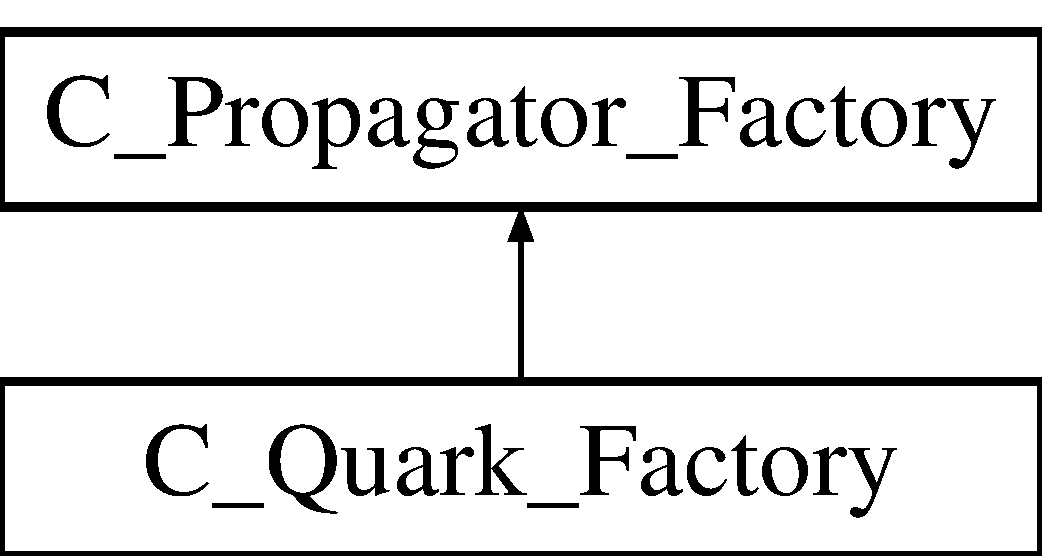
\includegraphics[height=2.000000cm]{class_c___quark___factory}
\end{center}
\end{figure}
\subsection*{Public Member Functions}
\begin{DoxyCompactItemize}
\item 
\hypertarget{class_c___quark___factory_a61cb5db5bb6a0307a36dfd9af4736316}{\hyperlink{class_c___propagator}{C\-\_\-\-Propagator} $\ast$ {\bfseries Create} (int \-\_\-id)}\label{class_c___quark___factory_a61cb5db5bb6a0307a36dfd9af4736316}

\end{DoxyCompactItemize}


The documentation for this class was generated from the following file\-:\begin{DoxyCompactItemize}
\item 
source/\-D\-S\-E/Propagator\-Factory.\-hpp\end{DoxyCompactItemize}

\hypertarget{class_c___quark__parameters}{\section{C\-\_\-\-Quark\-\_\-parameters Class Reference}
\label{class_c___quark__parameters}\index{C\-\_\-\-Quark\-\_\-parameters@{C\-\_\-\-Quark\-\_\-parameters}}
}


{\ttfamily \#include $<$Quark\-\_\-parameters.\-hpp$>$}

\subsection*{Public Member Functions}
\begin{DoxyCompactItemize}
\item 
void \hyperlink{class_c___quark__parameters_a51327f6c5d89e2ab511cf2f7e59428bc}{Print} ()
\item 
void \hyperlink{class_c___quark__parameters_a9281fabcec668955ee7a2edfb1789b6b}{Read\-Parameters} (std\-::string \&\-\_\-\-Param\-Path)
\item 
void \hyperlink{class_c___quark__parameters_aa4d30bbbbfceeff0e5eac01f979139ea}{set\-Default} ()
\end{DoxyCompactItemize}
\subsection*{Public Attributes}
\begin{DoxyCompactItemize}
\item 
int \hyperlink{class_c___quark__parameters_a60916d990db056834babfd4e515b30da}{num\-\_\-prop\-\_\-steps}
\item 
int \hyperlink{class_c___quark__parameters_a28d72426b45b7565713e83ecb42a2d1b}{num\-\_\-cutoff\-\_\-steps}
\item 
int \hyperlink{class_c___quark__parameters_ace76ec22c1f3697f2d17777fa9067657}{num\-\_\-angle\-\_\-steps}
\item 
double \hyperlink{class_c___quark__parameters_aa1f1f3fdad8ccc3c06a012143857599c}{m0}
\item 
double \hyperlink{class_c___quark__parameters_a156667c6701d2542b1a289de58b7b228}{mu}
\item 
double \hyperlink{class_c___quark__parameters_a39f7367e2451ea069cbf763413a800c9}{Lim\-Uk}
\item 
double \hyperlink{class_c___quark__parameters_af40abb13a9312b462c26b4cdd9b21a14}{Lim\-Dk}
\item 
double \hyperlink{class_c___quark__parameters_a86e798ef3a89285c0229612f612eb94f}{M2\-\_\-contour}
\item 
double \hyperlink{class_c___quark__parameters_a1648469ed688b8d25c1ce6a622b90ef7}{Effective\-Cutoff}
\item 
double \hyperlink{class_c___quark__parameters_ab8e384ddf5a6d722a768e7179c4e0c2e}{flag\-\_\-\-Light\-Or\-Heavy\-Quark}
\item 
double \hyperlink{class_c___quark__parameters_ac1e6225033703e6a438930d107df16a3}{Accuracy}
\item 
bool \hyperlink{class_c___quark__parameters_adb9de54db5fdb4d9d326e0d7cfba38a5}{flag\-\_\-load\-Propagator}
\end{DoxyCompactItemize}


\subsection{Detailed Description}
/brief Parameters for a quark

Integration points, bare mass, etc.. 

\subsection{Member Function Documentation}
\hypertarget{class_c___quark__parameters_a51327f6c5d89e2ab511cf2f7e59428bc}{\index{C\-\_\-\-Quark\-\_\-parameters@{C\-\_\-\-Quark\-\_\-parameters}!Print@{Print}}
\index{Print@{Print}!C_Quark_parameters@{C\-\_\-\-Quark\-\_\-parameters}}
\subsubsection[{Print}]{\setlength{\rightskip}{0pt plus 5cm}void C\-\_\-\-Quark\-\_\-parameters\-::\-Print (
\begin{DoxyParamCaption}
{}
\end{DoxyParamCaption}
)}}\label{class_c___quark__parameters_a51327f6c5d89e2ab511cf2f7e59428bc}
\hypertarget{class_c___quark__parameters_a9281fabcec668955ee7a2edfb1789b6b}{\index{C\-\_\-\-Quark\-\_\-parameters@{C\-\_\-\-Quark\-\_\-parameters}!Read\-Parameters@{Read\-Parameters}}
\index{Read\-Parameters@{Read\-Parameters}!C_Quark_parameters@{C\-\_\-\-Quark\-\_\-parameters}}
\subsubsection[{Read\-Parameters}]{\setlength{\rightskip}{0pt plus 5cm}void C\-\_\-\-Quark\-\_\-parameters\-::\-Read\-Parameters (
\begin{DoxyParamCaption}
\item[{std\-::string \&}]{\-\_\-\-Param\-Path}
\end{DoxyParamCaption}
)}}\label{class_c___quark__parameters_a9281fabcec668955ee7a2edfb1789b6b}
\hypertarget{class_c___quark__parameters_aa4d30bbbbfceeff0e5eac01f979139ea}{\index{C\-\_\-\-Quark\-\_\-parameters@{C\-\_\-\-Quark\-\_\-parameters}!set\-Default@{set\-Default}}
\index{set\-Default@{set\-Default}!C_Quark_parameters@{C\-\_\-\-Quark\-\_\-parameters}}
\subsubsection[{set\-Default}]{\setlength{\rightskip}{0pt plus 5cm}void C\-\_\-\-Quark\-\_\-parameters\-::set\-Default (
\begin{DoxyParamCaption}
{}
\end{DoxyParamCaption}
)}}\label{class_c___quark__parameters_aa4d30bbbbfceeff0e5eac01f979139ea}


\subsection{Member Data Documentation}
\hypertarget{class_c___quark__parameters_ac1e6225033703e6a438930d107df16a3}{\index{C\-\_\-\-Quark\-\_\-parameters@{C\-\_\-\-Quark\-\_\-parameters}!Accuracy@{Accuracy}}
\index{Accuracy@{Accuracy}!C_Quark_parameters@{C\-\_\-\-Quark\-\_\-parameters}}
\subsubsection[{Accuracy}]{\setlength{\rightskip}{0pt plus 5cm}double C\-\_\-\-Quark\-\_\-parameters\-::\-Accuracy}}\label{class_c___quark__parameters_ac1e6225033703e6a438930d107df16a3}
\hypertarget{class_c___quark__parameters_a1648469ed688b8d25c1ce6a622b90ef7}{\index{C\-\_\-\-Quark\-\_\-parameters@{C\-\_\-\-Quark\-\_\-parameters}!Effective\-Cutoff@{Effective\-Cutoff}}
\index{Effective\-Cutoff@{Effective\-Cutoff}!C_Quark_parameters@{C\-\_\-\-Quark\-\_\-parameters}}
\subsubsection[{Effective\-Cutoff}]{\setlength{\rightskip}{0pt plus 5cm}double C\-\_\-\-Quark\-\_\-parameters\-::\-Effective\-Cutoff}}\label{class_c___quark__parameters_a1648469ed688b8d25c1ce6a622b90ef7}
\hypertarget{class_c___quark__parameters_ab8e384ddf5a6d722a768e7179c4e0c2e}{\index{C\-\_\-\-Quark\-\_\-parameters@{C\-\_\-\-Quark\-\_\-parameters}!flag\-\_\-\-Light\-Or\-Heavy\-Quark@{flag\-\_\-\-Light\-Or\-Heavy\-Quark}}
\index{flag\-\_\-\-Light\-Or\-Heavy\-Quark@{flag\-\_\-\-Light\-Or\-Heavy\-Quark}!C_Quark_parameters@{C\-\_\-\-Quark\-\_\-parameters}}
\subsubsection[{flag\-\_\-\-Light\-Or\-Heavy\-Quark}]{\setlength{\rightskip}{0pt plus 5cm}double C\-\_\-\-Quark\-\_\-parameters\-::flag\-\_\-\-Light\-Or\-Heavy\-Quark}}\label{class_c___quark__parameters_ab8e384ddf5a6d722a768e7179c4e0c2e}
\hypertarget{class_c___quark__parameters_adb9de54db5fdb4d9d326e0d7cfba38a5}{\index{C\-\_\-\-Quark\-\_\-parameters@{C\-\_\-\-Quark\-\_\-parameters}!flag\-\_\-load\-Propagator@{flag\-\_\-load\-Propagator}}
\index{flag\-\_\-load\-Propagator@{flag\-\_\-load\-Propagator}!C_Quark_parameters@{C\-\_\-\-Quark\-\_\-parameters}}
\subsubsection[{flag\-\_\-load\-Propagator}]{\setlength{\rightskip}{0pt plus 5cm}bool C\-\_\-\-Quark\-\_\-parameters\-::flag\-\_\-load\-Propagator}}\label{class_c___quark__parameters_adb9de54db5fdb4d9d326e0d7cfba38a5}
\hypertarget{class_c___quark__parameters_af40abb13a9312b462c26b4cdd9b21a14}{\index{C\-\_\-\-Quark\-\_\-parameters@{C\-\_\-\-Quark\-\_\-parameters}!Lim\-Dk@{Lim\-Dk}}
\index{Lim\-Dk@{Lim\-Dk}!C_Quark_parameters@{C\-\_\-\-Quark\-\_\-parameters}}
\subsubsection[{Lim\-Dk}]{\setlength{\rightskip}{0pt plus 5cm}double C\-\_\-\-Quark\-\_\-parameters\-::\-Lim\-Dk}}\label{class_c___quark__parameters_af40abb13a9312b462c26b4cdd9b21a14}
\hypertarget{class_c___quark__parameters_a39f7367e2451ea069cbf763413a800c9}{\index{C\-\_\-\-Quark\-\_\-parameters@{C\-\_\-\-Quark\-\_\-parameters}!Lim\-Uk@{Lim\-Uk}}
\index{Lim\-Uk@{Lim\-Uk}!C_Quark_parameters@{C\-\_\-\-Quark\-\_\-parameters}}
\subsubsection[{Lim\-Uk}]{\setlength{\rightskip}{0pt plus 5cm}double C\-\_\-\-Quark\-\_\-parameters\-::\-Lim\-Uk}}\label{class_c___quark__parameters_a39f7367e2451ea069cbf763413a800c9}
\hypertarget{class_c___quark__parameters_aa1f1f3fdad8ccc3c06a012143857599c}{\index{C\-\_\-\-Quark\-\_\-parameters@{C\-\_\-\-Quark\-\_\-parameters}!m0@{m0}}
\index{m0@{m0}!C_Quark_parameters@{C\-\_\-\-Quark\-\_\-parameters}}
\subsubsection[{m0}]{\setlength{\rightskip}{0pt plus 5cm}double C\-\_\-\-Quark\-\_\-parameters\-::m0}}\label{class_c___quark__parameters_aa1f1f3fdad8ccc3c06a012143857599c}
\hypertarget{class_c___quark__parameters_a86e798ef3a89285c0229612f612eb94f}{\index{C\-\_\-\-Quark\-\_\-parameters@{C\-\_\-\-Quark\-\_\-parameters}!M2\-\_\-contour@{M2\-\_\-contour}}
\index{M2\-\_\-contour@{M2\-\_\-contour}!C_Quark_parameters@{C\-\_\-\-Quark\-\_\-parameters}}
\subsubsection[{M2\-\_\-contour}]{\setlength{\rightskip}{0pt plus 5cm}double C\-\_\-\-Quark\-\_\-parameters\-::\-M2\-\_\-contour}}\label{class_c___quark__parameters_a86e798ef3a89285c0229612f612eb94f}
\hypertarget{class_c___quark__parameters_a156667c6701d2542b1a289de58b7b228}{\index{C\-\_\-\-Quark\-\_\-parameters@{C\-\_\-\-Quark\-\_\-parameters}!mu@{mu}}
\index{mu@{mu}!C_Quark_parameters@{C\-\_\-\-Quark\-\_\-parameters}}
\subsubsection[{mu}]{\setlength{\rightskip}{0pt plus 5cm}double C\-\_\-\-Quark\-\_\-parameters\-::mu}}\label{class_c___quark__parameters_a156667c6701d2542b1a289de58b7b228}
\hypertarget{class_c___quark__parameters_ace76ec22c1f3697f2d17777fa9067657}{\index{C\-\_\-\-Quark\-\_\-parameters@{C\-\_\-\-Quark\-\_\-parameters}!num\-\_\-angle\-\_\-steps@{num\-\_\-angle\-\_\-steps}}
\index{num\-\_\-angle\-\_\-steps@{num\-\_\-angle\-\_\-steps}!C_Quark_parameters@{C\-\_\-\-Quark\-\_\-parameters}}
\subsubsection[{num\-\_\-angle\-\_\-steps}]{\setlength{\rightskip}{0pt plus 5cm}int C\-\_\-\-Quark\-\_\-parameters\-::num\-\_\-angle\-\_\-steps}}\label{class_c___quark__parameters_ace76ec22c1f3697f2d17777fa9067657}
\hypertarget{class_c___quark__parameters_a28d72426b45b7565713e83ecb42a2d1b}{\index{C\-\_\-\-Quark\-\_\-parameters@{C\-\_\-\-Quark\-\_\-parameters}!num\-\_\-cutoff\-\_\-steps@{num\-\_\-cutoff\-\_\-steps}}
\index{num\-\_\-cutoff\-\_\-steps@{num\-\_\-cutoff\-\_\-steps}!C_Quark_parameters@{C\-\_\-\-Quark\-\_\-parameters}}
\subsubsection[{num\-\_\-cutoff\-\_\-steps}]{\setlength{\rightskip}{0pt plus 5cm}int C\-\_\-\-Quark\-\_\-parameters\-::num\-\_\-cutoff\-\_\-steps}}\label{class_c___quark__parameters_a28d72426b45b7565713e83ecb42a2d1b}
\hypertarget{class_c___quark__parameters_a60916d990db056834babfd4e515b30da}{\index{C\-\_\-\-Quark\-\_\-parameters@{C\-\_\-\-Quark\-\_\-parameters}!num\-\_\-prop\-\_\-steps@{num\-\_\-prop\-\_\-steps}}
\index{num\-\_\-prop\-\_\-steps@{num\-\_\-prop\-\_\-steps}!C_Quark_parameters@{C\-\_\-\-Quark\-\_\-parameters}}
\subsubsection[{num\-\_\-prop\-\_\-steps}]{\setlength{\rightskip}{0pt plus 5cm}int C\-\_\-\-Quark\-\_\-parameters\-::num\-\_\-prop\-\_\-steps}}\label{class_c___quark__parameters_a60916d990db056834babfd4e515b30da}


The documentation for this class was generated from the following files\-:\begin{DoxyCompactItemize}
\item 
source/\-D\-S\-E/\hyperlink{_quark__parameters_8hpp}{Quark\-\_\-parameters.\-hpp}\item 
source/\-D\-S\-E/\hyperlink{_quark__parameters_8cpp}{Quark\-\_\-parameters.\-cpp}\end{DoxyCompactItemize}

\hypertarget{class_c___strange___quark}{\section{C\-\_\-\-Strange\-\_\-\-Quark Class Reference}
\label{class_c___strange___quark}\index{C\-\_\-\-Strange\-\_\-\-Quark@{C\-\_\-\-Strange\-\_\-\-Quark}}
}


{\ttfamily \#include $<$Quark\-Types.\-hpp$>$}

Inheritance diagram for C\-\_\-\-Strange\-\_\-\-Quark\-:\begin{figure}[H]
\begin{center}
\leavevmode
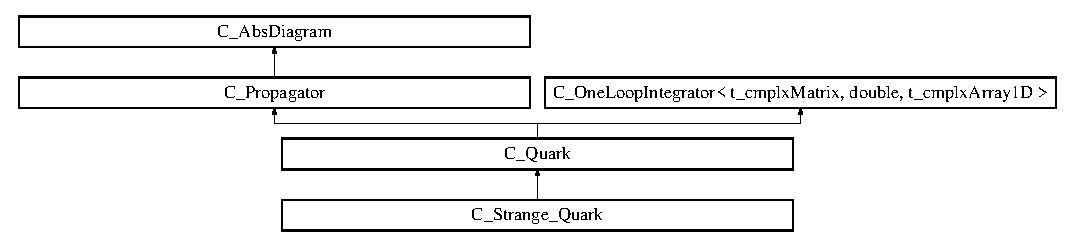
\includegraphics[height=2.871795cm]{class_c___strange___quark}
\end{center}
\end{figure}
\subsection*{Public Member Functions}
\begin{DoxyCompactItemize}
\item 
void \hyperlink{class_c___strange___quark_a0248a7e570a7825efbe2b9064ac2043d}{info} ()
\end{DoxyCompactItemize}
\subsection*{Additional Inherited Members}


\subsection{Member Function Documentation}
\hypertarget{class_c___strange___quark_a0248a7e570a7825efbe2b9064ac2043d}{\index{C\-\_\-\-Strange\-\_\-\-Quark@{C\-\_\-\-Strange\-\_\-\-Quark}!info@{info}}
\index{info@{info}!C_Strange_Quark@{C\-\_\-\-Strange\-\_\-\-Quark}}
\subsubsection[{info}]{\setlength{\rightskip}{0pt plus 5cm}void C\-\_\-\-Strange\-\_\-\-Quark\-::info (
\begin{DoxyParamCaption}
{}
\end{DoxyParamCaption}
)\hspace{0.3cm}{\ttfamily [inline]}}}\label{class_c___strange___quark_a0248a7e570a7825efbe2b9064ac2043d}


The documentation for this class was generated from the following file\-:\begin{DoxyCompactItemize}
\item 
source/\-D\-S\-E/\hyperlink{_quark_types_8hpp}{Quark\-Types.\-hpp}\end{DoxyCompactItemize}

\hypertarget{class_c___test___quark}{\section{C\-\_\-\-Test\-\_\-\-Quark Class Reference}
\label{class_c___test___quark}\index{C\-\_\-\-Test\-\_\-\-Quark@{C\-\_\-\-Test\-\_\-\-Quark}}
}


Specific type for unit testing -\/ all quark parameters are default.  




{\ttfamily \#include $<$Quark\-Types.\-hpp$>$}

Inheritance diagram for C\-\_\-\-Test\-\_\-\-Quark\-:\begin{figure}[H]
\begin{center}
\leavevmode
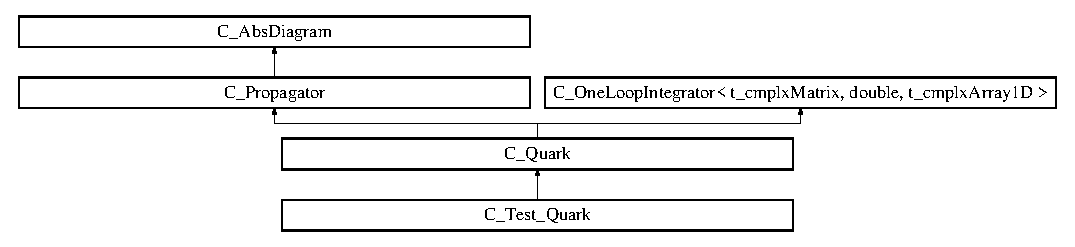
\includegraphics[height=2.871795cm]{class_c___test___quark}
\end{center}
\end{figure}
\subsection*{Public Member Functions}
\begin{DoxyCompactItemize}
\item 
\hypertarget{class_c___test___quark_a34587b5c4031fe77c1b6c6c5c1c76a6a}{void {\bfseries info} ()}\label{class_c___test___quark_a34587b5c4031fe77c1b6c6c5c1c76a6a}

\end{DoxyCompactItemize}
\subsection*{Additional Inherited Members}


\subsection{Detailed Description}
Specific type for unit testing -\/ all quark parameters are default. 

The documentation for this class was generated from the following file\-:\begin{DoxyCompactItemize}
\item 
source/\-D\-S\-E/Quark\-Types.\-hpp\end{DoxyCompactItemize}

\hypertarget{class_c___up___quark}{\section{C\-\_\-\-Up\-\_\-\-Quark Class Reference}
\label{class_c___up___quark}\index{C\-\_\-\-Up\-\_\-\-Quark@{C\-\_\-\-Up\-\_\-\-Quark}}
}
Inheritance diagram for C\-\_\-\-Up\-\_\-\-Quark\-:\begin{figure}[H]
\begin{center}
\leavevmode
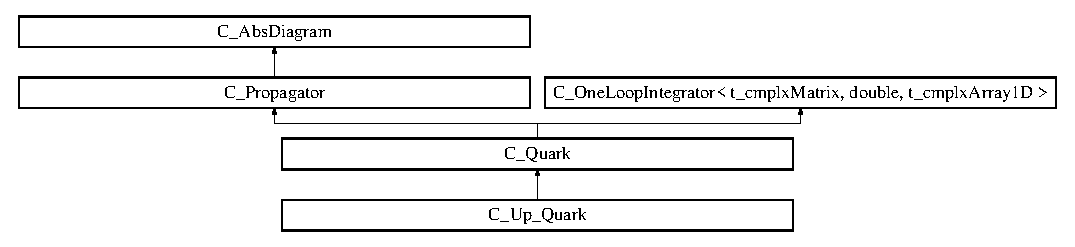
\includegraphics[height=2.871795cm]{class_c___up___quark}
\end{center}
\end{figure}
\subsection*{Public Member Functions}
\begin{DoxyCompactItemize}
\item 
\hypertarget{class_c___up___quark_a37b6df91793cb955f4d66819346121a6}{void {\bfseries info} ()}\label{class_c___up___quark_a37b6df91793cb955f4d66819346121a6}

\end{DoxyCompactItemize}
\subsection*{Additional Inherited Members}


The documentation for this class was generated from the following file\-:\begin{DoxyCompactItemize}
\item 
source/\-D\-S\-E/Quark\-Types.\-hpp\end{DoxyCompactItemize}

\hypertarget{class_interpolation_1_1_linear}{\section{Interpolation\-:\-:Linear$<$ x\-\_\-type, y\-\_\-type $>$ Class Template Reference}
\label{class_interpolation_1_1_linear}\index{Interpolation\-::\-Linear$<$ x\-\_\-type, y\-\_\-type $>$@{Interpolation\-::\-Linear$<$ x\-\_\-type, y\-\_\-type $>$}}
}


Linearly interpolates a given set of points.  




{\ttfamily \#include $<$Linear\-\_\-interpolation.\-hpp$>$}

\subsection*{Public Member Functions}
\begin{DoxyCompactItemize}
\item 
\hyperlink{class_interpolation_1_1_linear_a931383bc431497777e5e0f8c3b43dff3}{Linear} (int n, std\-::vector$<$ x\-\_\-type $>$ \&x, std\-::vector$<$ y\-\_\-type $>$ \&y)
\item 
double \hyperlink{class_interpolation_1_1_linear_a741729571890e0121a85834ca93bf52a}{Real} (\hyperlink{types_8h_aa75ae339052372f671bb263e6a272e82}{t\-\_\-cmplx} x)
\item 
double \hyperlink{class_interpolation_1_1_linear_a5ebf069101fb53752f9591c6b82c3a15}{Real} (double x)
\item 
y\-\_\-type \hyperlink{class_interpolation_1_1_linear_a0293e0e3e3ccff56c979ce054ea6c023}{get\-Value} (x\-\_\-type x)
\end{DoxyCompactItemize}


\subsection{Detailed Description}
\subsubsection*{template$<$typename x\-\_\-type, typename y\-\_\-type$>$class Interpolation\-::\-Linear$<$ x\-\_\-type, y\-\_\-type $>$}

Linearly interpolates a given set of points. 

\subsection{Constructor \& Destructor Documentation}
\hypertarget{class_interpolation_1_1_linear_a931383bc431497777e5e0f8c3b43dff3}{\index{Interpolation\-::\-Linear@{Interpolation\-::\-Linear}!Linear@{Linear}}
\index{Linear@{Linear}!Interpolation::Linear@{Interpolation\-::\-Linear}}
\subsubsection[{Linear}]{\setlength{\rightskip}{0pt plus 5cm}template$<$typename x\-\_\-type, typename y\-\_\-type$>$ {\bf Interpolation\-::\-Linear}$<$ x\-\_\-type, y\-\_\-type $>$\-::{\bf Linear} (
\begin{DoxyParamCaption}
\item[{int}]{n, }
\item[{std\-::vector$<$ x\-\_\-type $>$ \&}]{x, }
\item[{std\-::vector$<$ y\-\_\-type $>$ \&}]{y}
\end{DoxyParamCaption}
)\hspace{0.3cm}{\ttfamily [inline]}}}\label{class_interpolation_1_1_linear_a931383bc431497777e5e0f8c3b43dff3}


\subsection{Member Function Documentation}
\hypertarget{class_interpolation_1_1_linear_a0293e0e3e3ccff56c979ce054ea6c023}{\index{Interpolation\-::\-Linear@{Interpolation\-::\-Linear}!get\-Value@{get\-Value}}
\index{get\-Value@{get\-Value}!Interpolation::Linear@{Interpolation\-::\-Linear}}
\subsubsection[{get\-Value}]{\setlength{\rightskip}{0pt plus 5cm}template$<$typename x\-\_\-type, typename y\-\_\-type$>$ y\-\_\-type {\bf Interpolation\-::\-Linear}$<$ x\-\_\-type, y\-\_\-type $>$\-::get\-Value (
\begin{DoxyParamCaption}
\item[{x\-\_\-type}]{x}
\end{DoxyParamCaption}
)\hspace{0.3cm}{\ttfamily [inline]}}}\label{class_interpolation_1_1_linear_a0293e0e3e3ccff56c979ce054ea6c023}
\hypertarget{class_interpolation_1_1_linear_a741729571890e0121a85834ca93bf52a}{\index{Interpolation\-::\-Linear@{Interpolation\-::\-Linear}!Real@{Real}}
\index{Real@{Real}!Interpolation::Linear@{Interpolation\-::\-Linear}}
\subsubsection[{Real}]{\setlength{\rightskip}{0pt plus 5cm}template$<$typename x\-\_\-type, typename y\-\_\-type$>$ double {\bf Interpolation\-::\-Linear}$<$ x\-\_\-type, y\-\_\-type $>$\-::Real (
\begin{DoxyParamCaption}
\item[{{\bf t\-\_\-cmplx}}]{x}
\end{DoxyParamCaption}
)\hspace{0.3cm}{\ttfamily [inline]}}}\label{class_interpolation_1_1_linear_a741729571890e0121a85834ca93bf52a}
\hypertarget{class_interpolation_1_1_linear_a5ebf069101fb53752f9591c6b82c3a15}{\index{Interpolation\-::\-Linear@{Interpolation\-::\-Linear}!Real@{Real}}
\index{Real@{Real}!Interpolation::Linear@{Interpolation\-::\-Linear}}
\subsubsection[{Real}]{\setlength{\rightskip}{0pt plus 5cm}template$<$typename x\-\_\-type, typename y\-\_\-type$>$ double {\bf Interpolation\-::\-Linear}$<$ x\-\_\-type, y\-\_\-type $>$\-::Real (
\begin{DoxyParamCaption}
\item[{double}]{x}
\end{DoxyParamCaption}
)\hspace{0.3cm}{\ttfamily [inline]}}}\label{class_interpolation_1_1_linear_a5ebf069101fb53752f9591c6b82c3a15}


The documentation for this class was generated from the following file\-:\begin{DoxyCompactItemize}
\item 
source/\-Num\-Libs/\hyperlink{_linear__interpolation_8hpp}{Linear\-\_\-interpolation.\-hpp}\end{DoxyCompactItemize}

%--- End generated contents ---

% Index
\newpage
\phantomsection
\addcontentsline{toc}{chapter}{Index}
\printindex

\end{document}
